%\documentclass[a4paper,12pt]{eskdtext} %размер бумаги устанавливаем А4, шрифт 12пунктов
\documentclass[a4paper,14pt]{scrartcl} %размер бумаги устанавливаем А4, шрифт 12пунктов
%\documentclass[14pt,a4paper,twoside]{report}
\usepackage[T2A]{fontenc}
\usepackage[utf8]{inputenc} %включаем свою кодировку: koi8-r или utf8 в UNIX, cp1251 в Windows
\usepackage[english,russian]{babel} %используем русский и английский языки с переносами
\usepackage{amssymb,amsfonts,amsmath,mathtext,cite,enumerate,float} %подключаем нужные пакеты расширений
\usepackage[dvips]{graphicx} %хотим вставлять в диплом рисунки?
%\usepackage{soul}
\usepackage[14pt]{extsizes}
\usepackage{longtable}
\usepackage{graphicx}
\usepackage{indentfirst}
\usepackage{enumerate}
\usepackage{xcolor}

\graphicspath{{../images/}} %путь к рисункам

%\linespread{1.5}

\usepackage[format=plain,labelformat=simple,labelsep=endash,figurename=\CYRR\cyri\cyrs\cyru\cyrn\cyro\cyrk]{caption}
\captionsetup{figurewithin=section} % картинки нумеруются относительно секций
\numberwithin{equation}{section} % нумерация формул внутри раздела
\numberwithin{table}{section}

\makeatletter
\renewcommand{\@biblabel}[1]{#1.} % Заменяем библиографию с квадратных скобок на точку:
\makeatother

\RequirePackage{lscape}

%\renewcommand\large{\@setfontsize\large{15.5}{17}}
%\renewcommand\Large{\@setfontsize\Large{16.5}{19}}
%\renewcommand\small{\@setfontsize\small{9}{9.5}}

\usepackage{geometry} % Меняем поля страницы
\geometry{left=2cm} % левое поле
\geometry{right=1cm} % правое поле
\geometry{top=2cm} % верхнее поле
\geometry{bottom=2cm} % нижнее поле

\renewcommand{\theenumi}{\arabic{enumi}} % Меняем везде перечисления на цифра.цифра
\renewcommand{\labelenumi}{\arabic{enumi}} % Меняем везде перечисления на цифра.цифра
\renewcommand{\theenumii}{\arabic{enumii}} % Меняем везде перечисления на цифра.цифра
\renewcommand{\labelenumii}{\arabic{enumi}.\arabic{enumii}.}% Меняем везде перечисления на цифра.цифра
\renewcommand{\theenumiii}{\arabic{enumiii}} % Меняем везде перечисления на цифра.цифра
\renewcommand{\labelenumiii}{\arabic{enumi}.\arabic{enumii}.\arabic{enumiii}.}% Меняем везде перечисления на цифра.цифра

\renewcommand{\baselinestretch}{1.5}

% redefine title and bibl
\addto\captionsrussian{\def\contentsname{Содержание}}
%\addto\captionsrussian{\def\bibname{Список литературы}}
\addto\captionsrussian{\def\refname{Список используемых источников}}
 % main tamplate

\begin{document}
%\input{title} % это титульный лист
%\input{diplom_task}
\tableofcontents % это оглавление, которое генерируется автоматически
\newpage

%\addcontentsline{toc}{section}{ВВЕДЕНИЕ}
\section*{ВВЕДЕНИЕ}

Большое количество современных систем являются беспроводными. Простота развертывания, мобильность, относительно низкая
стоимость - вот основные преимущества беспроводных систем. Количество мобильных устройств (телефоны, планшетные компьютеры
и т.д.) с каждым годом стремительно растет, только мобильных телефонов в 2011 году было 5.6 миллиарда и покрывало 79.86\%
\cite{wiki_mobilenum} населения земли. Технологии беспроводной связи глубоко проникли во все сферы жизни общества:
обеспечение безопасности с помощью RFID датчиков, предоставление доступа в интернет по технологиями 3G, WiFi, 
сотовая связь по различным технологиям (GSM, CDMA, DAMPS). Некоторые из этих систем строятся на основе методики
расширения спектра, которая отвечает современным требованиям по мощности сигнала, а так же по безопасности передаваемых
данных. В основе таких систем лежат шумоподобные (широкополосные) сигналы - ШПС. Вместе с тем растут требования к таким
системам. Применение ШПС ставит ряд специфических задач по обработке информации, обусловленных особенностями ШПС.
Свойства характерные для ШПС, выгодно отличают данный класс систем от класса узкополосных систем, но с другой стороны
оборачивается усложнением методов обработки ШПС.

Внедрение новых технологий требует увеличение полосы частот. Разнообразие технологий беспроводной передачи данных среди
гражданских и военных систем ведет к перегрузке каналов связи и все более высоким требованиям к скорости передачи
данных. С учётом данных требований применение систем передачи информации с ШПС становится все более востребованным.

Принимая во внимание географические размеры России и стратегическую важность обладания собственными системами спутникового
позиционирования, правительство Российский Федерации уделяет особое внимание разработке собственной системы
глобального спутникового позиционирования ГЛОНАСС. Обладание собственными технологиями системы спутниковой навигации (СНС), государство может обезопасить
себя в случае военных конфликтов от ограничения применения американской системы СНС Navstar GPS в зоне конфликта.

Разработка систем, позволяющих работать с несколькими различными СНС, позволит повысить точность определения координат
в сложных условиях города. Сложность детектирования сигнала и определения координат обусловлена наличием плотной
застройки многоэтажными зданиями. В городских условиях задача подавления интерференционной помехи становится особенно
актуальной. Спектр интерференционной помехи не является белым, а фильтрация и компенсация цветного шума
требует разработки специальных алгоритмов.

Новые цифровые процессоры позволяют применять подходы, которые еще 10-15 лет назад были бесперспективными.
В данной работе развиваются подходы на основе построения параметрической модели ШПС. Невозможность использования
методов требующих вычислений с высокой точностью в приемниках реального времени
10-15 лет назад была обусловлена слабой производительностью процессоров и микроконтроллеров, а так же существенной
стоимостью процессоров с модулем для операций с числами с плавающей точкой. Современное развитие цифровых технологий делает 
возможным применение параметрических методов оценки спектра взамен традиционного подхода основанного на непараметрического
анализа спектра.

Основа теории систем связи с ШПС была заложена в работах В.А. Котельникова и К. Шеннона.
России в этой области занимались В.И. Борисов, В.Б. Пестряков, В.И. Журавлев, М.И. Жодзишский, Б.И. Шахтарин, Л.Е.  Варакин, В.Е. Гантмахер и др.

Изначально методы расширенного спектра применялись при разработке военных систем управления и связи \cite{sklyar}.
К концу второй мировой войны расширение спектра применялось в радиолокации для борьбы с преднамеренными помехами, а
в последствии развитие данной технологии объяснялось желанием создать помехоустойчивые системы связи.
В конце 40-х-начале 50-х годов прошлого века Мортимер Рогофф, сотрудник Международной Телефонной и Телеграфной Корпорации (США) (ITT),
провёл эксперимент по передаче информации при помощи псевдошумового сигнала \cite{sklyar}, среди отечественных ученых
в середине 30-х годов прошлого века работу об основах кодового разделения каналов написал Д.В. Агеев.
Первые разработки таких систем относились к военным отраслям. Данный факт объясняется рядом особенностей, которыми обладают
сигналы с расширенным спектром, в числе которых — сложность перехвата заложенной в них информации,
высокая помехоустойчивость, а также трудность обнаружения факта работы передатчика. В процессе исследований расширенному спектру
нашлось и другое применение - снижение плотности энергии, высокоточная локация, использование при множественном доступе
\cite{sklyar}

Системы связи с широкополосными сигналами занимают особое место. Их особенные свойства выделяют данный класс из других систем
связи. Высокая помехозащищенность при действии сильной помехи, кодовое разделение большого количества абонентов, прием
информации с высокой достоверностью - отличительные особенности широкополосных система. Эти черты были известно, но
уровень элементной базы и низкий уровень помех не позволяли получить развития системам данного класса. Однако развитие
элементной привело к широкому распространению данного вида сигналов. В настоящее они применяются в системах спутниковой навигации,
системах сотовой связи и др \cite{varakin-book}.

Отношение сигнал/шум (ОСШ) на входе приемника может быть очень низким. Для обеспечения высокой помехозащищенности 
в таких случаях используются ШПС с большими и сверхбольшими базами.

К созданию сложных широкополосных сигналов (СШС) привело решение ряда проблем при развитии систем передачи данных.
Первая проблема встала при разработке новых радиолокационных система. Для дальнейшего развития требовалось
решить несколько противоречий: требование высокой разрешающей способности по дальности и дальностью обнаружения
целей в импульсных РЛС, требование точного измерения скорости и высокое разрешение по дальности, требование
увеличить дальность при ограничении пиковой мощности \cite{gantmaher-book}. Решение данных задач было предложено
Ф. Вудвардом. Им было показано, что дополнительным параметром является форма сигнала. Длительность сигнала
может быть больше - настолько больше, насколько это необходимо для обеспечения энергетических требований, а требование
разрешения по дальности и точности измерений определяются шириной полосы сигнала. Данные требования обеспечивается
путем сжатия импульса на стороне приемника. Вудворд сформулировал принципы: произведение эффективной полосы частот
радиосигнала на его длительность должен быть существенно больше единиц ${FT>>1}$, внутренняя структура сигнала
должна быть такой, чтобы обеспечить возможность приемнику сжатие распределенного во времени сигнала в короткий импульс,
соответствующий полосе ${F}$ \cite{gantmaher-book}.

В \cite{gantmaher-book} показана связь пропускной способности канала с понятием ШПС. При ${R_e<<1}$ можно записать:
\begin{center}
\begin{equation}
	\label{eq:shennon_cdma}
	FT = \frac{1}{\log(1+R_e)},
\end{equation}
\end{center}
где ${R_e}$ - ОСШ, ${F}$ - эффективная полоса частот, ${T}$ - длительность.

Стоить отметить, что при ${R_e<<1}$, левая часть выражения \ref{eq:shennon_cdma} стремится к бесконечности, а значит
ШПС позволяет обеспечить теоретически неограниченную достоверность передачи информации. Второе важное свойство
ШПС, следующее из \ref{eq:shennon_cdma} - способность работать "под шумами". Что обеспечивает скрытность
передачи информации, а с другой высокую степень уплотнения каналов связи и, как следствие, решение современных проблем
с перегруженностью каналов связи.

В данной работе будет рассматриваться ШПС модулированный ПСП на основе двоичной рекуррентной последовательности.
Для выделения данных из потока необходимо иметь точно синхронизированную копию ПСП, которая была использована
при модулировании сигнала на передающей стороне. Для достижения синхронизма на стороне приемника необходимо
устранить неопределенность в двух областях: неопределенность по частоте и неопределенность по фазе (задержке) ПСП.
Неопределенность по фазе ПСП обусловлена неопределенностью в расстоянии между передатчиком и приемником. Неопределенность
по частоте обусловлена в первую очередь допплеровским эффектом, а так же нестабильностью опорных генераторов в
передатчике и приемнике. После устранения неопределенности по частоте для достижения точной синхронизации
начинается процесс слежения за частотой. Неопределенность по фазе ПСП устранить, не используя полный перебор,
невозможно в силу корреляционных свойств ПСП. Таким образом можно заключить, что задача быстрого и эффективного
поиска и оценки параметров ШПС является актуальной.

В данной работе рассматривается подход программного приемника (Software Defined Receiver - SDR)
\cite{akos-book, grayver-book, pany-book} для оценки параметров ШПС. Как уже было отражено выше, ШПС применяется во
многих системах. В данной работе для полунатурного эксперимента будет рассматриваться сигнал СНС Navstar GPS. Данная система передачи 
информации использует ПСП Голда \cite{gold-ieee} для модулирования сигнала.

Традиционные подходы к реализации приемника СНС Navstar GPS отражены в \cite{akos-book, tsui}. 

Популярность и распространенность данной системы стимулирует исследования в области детектирования
и оценки частоты ШПС сигналов.

Существуют исследования в области применения теории хаоса - детектирование и оценка
частоты ШПС с применением осциллятора Дуффинга \cite{chaos_cambridge, chaos_chen, chaos_huang, chaos_wang}. Преимуществом
данного подхода является то, что свойства осциллятора позволяют детектировать сигналы с экстремально низким ОСШ. В то же
время, на данный момент никто не предложил цифровое представление осциллятора Дуффинга, а это затрудняет использование данного подхода
в реальных приемниках. Таким образом данное направление является в настоящее время больше теоретическим, чем практическим.

В работах \cite{hos_petropulu, hos_zhao} предложено использовать статистики высоких порядков для подавления шума и детектирование
сигналов с низким уровнем ОСШ.

Более традиционные подходы для детектирования и оценки параметров ШПС сигналов с низким уровнем ОСШ рассмотрены в монографии \cite{ziedan-book}.
В данной монографии рассматриваются как методы детектирования и оценки параметров ШПС, основанные на когерентном накоплении, так и эффективные
системы слежения за частотой и фазой ПСП.

{\bf{Добавить ЦЕЛИ И ЗАДАЧИ}}

%%%%%%
\paragraph{Постановка задачи оценки параметров сигнала с расширенным спектром.}
В данной работе рассматриваются задачи повышения рабочих характеристик приемников ШПС, поэтому целесообразно отразить основные модули этой системы 
на примере СНС Navstar GPS - рисунок \ref{pic:sec1_gnss_system}.
\begin{figure}[H]
\center\scalebox{1}{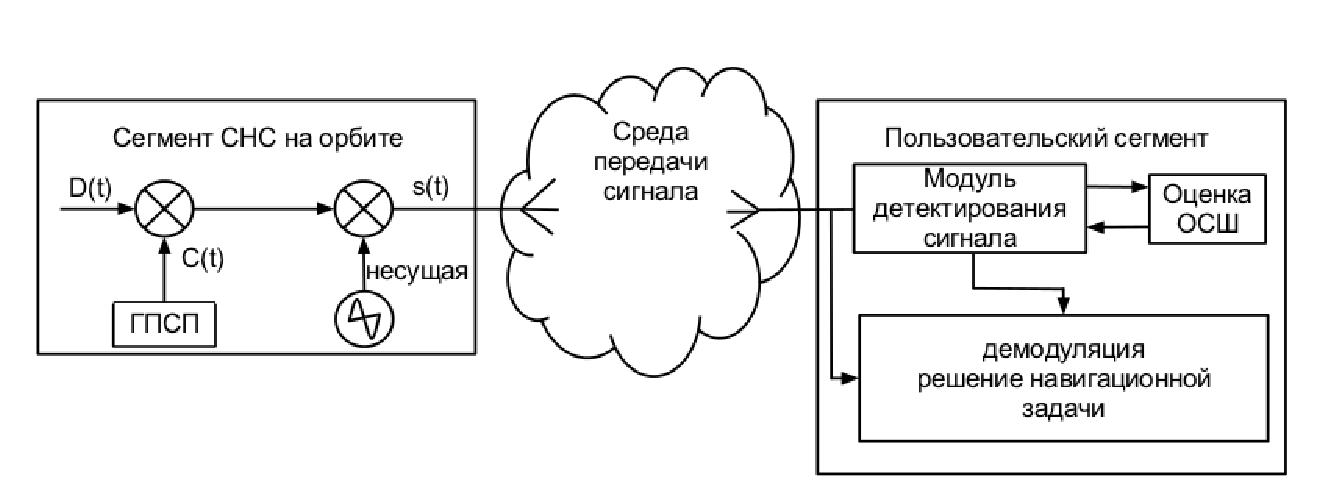
\includegraphics[width=1\linewidth]{sec1gnss_system.eps}}
\caption{структутраная схема СНС GPS}
\label{pic:sec1_gnss_system}
\end{figure}

В систему СНС Navstar GPS входят космический сегмент, наземный сегмент (на рисунке \ref{pic:sec1_gnss_system} не
отражен), а так же пользовательский сегмент. В космический сегмент входит спутниковая группировка, в 
наземный - станции управления, в пользовательский - все устройства принимающие сигнал от СНС GPS.

\paragraph{Модель сигнала и помех.}
В системе СНС Navstar GPS применяется ШПС.
Система передачи информации считается системой с расширенным спектром в следующих случаях \cite{sklyar}:
\begin{enumerate}
	\item Используемая полоса значительно шире минимальной, необходимой для передачи данных.
	\item Расширение спектра производится с помощью так называемого расширяющего сигнала (ПСП),
		который не зависит от передаваемой информации.
	\item Восстановление исходных данных ("сужение спектра") осуществляется путем сопоставления полученного
		сигнала и синхронизированной копии расширяющего сигнала (ПСП)
\end{enumerate}

Так же подобные сигналы называют:
\textquotedblleftсложными\textquotedblright,
\textquotedblleftшумоподобными\textquotedblright,
\textquotedblleftпсевдослучайными\textquotedblright,
\textquotedblleftсложными-дискретными\textquotedblright,
\textquotedblleftдискретно-кодированными\textquotedblright,
\textquotedblleftортогональными (квазиортогональными)\textquotedblright,
\textquotedblleftоптимальными дискретными\textquotedblright
\cite{gantmaher-book}.

Каждое название ставит акцент на определенной характеристике сигнала. В данной работе я буду оперировать термином
широкополосный сигнал - ШПС. ШПС можно определить как \cite{gantmaher-book, varakin-book}:
\begin{center}
\begin{equation}
	\label{eq:ss_signal}
	1 << FT = B,
\end{equation}
\end{center}
где: ${B}$ - база сигнала, ${F}$ - эффективная ширина спектра, а ${T}$ - длительность.
Неточность этого определения рассмотрена в \cite{gantmaher-book}, так же там даны ссылки на другие источники
разделяющие критику данного определения. Для данной работы критика, рассмотренная в приведенных источниках,
принципиального значения не имеет.

%%%%%%
\paragraph{Классическая постановка задачи оценки параметра.}
Из литературы по теории автоматических систем, например \cite{pugachev} (глава 10.1), известна классическая постановка
задачи задачи теории оптимальных систем. "На практике часто приходится решать задачу проектирования системы, когда
требуется определить характеристики системы таким образом, чтобы она имела наибольшую точность при данных условиях.
Систему обеспечивающую наибольшую возможную точность с какой-нибудь определенной точки зрения среди всех систем
заданного класса, обычно называют оптимальной" \cite{pugachev}.

В одной из постановок данной задачи \cite{pugachev} (глава 10.1), система считается полностью неизвестной
и требуется определить ее оператор так, чтобы она была оптимальной с точки зрения принятого критерия качества. Эта
задача сводится к определению с наибольшей возможной точностью некоторых параметров, от которых зависит принимаемый
сигнал. Но при этом важно учитывать не только точность, но и другие факторы, так как проектируемая система должна
удовлетворять многим, часто противоречивым требованиям. В виду приведенных факторов, обычно представляет собой
ряд компромиссных решений, удовлетворяющих всем предъявляемым к системе требованиям.

Точность автоматической системы обычно характеризуется математическим ожиданием и дисперсией ее ошибки.
Математическое ожидание представляет собой систематическую ошибку системы в данных условиях, а дисперсия
характеризует уровень случайных ошибок \cite{pugachev} (глава 10.2). Так как в различных условиях работы
системы, которые встречаются случайно систематическая ошибка тоже является случайной, за критерий качества
системы при ее проектировании обычно принимают второй начальный момент ошибки - математическое ожидание
квадрата ошибки:
\begin{center}
\begin{equation}
	\label{eq:stat_err_prob}
	\eta = M[e^2(t)]
\end{equation}
\end{center}
Положительный квадратный корень из этой величины называют средней квадратичной ошибкой системы. Таким образом,
оптимальной системой обычно считают такую систему, которая имеет минимальную среднюю квадратичную ошибку.

Критерий минимума средней квадратичной ошибки является простейшим с математической точки зрения и обычно приводит
к наиболее простым методам определения оптимальных систем. Однако далеко не во всех задачах он может служить мерой
качества системы. Поэтому нельзя ограничиваться методами нахождения оптимальных систем по критерию минимума средней
квадратичной ошибки.

В случаях, когда необходимо проектировать следящую систему, приходится учитывать возможность срыва слежения,
который заключается в том что система перестает работать, если ее ошибка превосходит по абсолютной величине некоторый
уровень. При проектировании таких систем целесообразно принять за критерий качества вероятность срыва слежения. При
этом оптимальной считается такая система, которая обеспечивает минимум вероятности срыва слежения. Если срыв слежения
происходит в случае, когда абсолютная величина ошибки превосходит уровень $a$, то критерий минимума вероятности ошибки
слежения можно представить \cite{pugachev} (глава 10.2):
\begin{center}
\begin{equation}
	\label{eq:prob_lost_signal}
	p = P(e(t) > a) = min
\end{equation}
\end{center}

%%%%%%
\paragraph{Введение обозначений.}
В диссертации рассматривается сигнал с расширенным спектром полученный методом "прямой последовательности".
Данный метод заключается в том, что гармоническая несущая сигнала модулируется высокоскоростным (широкополосным)
расширяющим сигналом (ПСП). 

Несущее колебание с частотой ${\omega_0}$  модулируется данными ${d(t)}$ , а также высокоскоростной ПСП ${g(t)}$, полученной методом "прямой последовательности".
СПИ Navstar GPS осуществляется двоичная фазовая модуляция (ДФМ или 2-ФМ), а значит ${d(t)}$  и ${g(t)}$  - потоки антиподных импульсов \{-1, 1\}.
Таким образом сигнал на выходе модулятора может быть представлен \cite{shahtarin_sync}:
\begin{equation}
	\label{eq:cdma_eq}
	s(t)=Ad(t)g(t)\cos{(\omega_{0}t)},
\end{equation}
где ${d(t)}$- информационный бит, а ${g(t)}$ - ПСП представляет собой фазовый сдвиг  ${0, \pi}$.

В реальных СПИ сигнал на приемник поступает одновременно от нескольких источников, присутствует неопределенность по частоте, а также аддитивный белый шум (АБГШ).
В приемнике после оцифровки сигнала получаем смесь:
\begin{equation}
	\label{eq:cdma_strip_eq}
	x(m)=\sum_{k=1}^{N}\left( A_k g(m + \tau_k)\exp{\left[j \left( \tilde{\omega}_{k}m + \phi_k(m)\right)\right]} \right) + n(m),
\end{equation}
где  ${k}$ - относительный номер источника сигнала, ${N}$ - количество доступных источников сигнала, модулированных ПСП одного семейства,
${m}$ - индекс соответствующий времени, ${\tilde{\omega}_{k}}$  – относительная частота, соответствующая ${\omega_0}$,
${\tau_k}$ - задержка модулирующей ПСП в точке приема, ${\phi_k(m)}$ - случайная начальная фаза, ${n(m)}$ - аддитивный белый гауссов шум (АБГШ). 

Следует отметить, что при оценке фазы сигнала с номером ${k}$  интерференцией являются сигналы:    .
\begin{equation}
	%\label{eq:cdma_interference}
	\{n \ne k, n \in [1,N]\}
\end{equation}

%%%%%%
\paragraph{Алгоритмы оценки параметров широкополосного сигнала сигнала.}
Алгоритм реализующий метод максимального правдоподобия - последовательный коррелятор. Данный подход реализуется в аппаратных приемниках.
Аппаратный приемник позволяет реализовать параллельно несколько последовательных корреляторов и вести оценку параметров
СПИ с ШПС параллельно.

Данный алгоритм в некоторых источниках так же называется согласованным фильтром. В \cite{sklyar} рассмотрены нюансы этих двух понятий.
В данной работе используется понятие последовательный коррелятор. Работа коррелятора описывается математической операцией
корреляции \ref{eq:serial_corr}. Сигнал коррелируется с локальной копией и на выходе коррелятора получается значение, отражающее
степень совпадения сигналов. Не трудно представить, что сигнал с хорошими корреляционными свойствами должен обладать высоким значением
корреляции когда сигналы синхронизированы и минимальным значением в любом другом случае (фаза ПСП не выровнена - отсутствие сигнала).
\begin{equation}
	\label{eq:serial_corr}
	y(n)=\sum\limits_{m=0}^{N-1}{x(m)h(n+m)},
\end{equation}
где ${x(m)}$ - принятая смесь, а ${h(n)}$ не импульсная характеристика системы, а локальная копия сигнала.

%%%%%%%%
% DFT

Вычисление циклической свертки через дискретное преобразование Фурье (ДПФ) - достаточно популярный метод
в программных приемниках, так как позволяет существенно уменьшить количество операций при вычислении. Но, как показано
в \cite{tsui, oppenheim}, можно достаточно просто перейти от свертки к циклической корреляции. Так как этот метод является самым
популярным в программных приемниках стоит его представить.
Свертка может быть представлена как:
\begin{equation}
	\label{eq:fft_conv}
	y(n)=\sum\limits_{m=0}^{N-1}{x(m)h(n-m)}
\end{equation}

Стоит отметить, что в \ref{eq:fft_conv} сдвиг во времени является циклическим, поскольку дискретные операции являются циклическими.
Возьмем ДПФ от \ref{eq:fft_conv}
\begin{center}
\begin{eqnarray}
	\label{eq:fft_conv_fft}
	Y(k) & = & \sum\limits_{n=0}^{N-1}\sum\limits_{m=0}^{N-1}{x(m)h(n-m)e^{(-j2\pi{kn})/N}}=\nonumber \\
	& = & \sum\limits_{m=0}^{N-1}{x(m)}[\sum\limits_{n=0}^{N-1}h(n-m)e^{(-j2\pi{(n-m)}k)/N}]e^{(-j2\pi{m}k)/N}=\\
	& = & H(k)\sum\limits_{m=0}^{N-1}e^{(-j2\pi{m}k)/N} = X(k)H(k)\nonumber 
\end{eqnarray}
\end{center}
Из уравнения \ref{eq:fft_conv_fft} легко видеть, что это не линейная свертка. В линейной свертке для входного сигнала размером в ${N}$ точек,
результат будет из ${2N-1}$ точек. А в уравнении выше, результатом является всего ${N}$ точек.
Это проявление циклической природы ДПФ.

Алгоритм оценки не использует свертку, он использует корреляцию, которая отличается от свертки. Корреляция
между $x(n)$ и $h(n)$ записывается выражением \ref{eq:serial_corr}:
Единственным отличаем между \ref{eq:serial_corr} и \ref{eq:fft_conv} является знак перед $m$ в ${h(n+m)}$.
В случае оценки параметра ШПС, $h(n)$ является локальной копией сигнала, а не импульсной характеристикой.
Произведем ДПФ над $z(n)$:
\begin{center}
\begin{eqnarray}
	\label{eq:fft_corr_fft}
	Z(k) & = & \sum\limits_{n=0}^{N-1}\sum\limits_{m=0}^{N-1}{x(m)h(n+m)e^{(-j2\pi{kn})/N}}=\nonumber \\
	& = & \sum\limits_{m=0}^{N-1}{x(m)}[\sum\limits_{n=0}^{N-1}h(n+m)e^{(-j2\pi{(n+m)}k)/N}]e^{(j2\pi{m}k)/N}=\\
	& = & H(k)\sum\limits_{m=0}^{N-1}e^{(j2\pi{m}k)/N} = X(k)H^{-1}(k)\nonumber 
\end{eqnarray}
\end{center}
где ${X^{-1}(k)}$ - обратное ДПФ. Уравнение \ref{eq:fft_corr_fft} можно записать как:

\begin{equation}
	\label{eq:fft_corr_fft_rev}
	Y(k) = \sum\limits_{n=0}^{N-1}\sum\limits_{m=0}^{N-1}{x(n+m)h(m)e^{(-j2\pi{kn})/N}}=X^{-1}(k)H(k)
\end{equation}

Если сигнал $x(n)$ действительный, то $x(n) = x^*(n)$, где ${^*}$ - операция комплексного сопряжения. Используя данное соотношение,
значение $Z(k)$ может быть записано:
\begin{equation}
	\label{eq:fft_magnitude}
	|Z(k)|=|H^*(k)X(k)|=|H(k)X(k)^*|
\end{equation}
Данное соотношение может быть использовано для нахождения значения циклической корреляции между входным сигналом и 
локальной копией.

%%%%%%%%
% Chaos 
Оценка параметров СПИ с ШПС (в частности сигналов системы Navstar GPS) с помощью осциллятора Дуффинга
достаточно новое направление в исследованиях по данной тематике. В данной области опубликовано несколько работ, в частности \cite{chaos_chen, chaos_cambridge, chaos_huang, chaos_song}.
Так же является интересной более ранняя статья не рассматривающая GPS \cite{chaos_wang}.
Осциллятор Дуффинга с гармоническим внешним воздействием может быть описан уравнением:
\begin{center}
\begin{equation}
	\label{eq:duffing}
	mx'' + cx' + k_{1}x + k_{2}x^3 = F_{0}\cos(\omega{t}),
\end{equation}
\end{center}
где $m$ - масса, $c$ - коэффициент диссипации, $x$ - состояние осциллятора, $k_1$ и $k_2$ - линейный и нелинейный коэффициенты соответственно,
$F_{0}\cos(\omega{t})$ - внешнее воздействие.

Подробно уравнение \ref{eq:duffing} рассмотрено в \cite{chaos_neimark_landa}.
Для использования осциллятора Дуффинга с целью оценки параметров ШПС была предложена усовершенствованная форма \cite{chaos_song, chaos_chen}:
\begin{center}
\begin{equation}
	\label{eq:duffing_gps}
	x'' +cx' - x^3 + x^5 = \gamma\cos(\omega{t}) + (\gamma_{x}\cos(\omega_{x}) + n(t))
\end{equation}
\end{center}

Перепишем динамическую систему \ref{eq:duffing_gps} в виде:
\begin{center}
\begin{equation}
	\label{eq:duffing_gps_2}
	\left\{
	\begin{aligned}
		y(t) & = x'(t) \\
		y'(t) & =  -cx' + x^3 - x^5 + \gamma\cos(\omega{t}) + (\gamma_{x}\cos(\omega_{x}) + n(t)),
	\end{aligned}
	\right.
\end{equation}
\end{center}
где ${n(t)}$ - АБГШ.

Пример фазового портрета при ${\omega=\omega_{x}}$ изображен на рисунке \ref{pic:duffing_sync},
фазовый портрет хаоса расположен на рисунках \ref{pic:duffing_chaos1}, \ref{pic:duffing_chaos2}
\begin{figure}[H]
	\center\scalebox{0.5}{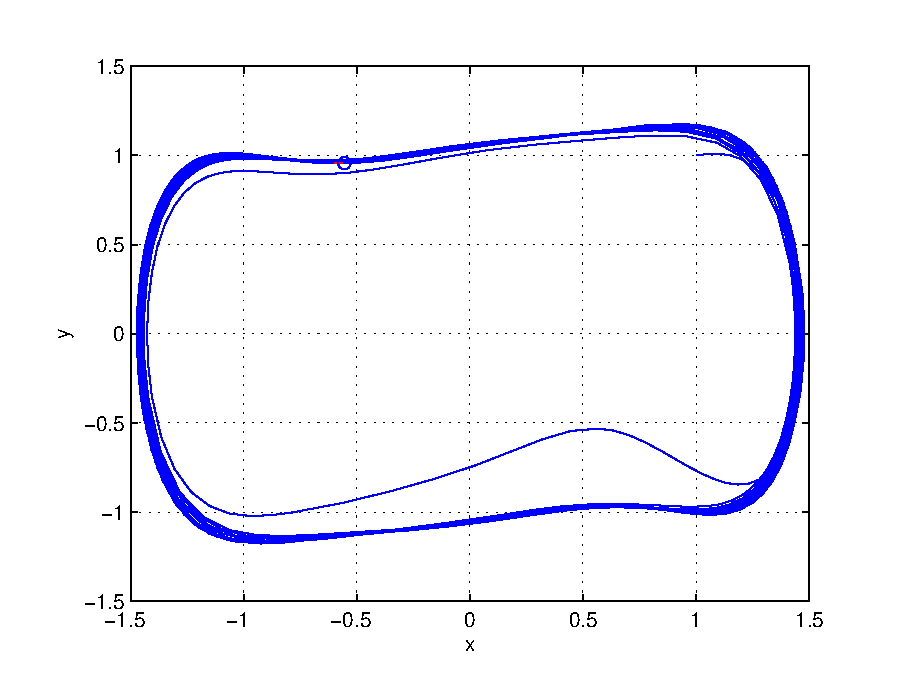
\includegraphics[width=1\linewidth]{duffing_sync.eps}}
	\caption{Фазовый портрет при ${\omega =\omega_{x}}$}
	\label{pic:duffing_sync}
\end{figure}
\begin{figure}[H]
	\center\scalebox{0.5}{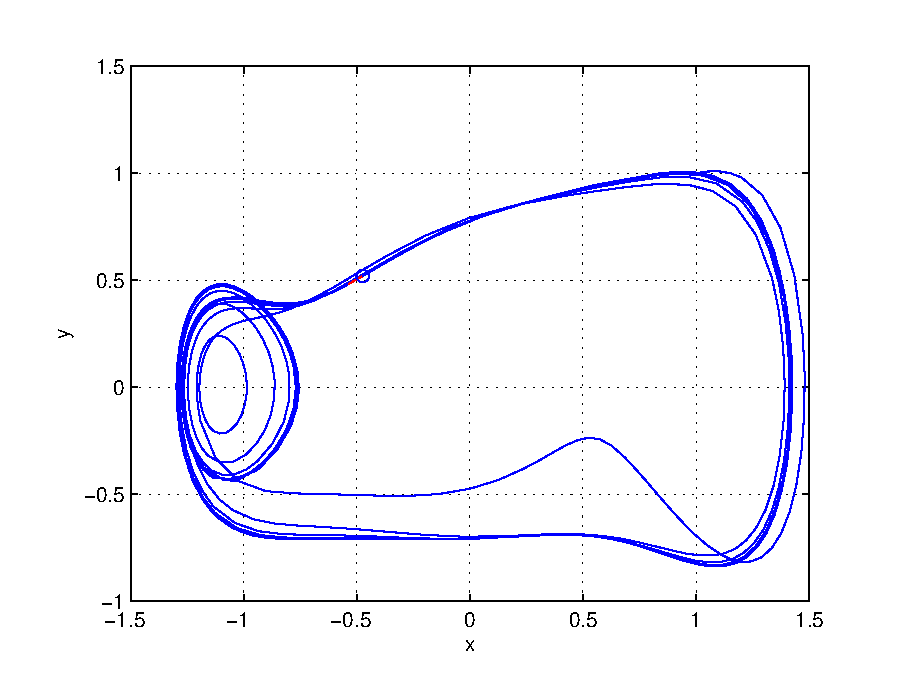
\includegraphics[width=1\linewidth]{duffing_chaos1.eps}}
	\caption{Фазовый портрет при ${\omega < \omega_{x}}$}
	\label{pic:duffing_chaos1}
\end{figure}
\begin{figure}[H]
	\center\scalebox{0.5}{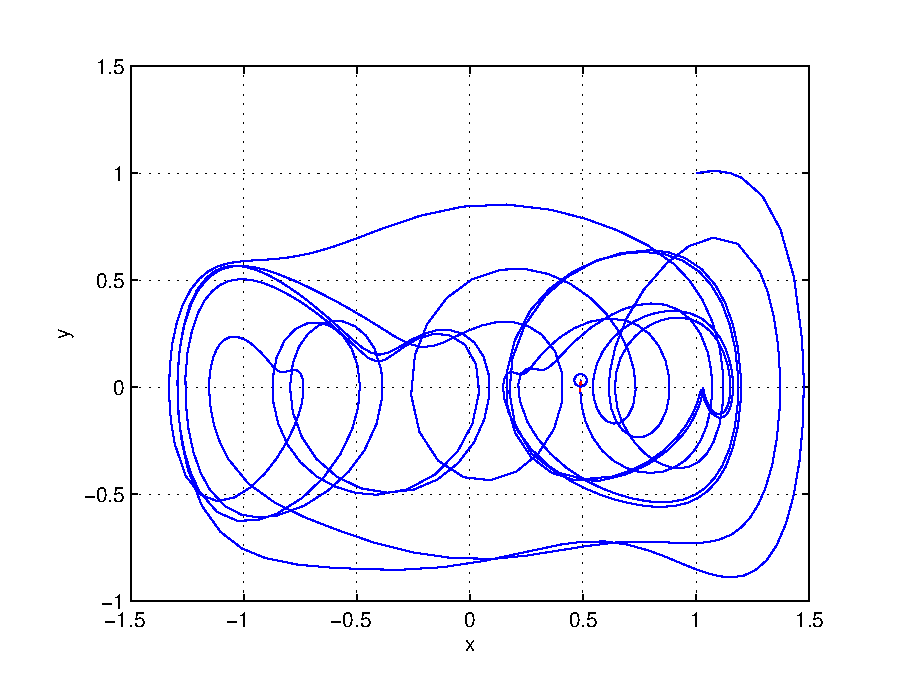
\includegraphics[width=1\linewidth]{duffing_chaos2.eps}}
	\caption{Фазовый портрет при ${\omega > \omega_{x}}$}
	\label{pic:duffing_chaos2}
\end{figure}
В качестве параметров уравнения применялись: $c = 0.5$, $\gamma=\gamma_{x}=0.36$, ${\omega=1}$

Часто для вычисления характеристик хаотической динамики применяется показатель Ляпунова.
Он показывает в каком состоянии находится система. Если система находится
в стабильном состоянии линии фазовой траектории будут близко прилегать одна к другой, в противном
случае система находится в состоянии хаоса. Детектор с применением показателя Ляпунова
представлен на рисунке \ref{pic:chaos_lyapunov}.
\begin{figure}[H]
	\center\scalebox{0.7}{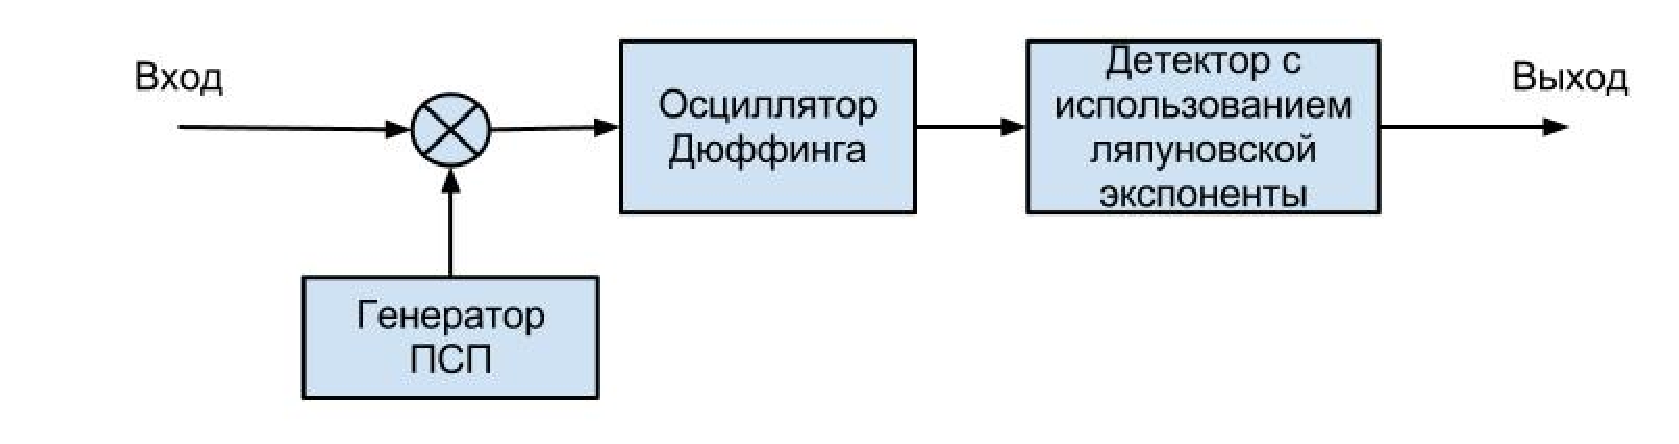
\includegraphics[width=1\linewidth]{Chaos_detector_Lyapunov.eps}}
	\caption{Схема детектора основанного на показателе ляпунова для осциллятора Дуффинга}
	\label{pic:chaos_lyapunov}
\end{figure}

В статье \cite{chaos_chen} предложен усовершенствованный метод, базирующийся на вычислении дисперсии
фазовой траектории. Действительно, на рисунках \ref{pic:duffing_sync}, \ref{pic:duffing_chaos1},
\ref{pic:duffing_chaos2} видно, что когда система находится в хаотическом состоянии значение
дисперсии по координате ${x}$ больше, чем соответствующее значение в состоянии $\omega = \omega_{x}$.
На основе этого была предложена усовершенствованная схема детектора сигнала - рисунок \ref{pic:chaos_energy_detector}
\begin{figure}[H]
	\center\scalebox{0.7}{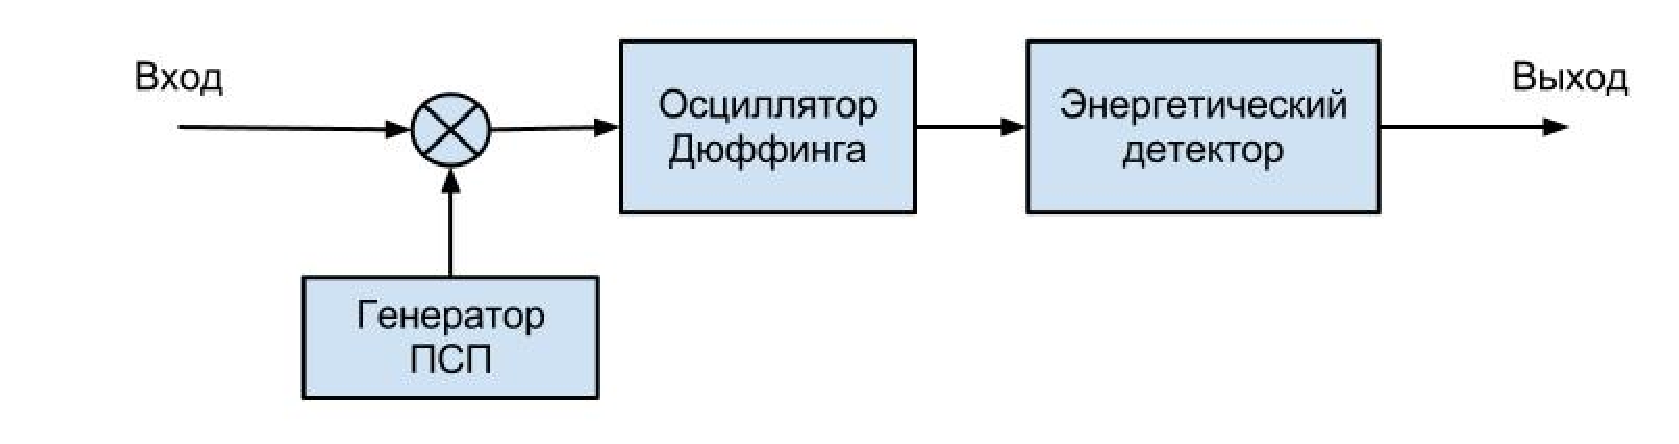
\includegraphics[width=1\linewidth]{chaos_detector.eps}}
	\caption{Схема энергетического детектора для осциллятора Дуффинга}
	\label{pic:chaos_energy_detector}
\end{figure}

%%%%%%%%
% HOS 
Математический аппарат статистик высоких порядков (СВП или HOS - Higher-order statistics)
для исследования непричинных, причинных и нестабильных (систем с неминимальной фазой) и негауссовых сигналов впервые был предложен
в \cite{hos_petropulu} в 1993 году.  Этот метод позволяет не только подавлять цветной Гауссов шум, но так же в некоторых случаях подавлять
цветной не-Гауссов шум.

В работе \cite{hos_zhao} был предложен метод детектирования ШПС с использованием СВП.

%%%%%%%%
% CHE 
Интересная группа алгоритмов основывается на информационной избыточности ШПС, например \cite{phd_che}. В данной
группе алгоритмов используется механизм появления нескольких точек на основном пике КФ, описанный в \cite{kaplan}. Пример
изображен на рисунке \ref{pic:sec1_peak_tcd}.
\begin{figure}[H]
        \center\scalebox{1}{\includegraphics[width=1\linewidth]{corr_peak_tcd.eps}}
        \caption{Идеальная КФ ШПС с отмеченными точками возможного обнаружения}
        \label{pic:sec1_peak_tcd}
\end{figure}
На рисунке \ref{pic:sec1_peak_tcd} изображен пик КФ с несколькими точками. Две точки находятся выше порога ${\Pi=0.5}$.
В работе \cite{phd_che} рассмотрено создание субоптимального обнаружителя на основе информационной избыточности ШПС.
Получена целевая функция системы и намечены дальнейшие пути развития данного направления.

%%%%%%%%
% 2MAX 
Так же одним из направлений исследований является разработка алгоритмов выбора порога без априорной информации о величине ОСШ. Например,
в работах \cite{2max_ieee, 2max_article} представлен алгоритм нахождения пика (АНП) КФ (Peak-finding algorithm).

Данный алгоритм можно разбить на несколько шагов:
\begin{itemize}
\item[Шаг 1] Подсчитать КФ, используя метод предложенный с использованием параллельного коррелятора. 
\item[Шаг 2] Найти главный пик КФ, найти второй пик КФ, найти среднее значение КФ.
\item[Шаг 3] Нормализовать полученные значения относительно главного пика КФ.
\item[Шаг 4] Если (максимум КФ - среднее) > ${\Pi_1}$ и (максимум КФ - 
	второй максимум КФ) > ${\Pi_2}$, тогда полученный главный пик КФ соответствует
	искомой фазе ПСП и частоте.
\end{itemize}

В статье авторов \cite{2max_ieee} предложены следующие значения для порогов:
${\Pi_1} = 0.3$ дБ и  ${\Pi_2} = 0.15$ дБ. Так же авторы предлагают итерационную процедуру для нахождения
фазы ПСП и частоты смещения допплера:
\begin{itemize}
\item[Шаг 1] Начать вычисление с 1мс.
\item[Шаг 2] Получить результаты АНП.
\item[Шаг 3] Если фаза ПСП и частота не могут быть найдены, увеличить время интегрирования сигнала.
	Использовать следующие значения для интегрирования: 1мс -> 10мс -> 50мс -> 100мс -> 200мс ->
	500мс -> 1000мс
\end{itemize}

Очевидным минусом данного подхода является сильная зависимость от интерференции. В городском каньоне будет присутствовать
несколько достаточно мощных лучей, а значит разница в энергии первого и второго пика будет низкой.

%%%%%%
\paragraph{Выводы.}

Во введении кратко приведена история развития СПИ с ШПС, приведены ученые внесшие значительный вклад в разработку данного направления связи. Так же рассмотрена
актуальность исследования в данной области. Кроме того, приведены определения, что такое СПИ с ШПС, ее математическая модель и основные отличительный особенности данного класса систем.
Так же приведены классические и новые подходы к оценке параметров СПИ с ШПС. Рассмотрен оптимальный алгоритм - последовательный коррелятор,
а так же новые достаточно экзотические подходы - применение осциллятора Дуффинга. 

\newpage
 % введение

\addcontentsline{toc}{chapter}{Список сокращений}
\chapter*{Список сокращений}
\noindent
АБГШ - аддитивный белый гауссовский шум				\\
АКП - автокорреляционная последовательность			\\
АКФ – автокорреляционная функция				\\
АНП - алгоритм нахождения пика					\\
АР - авторегрессия						\\
АРСС - авторегрессия скользящего среднего			\\
АЦП - аналогово-цифровой преобразователь			\\
БПФ - быстрое преобразование Фурье				\\
ДПФ - дискретное преобразование Фурье				\\
ДФМ - двоичная фазовая манипуляция				\\
КФ - корреляционная функция					\\
МАВ - максимальная апостериорная вероятность			\\
МНК - метод наименьших квадратов				\\
МШУ - малошумящий усилитель					\\
ОСШ - отношение сигнал-шум 					\\
ПО - программное обеспечение					\\
ПЧ - промежуточная частота					\\
СД - синхронный детектор					\\
СВП - статистики высоких порядков				\\
СНРС - спутниковая навигационная радиоэлектронная система	\\
СНС - спутниковая навигационная система				\\
СКО - средняя квадратическая ошибка				\\
СПМ - спектральная плотность мощности				\\
CC - скользящее среднее						\\
ПСП – псевдослучайная последовательность			\\
УГ - управляемый генератор					\\
ФАП - фазовая автоматическая подстройка				\\
ФАПЧ - фазовая автоподстройка частоты				\\
ФВЧ - фильтр высоких частот					\\
ФНЧ - фильтр низких частот					\\
ФМШПС - фазо-манипупулированный широкополосный сигнал		\\
ЦОС - цифровая обработка сигналов				\\
ШПС -  широкополосные сигналы (шумоподобные сигналы)		\\

\noindent
3G - Third Generation						\\
AGPS - Assisted GPS						\\
BPSK - Binary Phase-Shift Keying				\\
CDMA - Code Division Multiple Access				\\
DAMPS - Digital Advanced Mobile Phone Service			\\
DMA - Delay and Multiply Approach				\\
FTP - file transfer protocol					\\
FPGA - field-programmable gate array 				\\
FPU - floating point unit					\\
GPS - Global Positioning System					\\
GSM - Global System for Mobile Communications (ранее Groupe Spécial Mobile) \\
HOS - Higher-order statistics					\\
NWPR - Narrowband-Wideband Power Ratio				\\
RAM - random access memory					\\
RFID - Radio Frequency IDentification				\\
RSCN - Real Signal-Complex Noise				\\
SDK - Software Development Kit					\\
SDR - Software Defined Receiver					\\
SNV - Signal-to-Noise Variance					\\
SNR - Signal-to-Noise Rate					\\
VHDL - VHSIC ((Very high speed integrated circuits) Hardware Description Language			\\
WAAS - Wide Area Augmentation System				\\


\clearpage
		% acronyms 
\addcontentsline{toc}{section}{СПИСОК УСЛОВНЫХ ОБОЗНАЧЕНИЙ}
\section*{СПИСОК УСЛОВНЫХ ОБОЗНАЧЕНИЙ}
${E[X]}$ - математическое ожидание случайной величины $X$	\\
${D[X]}$ - дисперсия случайной величины $X$			\\
${r_{xx}(\tau)}$ - АКП для смещения ${\tau}$			\\
${\bf{R_M}}$ - автокорреляционная матрица			\\
\newpage
		% definitions

\addcontentsline{toc}{section}{ВВЕДЕНИЕ}
\section*{ВВЕДЕНИЕ}

Большое количество современных систем являются беспроводными. Простота развертывания, мобильность, относительно низкая
стоимость - вот основные преимущества беспроводных систем. Количество мобильных устройств (телефоны, планшетные компьютеры
и т.д.) с каждым годом стремительно растет, только мобильных телефонов в 2011 году было 5.6 миллиарда и покрывало 79.86\%
\cite{wiki_mobilenum} населения земли. Технологии беспроводной связи глубоко проникли во все сферы жизни общества:
обеспечение безопасности с помощью RFID датчиков, предоставление доступа в интернет по технологиями 3G, WiFi, 
сотовая связь по различным технологиям (GSM, CDMA, DAMPS). Некоторые из этих систем строятся на основе методики
расширения спектра, которая отвечает современным требованиям по мощности сигнала, а так же по безопасности передаваемых
данных. В основе таких систем лежат шумоподобные (широкополосные) сигналы - ШПС. Вместе с тем растут требования к таким
системам. Применение ШПС ставит ряд специфических задач по обработке информации, обусловленных особенностями ШПС.
Свойства характерные для ШПС, выгодно отличают данный класс систем от класса узкополосных систем, но с другой стороны
оборачивается усложнением методов обработки ШПС.

Внедрение новых технологий требует увеличение полосы частот. Разнообразие технологий беспроводной передачи данных среди
гражданских и военных систем ведет к перегрузке каналов связи и все более высоким требованиям к скорости передачи
данных. С учётом данных требований применение систем передачи информации с ШПС становится все более востребованным.

Принимая во внимание географические размеры России и стратегическую важность обладания собственными системами спутникового
позиционирования, правительство Российский Федерации уделяет особое внимание разработке собственной системы
глобального спутникового позиционирования ГЛОНАСС. Обладание собственными технологиями системы спутниковой навигации (СНС), государство может обезопасить
себя в случае военных конфликтов от ограничения применения американской системы СНС Navstar GPS в зоне конфликта.

Разработка систем, позволяющих работать с несколькими различными СНС, позволит повысить точность определения координат
в сложных условиях города. Сложность детектирования сигнала и определения координат обусловлена наличием плотной
застройки многоэтажными зданиями. В городских условиях задача подавления интерференционной помехи становится особенно
актуальной. Спектр интерференционной помехи не является белым, а фильтрация и компенсация цветного шума
требует разработки специальных алгоритмов.

Новые цифровые процессоры позволяют применять подходы, которые еще 10-15 лет назад были бесперспективными.
В данной работе развиваются подходы на основе построения параметрической модели ШПС. Невозможность использования
методов требующих вычислений с высокой точностью в приемниках реального времени
10-15 лет назад была обусловлена слабой производительностью процессоров и микроконтроллеров, а так же существенной
стоимостью процессоров с модулем для операций с числами с плавающей точкой. Современное развитие цифровых технологий делает 
возможным применение параметрических методов оценки спектра взамен традиционного подхода основанного на непараметрического
анализа спектра.

Основа теории систем связи с ШПС была заложена в работах В.А. Котельникова и К. Шеннона.
России в этой области занимались В.И. Борисов, В.Б. Пестряков, В.И. Журавлев, М.И. Жодзишский, Б.И. Шахтарин, Л.Е.  Варакин, В.Е. Гантмахер и др.

Изначально методы расширенного спектра применялись при разработке военных систем управления и связи \cite{sklyar}.
К концу второй мировой войны расширение спектра применялось в радиолокации для борьбы с преднамеренными помехами, а
в последствии развитие данной технологии объяснялось желанием создать помехоустойчивые системы связи.
В конце 40-х-начале 50-х годов прошлого века Мортимер Рогофф, сотрудник Международной Телефонной и Телеграфной Корпорации (США) (ITT),
провёл эксперимент по передаче информации при помощи псевдошумового сигнала \cite{sklyar}, среди отечественных ученых
в середине 30-х годов прошлого века работу об основах кодового разделения каналов написал Д.В. Агеев.
Первые разработки таких систем относились к военным отраслям. Данный факт объясняется рядом особенностей, которыми обладают
сигналы с расширенным спектром, в числе которых — сложность перехвата заложенной в них информации,
высокая помехоустойчивость, а также трудность обнаружения факта работы передатчика. В процессе исследований расширенному спектру
нашлось и другое применение - снижение плотности энергии, высокоточная локация, использование при множественном доступе
\cite{sklyar}

Системы связи с широкополосными сигналами занимают особое место. Их особенные свойства выделяют данный класс из других систем
связи. Высокая помехозащищенность при действии сильной помехи, кодовое разделение большого количества абонентов, прием
информации с высокой достоверностью - отличительные особенности широкополосных система. Эти черты были известно, но
уровень элементной базы и низкий уровень помех не позволяли получить развития системам данного класса. Однако развитие
элементной привело к широкому распространению данного вида сигналов. В настоящее они применяются в системах спутниковой навигации,
системах сотовой связи и др \cite{varakin-book}.

Отношение сигнал/шум (ОСШ) на входе приемника может быть очень низким. Для обеспечения высокой помехозащищенности 
в таких случаях используются ШПС с большими и сверхбольшими базами.

К созданию сложных широкополосных сигналов (СШС) привело решение ряда проблем при развитии систем передачи данных.
Первая проблема встала при разработке новых радиолокационных система. Для дальнейшего развития требовалось
решить несколько противоречий: требование высокой разрешающей способности по дальности и дальностью обнаружения
целей в импульсных РЛС, требование точного измерения скорости и высокое разрешение по дальности, требование
увеличить дальность при ограничении пиковой мощности \cite{gantmaher-book}. Решение данных задач было предложено
Ф. Вудвардом. Им было показано, что дополнительным параметром является форма сигнала. Длительность сигнала
может быть больше - настолько больше, насколько это необходимо для обеспечения энергетических требований, а требование
разрешения по дальности и точности измерений определяются шириной полосы сигнала. Данные требования обеспечивается
путем сжатия импульса на стороне приемника. Вудворд сформулировал принципы: произведение эффективной полосы частот
радиосигнала на его длительность должен быть существенно больше единиц ${FT>>1}$, внутренняя структура сигнала
должна быть такой, чтобы обеспечить возможность приемнику сжатие распределенного во времени сигнала в короткий импульс,
соответствующий полосе ${F}$ \cite{gantmaher-book}.

В \cite{gantmaher-book} показана связь пропускной способности канала с понятием ШПС. При ${R_e<<1}$ можно записать:
\begin{center}
\begin{equation}
	\label{eq:shennon_cdma}
	FT = \frac{1}{\log(1+R_e)},
\end{equation}
\end{center}
где ${R_e}$ - ОСШ, ${F}$ - эффективная полоса частот, ${T}$ - длительность.

Стоить отметить, что при ${R_e<<1}$, левая часть выражения \ref{eq:shennon_cdma} стремится к бесконечности, а значит
ШПС позволяет обеспечить теоретически неограниченную достоверность передачи информации. Второе важное свойство
ШПС, следующее из \ref{eq:shennon_cdma} - способность работать "под шумами". Что обеспечивает скрытность
передачи информации, а с другой высокую степень уплотнения каналов связи и, как следствие, решение современных проблем
с перегруженностью каналов связи.

В данной работе будет рассматриваться ШПС модулированный ПСП на основе двоичной рекуррентной последовательности.
Для выделения данных из потока необходимо иметь точно синхронизированную копию ПСП, которая была использована
при модулировании сигнала на передающей стороне. Для достижения синхронизма на стороне приемника необходимо
устранить неопределенность в двух областях: неопределенность по частоте и неопределенность по фазе (задержке) ПСП.
Неопределенность по фазе ПСП обусловлена неопределенностью в расстоянии между передатчиком и приемником. Неопределенность
по частоте обусловлена в первую очередь допплеровским эффектом, а так же нестабильностью опорных генераторов в
передатчике и приемнике. После устранения неопределенности по частоте для достижения точной синхронизации
начинается процесс слежения за частотой. Неопределенность по фазе ПСП устранить, не используя полный перебор,
невозможно в силу корреляционных свойств ПСП. Таким образом можно заключить, что задача быстрого и эффективного
поиска и оценки параметров ШПС является актуальной.

В данной работе рассматривается подход программного приемника (Software Defined Receiver - SDR)
\cite{akos-book, grayver-book, pany-book} для оценки параметров ШПС. Как уже было отражено выше, ШПС применяется во
многих системах. В данной работе для полунатурного эксперимента будет рассматриваться сигнал СНС Navstar GPS. Данная система передачи 
информации использует ПСП Голда \cite{gold-ieee} для модулирования сигнала.

Традиционные подходы к реализации приемника СНС Navstar GPS отражены в \cite{akos-book, tsui}. 

Популярность и распространенность данной системы стимулирует исследования в области детектирования
и оценки частоты ШПС сигналов.

Существуют исследования в области применения теории хаоса - детектирование и оценка
частоты ШПС с применением осциллятора Дуффинга \cite{chaos_cambridge, chaos_chen, chaos_huang, chaos_wang}. Преимуществом
данного подхода является то, что свойства осциллятора позволяют детектировать сигналы с экстремально низким ОСШ. В то же
время, на данный момент никто не предложил цифровое представление осциллятора Дуффинга, а это затрудняет использование данного подхода
в реальных приемниках. Таким образом данное направление является в настоящее время больше теоретическим, чем практическим.

В работах \cite{hos_petropulu, hos_zhao} предложено использовать статистики высоких порядков для подавления шума и детектирование
сигналов с низким уровнем ОСШ.

Более традиционные подходы для детектирования и оценки параметров ШПС сигналов с низким уровнем ОСШ рассмотрены в монографии \cite{ziedan-book}.
В данной монографии рассматриваются как методы детектирования и оценки параметров ШПС, основанные на когерентном накоплении, так и эффективные
системы слежения за частотой и фазой ПСП.

{\bf{Добавить ЦЕЛИ И ЗАДАЧИ}}

%%%%%%
\paragraph{Постановка задачи оценки параметров сигнала с расширенным спектром.}
В данной работе рассматриваются задачи повышения рабочих характеристик приемников ШПС, поэтому целесообразно отразить основные модули этой системы 
на примере СНС Navstar GPS - рисунок \ref{pic:sec1_gnss_system}.
\begin{figure}[H]
\center\scalebox{1}{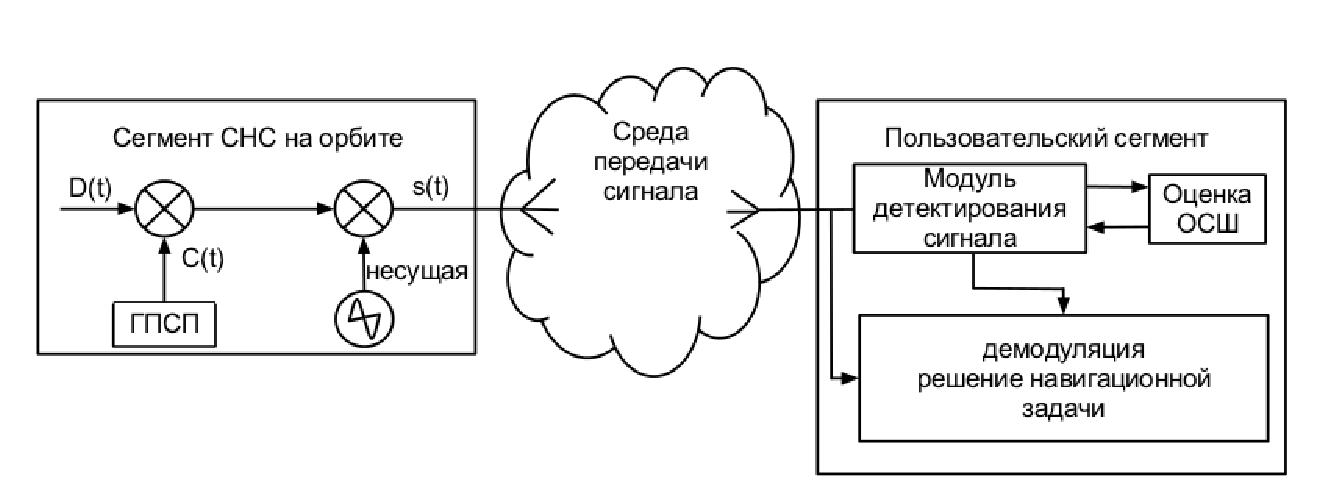
\includegraphics[width=1\linewidth]{sec1gnss_system.eps}}
\caption{структутраная схема СНС GPS}
\label{pic:sec1_gnss_system}
\end{figure}

В систему СНС Navstar GPS входят космический сегмент, наземный сегмент (на рисунке \ref{pic:sec1_gnss_system} не
отражен), а так же пользовательский сегмент. В космический сегмент входит спутниковая группировка, в 
наземный - станции управления, в пользовательский - все устройства принимающие сигнал от СНС GPS.

\paragraph{Модель сигнала и помех.}
В системе СНС Navstar GPS применяется ШПС.
Система передачи информации считается системой с расширенным спектром в следующих случаях \cite{sklyar}:
\begin{enumerate}
	\item Используемая полоса значительно шире минимальной, необходимой для передачи данных.
	\item Расширение спектра производится с помощью так называемого расширяющего сигнала (ПСП),
		который не зависит от передаваемой информации.
	\item Восстановление исходных данных ("сужение спектра") осуществляется путем сопоставления полученного
		сигнала и синхронизированной копии расширяющего сигнала (ПСП)
\end{enumerate}

Так же подобные сигналы называют:
\textquotedblleftсложными\textquotedblright,
\textquotedblleftшумоподобными\textquotedblright,
\textquotedblleftпсевдослучайными\textquotedblright,
\textquotedblleftсложными-дискретными\textquotedblright,
\textquotedblleftдискретно-кодированными\textquotedblright,
\textquotedblleftортогональными (квазиортогональными)\textquotedblright,
\textquotedblleftоптимальными дискретными\textquotedblright
\cite{gantmaher-book}.

Каждое название ставит акцент на определенной характеристике сигнала. В данной работе я буду оперировать термином
широкополосный сигнал - ШПС. ШПС можно определить как \cite{gantmaher-book, varakin-book}:
\begin{center}
\begin{equation}
	\label{eq:ss_signal}
	1 << FT = B,
\end{equation}
\end{center}
где: ${B}$ - база сигнала, ${F}$ - эффективная ширина спектра, а ${T}$ - длительность.
Неточность этого определения рассмотрена в \cite{gantmaher-book}, так же там даны ссылки на другие источники
разделяющие критику данного определения. Для данной работы критика, рассмотренная в приведенных источниках,
принципиального значения не имеет.

%%%%%%
\paragraph{Классическая постановка задачи оценки параметра.}
Из литературы по теории автоматических систем, например \cite{pugachev} (глава 10.1), известна классическая постановка
задачи задачи теории оптимальных систем. "На практике часто приходится решать задачу проектирования системы, когда
требуется определить характеристики системы таким образом, чтобы она имела наибольшую точность при данных условиях.
Систему обеспечивающую наибольшую возможную точность с какой-нибудь определенной точки зрения среди всех систем
заданного класса, обычно называют оптимальной" \cite{pugachev}.

В одной из постановок данной задачи \cite{pugachev} (глава 10.1), система считается полностью неизвестной
и требуется определить ее оператор так, чтобы она была оптимальной с точки зрения принятого критерия качества. Эта
задача сводится к определению с наибольшей возможной точностью некоторых параметров, от которых зависит принимаемый
сигнал. Но при этом важно учитывать не только точность, но и другие факторы, так как проектируемая система должна
удовлетворять многим, часто противоречивым требованиям. В виду приведенных факторов, обычно представляет собой
ряд компромиссных решений, удовлетворяющих всем предъявляемым к системе требованиям.

Точность автоматической системы обычно характеризуется математическим ожиданием и дисперсией ее ошибки.
Математическое ожидание представляет собой систематическую ошибку системы в данных условиях, а дисперсия
характеризует уровень случайных ошибок \cite{pugachev} (глава 10.2). Так как в различных условиях работы
системы, которые встречаются случайно систематическая ошибка тоже является случайной, за критерий качества
системы при ее проектировании обычно принимают второй начальный момент ошибки - математическое ожидание
квадрата ошибки:
\begin{center}
\begin{equation}
	\label{eq:stat_err_prob}
	\eta = M[e^2(t)]
\end{equation}
\end{center}
Положительный квадратный корень из этой величины называют средней квадратичной ошибкой системы. Таким образом,
оптимальной системой обычно считают такую систему, которая имеет минимальную среднюю квадратичную ошибку.

Критерий минимума средней квадратичной ошибки является простейшим с математической точки зрения и обычно приводит
к наиболее простым методам определения оптимальных систем. Однако далеко не во всех задачах он может служить мерой
качества системы. Поэтому нельзя ограничиваться методами нахождения оптимальных систем по критерию минимума средней
квадратичной ошибки.

В случаях, когда необходимо проектировать следящую систему, приходится учитывать возможность срыва слежения,
который заключается в том что система перестает работать, если ее ошибка превосходит по абсолютной величине некоторый
уровень. При проектировании таких систем целесообразно принять за критерий качества вероятность срыва слежения. При
этом оптимальной считается такая система, которая обеспечивает минимум вероятности срыва слежения. Если срыв слежения
происходит в случае, когда абсолютная величина ошибки превосходит уровень $a$, то критерий минимума вероятности ошибки
слежения можно представить \cite{pugachev} (глава 10.2):
\begin{center}
\begin{equation}
	\label{eq:prob_lost_signal}
	p = P(e(t) > a) = min
\end{equation}
\end{center}

%%%%%%
\paragraph{Введение обозначений.}
В диссертации рассматривается сигнал с расширенным спектром полученный методом "прямой последовательности".
Данный метод заключается в том, что гармоническая несущая сигнала модулируется высокоскоростным (широкополосным)
расширяющим сигналом (ПСП). 

Несущее колебание с частотой ${\omega_0}$  модулируется данными ${d(t)}$ , а также высокоскоростной ПСП ${g(t)}$, полученной методом "прямой последовательности".
СПИ Navstar GPS осуществляется двоичная фазовая модуляция (ДФМ или 2-ФМ), а значит ${d(t)}$  и ${g(t)}$  - потоки антиподных импульсов \{-1, 1\}.
Таким образом сигнал на выходе модулятора может быть представлен \cite{shahtarin_sync}:
\begin{equation}
	\label{eq:cdma_eq}
	s(t)=Ad(t)g(t)\cos{(\omega_{0}t)},
\end{equation}
где ${d(t)}$- информационный бит, а ${g(t)}$ - ПСП представляет собой фазовый сдвиг  ${0, \pi}$.

В реальных СПИ сигнал на приемник поступает одновременно от нескольких источников, присутствует неопределенность по частоте, а также аддитивный белый шум (АБГШ).
В приемнике после оцифровки сигнала получаем смесь:
\begin{equation}
	\label{eq:cdma_strip_eq}
	x(m)=\sum_{k=1}^{N}\left( A_k g(m + \tau_k)\exp{\left[j \left( \tilde{\omega}_{k}m + \phi_k(m)\right)\right]} \right) + n(m),
\end{equation}
где  ${k}$ - относительный номер источника сигнала, ${N}$ - количество доступных источников сигнала, модулированных ПСП одного семейства,
${m}$ - индекс соответствующий времени, ${\tilde{\omega}_{k}}$  – относительная частота, соответствующая ${\omega_0}$,
${\tau_k}$ - задержка модулирующей ПСП в точке приема, ${\phi_k(m)}$ - случайная начальная фаза, ${n(m)}$ - аддитивный белый гауссов шум (АБГШ). 

Следует отметить, что при оценке фазы сигнала с номером ${k}$  интерференцией являются сигналы:    .
\begin{equation}
	%\label{eq:cdma_interference}
	\{n \ne k, n \in [1,N]\}
\end{equation}

%%%%%%
\paragraph{Алгоритмы оценки параметров широкополосного сигнала сигнала.}
Алгоритм реализующий метод максимального правдоподобия - последовательный коррелятор. Данный подход реализуется в аппаратных приемниках.
Аппаратный приемник позволяет реализовать параллельно несколько последовательных корреляторов и вести оценку параметров
СПИ с ШПС параллельно.

Данный алгоритм в некоторых источниках так же называется согласованным фильтром. В \cite{sklyar} рассмотрены нюансы этих двух понятий.
В данной работе используется понятие последовательный коррелятор. Работа коррелятора описывается математической операцией
корреляции \ref{eq:serial_corr}. Сигнал коррелируется с локальной копией и на выходе коррелятора получается значение, отражающее
степень совпадения сигналов. Не трудно представить, что сигнал с хорошими корреляционными свойствами должен обладать высоким значением
корреляции когда сигналы синхронизированы и минимальным значением в любом другом случае (фаза ПСП не выровнена - отсутствие сигнала).
\begin{equation}
	\label{eq:serial_corr}
	y(n)=\sum\limits_{m=0}^{N-1}{x(m)h(n+m)},
\end{equation}
где ${x(m)}$ - принятая смесь, а ${h(n)}$ не импульсная характеристика системы, а локальная копия сигнала.

%%%%%%%%
% DFT

Вычисление циклической свертки через дискретное преобразование Фурье (ДПФ) - достаточно популярный метод
в программных приемниках, так как позволяет существенно уменьшить количество операций при вычислении. Но, как показано
в \cite{tsui, oppenheim}, можно достаточно просто перейти от свертки к циклической корреляции. Так как этот метод является самым
популярным в программных приемниках стоит его представить.
Свертка может быть представлена как:
\begin{equation}
	\label{eq:fft_conv}
	y(n)=\sum\limits_{m=0}^{N-1}{x(m)h(n-m)}
\end{equation}

Стоит отметить, что в \ref{eq:fft_conv} сдвиг во времени является циклическим, поскольку дискретные операции являются циклическими.
Возьмем ДПФ от \ref{eq:fft_conv}
\begin{center}
\begin{eqnarray}
	\label{eq:fft_conv_fft}
	Y(k) & = & \sum\limits_{n=0}^{N-1}\sum\limits_{m=0}^{N-1}{x(m)h(n-m)e^{(-j2\pi{kn})/N}}=\nonumber \\
	& = & \sum\limits_{m=0}^{N-1}{x(m)}[\sum\limits_{n=0}^{N-1}h(n-m)e^{(-j2\pi{(n-m)}k)/N}]e^{(-j2\pi{m}k)/N}=\\
	& = & H(k)\sum\limits_{m=0}^{N-1}e^{(-j2\pi{m}k)/N} = X(k)H(k)\nonumber 
\end{eqnarray}
\end{center}
Из уравнения \ref{eq:fft_conv_fft} легко видеть, что это не линейная свертка. В линейной свертке для входного сигнала размером в ${N}$ точек,
результат будет из ${2N-1}$ точек. А в уравнении выше, результатом является всего ${N}$ точек.
Это проявление циклической природы ДПФ.

Алгоритм оценки не использует свертку, он использует корреляцию, которая отличается от свертки. Корреляция
между $x(n)$ и $h(n)$ записывается выражением \ref{eq:serial_corr}:
Единственным отличаем между \ref{eq:serial_corr} и \ref{eq:fft_conv} является знак перед $m$ в ${h(n+m)}$.
В случае оценки параметра ШПС, $h(n)$ является локальной копией сигнала, а не импульсной характеристикой.
Произведем ДПФ над $z(n)$:
\begin{center}
\begin{eqnarray}
	\label{eq:fft_corr_fft}
	Z(k) & = & \sum\limits_{n=0}^{N-1}\sum\limits_{m=0}^{N-1}{x(m)h(n+m)e^{(-j2\pi{kn})/N}}=\nonumber \\
	& = & \sum\limits_{m=0}^{N-1}{x(m)}[\sum\limits_{n=0}^{N-1}h(n+m)e^{(-j2\pi{(n+m)}k)/N}]e^{(j2\pi{m}k)/N}=\\
	& = & H(k)\sum\limits_{m=0}^{N-1}e^{(j2\pi{m}k)/N} = X(k)H^{-1}(k)\nonumber 
\end{eqnarray}
\end{center}
где ${X^{-1}(k)}$ - обратное ДПФ. Уравнение \ref{eq:fft_corr_fft} можно записать как:

\begin{equation}
	\label{eq:fft_corr_fft_rev}
	Y(k) = \sum\limits_{n=0}^{N-1}\sum\limits_{m=0}^{N-1}{x(n+m)h(m)e^{(-j2\pi{kn})/N}}=X^{-1}(k)H(k)
\end{equation}

Если сигнал $x(n)$ действительный, то $x(n) = x^*(n)$, где ${^*}$ - операция комплексного сопряжения. Используя данное соотношение,
значение $Z(k)$ может быть записано:
\begin{equation}
	\label{eq:fft_magnitude}
	|Z(k)|=|H^*(k)X(k)|=|H(k)X(k)^*|
\end{equation}
Данное соотношение может быть использовано для нахождения значения циклической корреляции между входным сигналом и 
локальной копией.

%%%%%%%%
% Chaos 
Оценка параметров СПИ с ШПС (в частности сигналов системы Navstar GPS) с помощью осциллятора Дуффинга
достаточно новое направление в исследованиях по данной тематике. В данной области опубликовано несколько работ, в частности \cite{chaos_chen, chaos_cambridge, chaos_huang, chaos_song}.
Так же является интересной более ранняя статья не рассматривающая GPS \cite{chaos_wang}.
Осциллятор Дуффинга с гармоническим внешним воздействием может быть описан уравнением:
\begin{center}
\begin{equation}
	\label{eq:duffing}
	mx'' + cx' + k_{1}x + k_{2}x^3 = F_{0}\cos(\omega{t}),
\end{equation}
\end{center}
где $m$ - масса, $c$ - коэффициент диссипации, $x$ - состояние осциллятора, $k_1$ и $k_2$ - линейный и нелинейный коэффициенты соответственно,
$F_{0}\cos(\omega{t})$ - внешнее воздействие.

Подробно уравнение \ref{eq:duffing} рассмотрено в \cite{chaos_neimark_landa}.
Для использования осциллятора Дуффинга с целью оценки параметров ШПС была предложена усовершенствованная форма \cite{chaos_song, chaos_chen}:
\begin{center}
\begin{equation}
	\label{eq:duffing_gps}
	x'' +cx' - x^3 + x^5 = \gamma\cos(\omega{t}) + (\gamma_{x}\cos(\omega_{x}) + n(t))
\end{equation}
\end{center}

Перепишем динамическую систему \ref{eq:duffing_gps} в виде:
\begin{center}
\begin{equation}
	\label{eq:duffing_gps_2}
	\left\{
	\begin{aligned}
		y(t) & = x'(t) \\
		y'(t) & =  -cx' + x^3 - x^5 + \gamma\cos(\omega{t}) + (\gamma_{x}\cos(\omega_{x}) + n(t)),
	\end{aligned}
	\right.
\end{equation}
\end{center}
где ${n(t)}$ - АБГШ.

Пример фазового портрета при ${\omega=\omega_{x}}$ изображен на рисунке \ref{pic:duffing_sync},
фазовый портрет хаоса расположен на рисунках \ref{pic:duffing_chaos1}, \ref{pic:duffing_chaos2}
\begin{figure}[H]
	\center\scalebox{0.5}{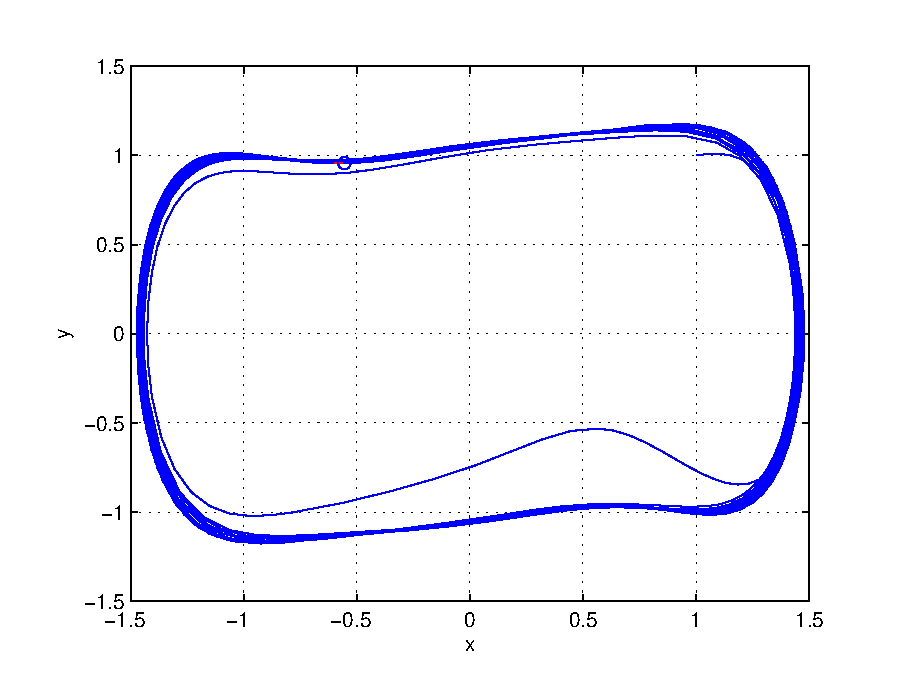
\includegraphics[width=1\linewidth]{duffing_sync.eps}}
	\caption{Фазовый портрет при ${\omega =\omega_{x}}$}
	\label{pic:duffing_sync}
\end{figure}
\begin{figure}[H]
	\center\scalebox{0.5}{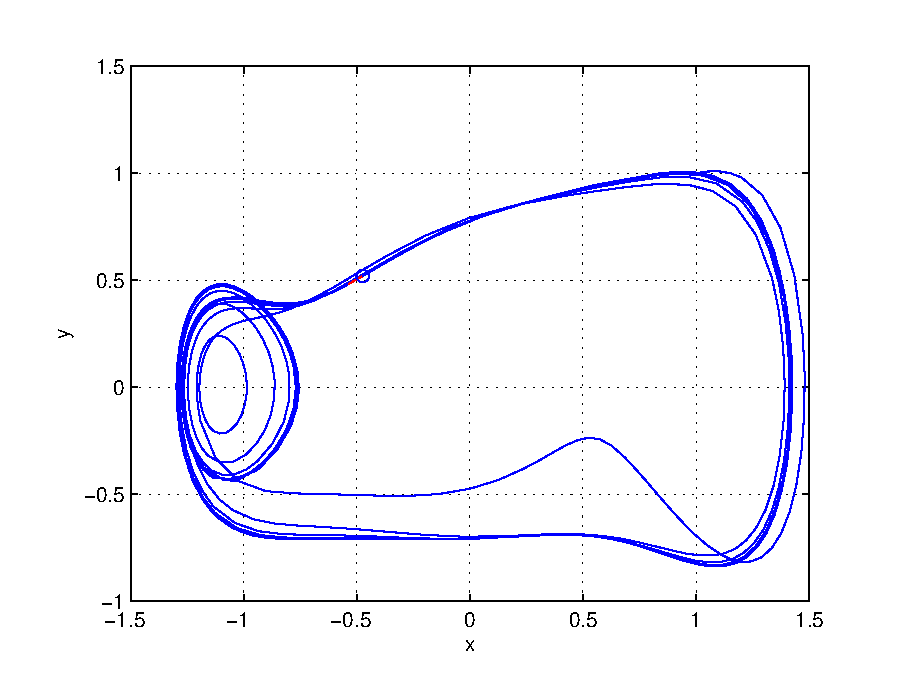
\includegraphics[width=1\linewidth]{duffing_chaos1.eps}}
	\caption{Фазовый портрет при ${\omega < \omega_{x}}$}
	\label{pic:duffing_chaos1}
\end{figure}
\begin{figure}[H]
	\center\scalebox{0.5}{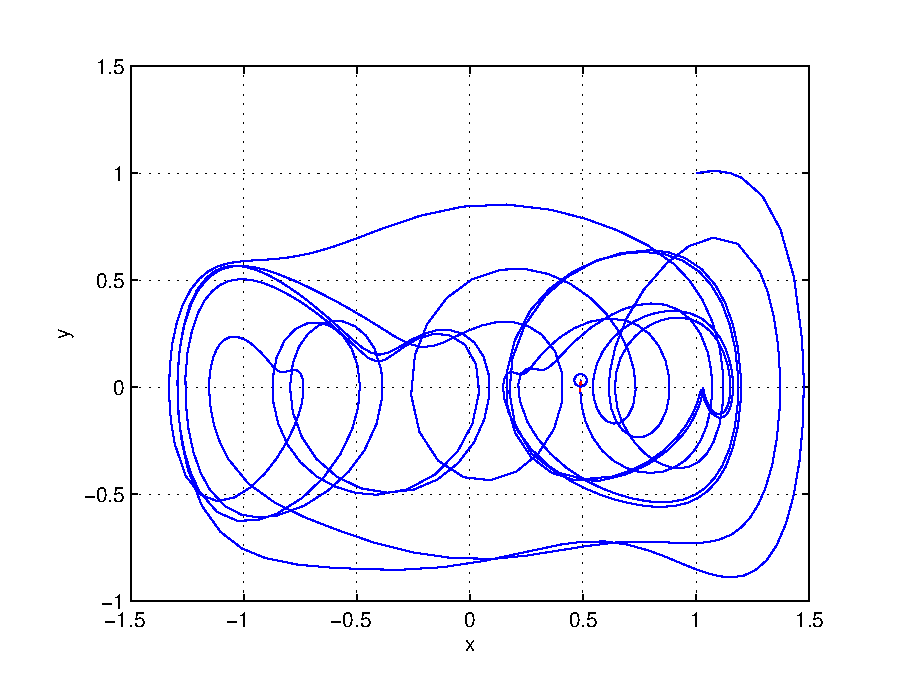
\includegraphics[width=1\linewidth]{duffing_chaos2.eps}}
	\caption{Фазовый портрет при ${\omega > \omega_{x}}$}
	\label{pic:duffing_chaos2}
\end{figure}
В качестве параметров уравнения применялись: $c = 0.5$, $\gamma=\gamma_{x}=0.36$, ${\omega=1}$

Часто для вычисления характеристик хаотической динамики применяется показатель Ляпунова.
Он показывает в каком состоянии находится система. Если система находится
в стабильном состоянии линии фазовой траектории будут близко прилегать одна к другой, в противном
случае система находится в состоянии хаоса. Детектор с применением показателя Ляпунова
представлен на рисунке \ref{pic:chaos_lyapunov}.
\begin{figure}[H]
	\center\scalebox{0.7}{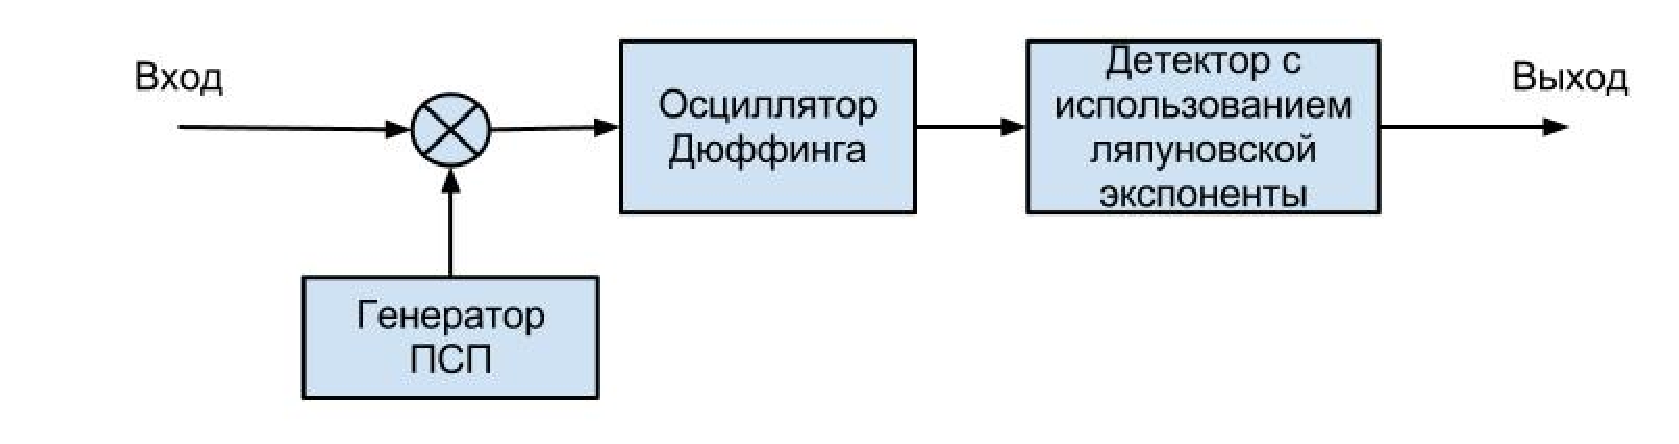
\includegraphics[width=1\linewidth]{Chaos_detector_Lyapunov.eps}}
	\caption{Схема детектора основанного на показателе ляпунова для осциллятора Дуффинга}
	\label{pic:chaos_lyapunov}
\end{figure}

В статье \cite{chaos_chen} предложен усовершенствованный метод, базирующийся на вычислении дисперсии
фазовой траектории. Действительно, на рисунках \ref{pic:duffing_sync}, \ref{pic:duffing_chaos1},
\ref{pic:duffing_chaos2} видно, что когда система находится в хаотическом состоянии значение
дисперсии по координате ${x}$ больше, чем соответствующее значение в состоянии $\omega = \omega_{x}$.
На основе этого была предложена усовершенствованная схема детектора сигнала - рисунок \ref{pic:chaos_energy_detector}
\begin{figure}[H]
	\center\scalebox{0.7}{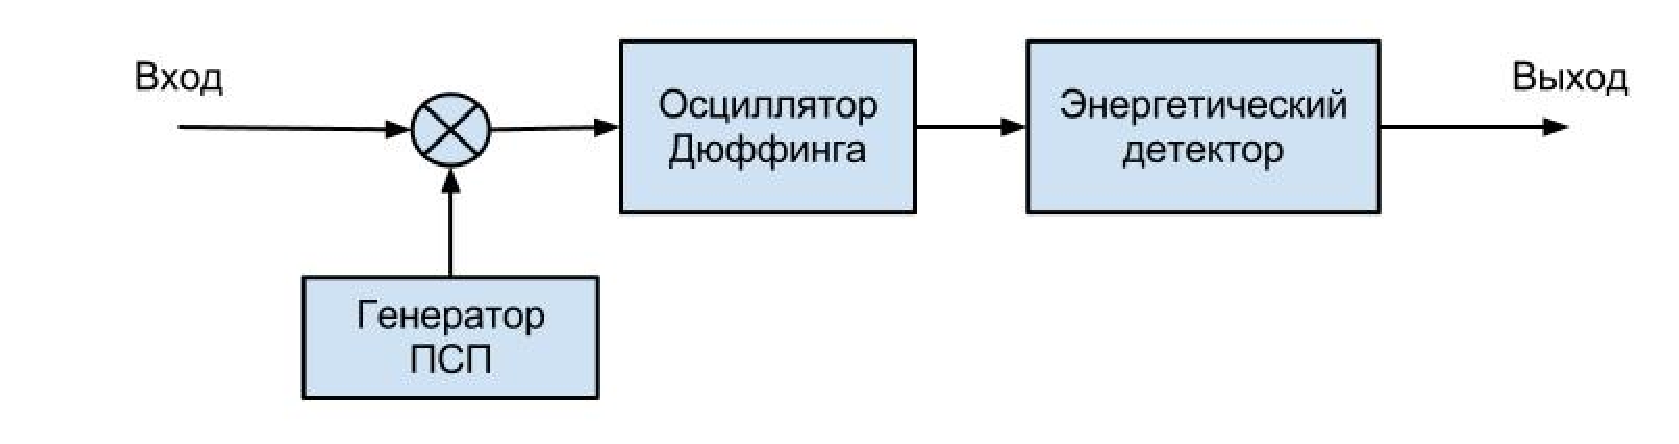
\includegraphics[width=1\linewidth]{chaos_detector.eps}}
	\caption{Схема энергетического детектора для осциллятора Дуффинга}
	\label{pic:chaos_energy_detector}
\end{figure}

%%%%%%%%
% HOS 
Математический аппарат статистик высоких порядков (СВП или HOS - Higher-order statistics)
для исследования непричинных, причинных и нестабильных (систем с неминимальной фазой) и негауссовых сигналов впервые был предложен
в \cite{hos_petropulu} в 1993 году.  Этот метод позволяет не только подавлять цветной Гауссов шум, но так же в некоторых случаях подавлять
цветной не-Гауссов шум.

В работе \cite{hos_zhao} был предложен метод детектирования ШПС с использованием СВП.

%%%%%%%%
% CHE 
Интересная группа алгоритмов основывается на информационной избыточности ШПС, например \cite{phd_che}. В данной
группе алгоритмов используется механизм появления нескольких точек на основном пике КФ, описанный в \cite{kaplan}. Пример
изображен на рисунке \ref{pic:sec1_peak_tcd}.
\begin{figure}[H]
        \center\scalebox{1}{\includegraphics[width=1\linewidth]{corr_peak_tcd.eps}}
        \caption{Идеальная КФ ШПС с отмеченными точками возможного обнаружения}
        \label{pic:sec1_peak_tcd}
\end{figure}
На рисунке \ref{pic:sec1_peak_tcd} изображен пик КФ с несколькими точками. Две точки находятся выше порога ${\Pi=0.5}$.
В работе \cite{phd_che} рассмотрено создание субоптимального обнаружителя на основе информационной избыточности ШПС.
Получена целевая функция системы и намечены дальнейшие пути развития данного направления.

%%%%%%%%
% 2MAX 
Так же одним из направлений исследований является разработка алгоритмов выбора порога без априорной информации о величине ОСШ. Например,
в работах \cite{2max_ieee, 2max_article} представлен алгоритм нахождения пика (АНП) КФ (Peak-finding algorithm).

Данный алгоритм можно разбить на несколько шагов:
\begin{itemize}
\item[Шаг 1] Подсчитать КФ, используя метод предложенный с использованием параллельного коррелятора. 
\item[Шаг 2] Найти главный пик КФ, найти второй пик КФ, найти среднее значение КФ.
\item[Шаг 3] Нормализовать полученные значения относительно главного пика КФ.
\item[Шаг 4] Если (максимум КФ - среднее) > ${\Pi_1}$ и (максимум КФ - 
	второй максимум КФ) > ${\Pi_2}$, тогда полученный главный пик КФ соответствует
	искомой фазе ПСП и частоте.
\end{itemize}

В статье авторов \cite{2max_ieee} предложены следующие значения для порогов:
${\Pi_1} = 0.3$ дБ и  ${\Pi_2} = 0.15$ дБ. Так же авторы предлагают итерационную процедуру для нахождения
фазы ПСП и частоты смещения допплера:
\begin{itemize}
\item[Шаг 1] Начать вычисление с 1мс.
\item[Шаг 2] Получить результаты АНП.
\item[Шаг 3] Если фаза ПСП и частота не могут быть найдены, увеличить время интегрирования сигнала.
	Использовать следующие значения для интегрирования: 1мс -> 10мс -> 50мс -> 100мс -> 200мс ->
	500мс -> 1000мс
\end{itemize}

Очевидным минусом данного подхода является сильная зависимость от интерференции. В городском каньоне будет присутствовать
несколько достаточно мощных лучей, а значит разница в энергии первого и второго пика будет низкой.

%%%%%%
\paragraph{Выводы.}

Во введении кратко приведена история развития СПИ с ШПС, приведены ученые внесшие значительный вклад в разработку данного направления связи. Так же рассмотрена
актуальность исследования в данной области. Кроме того, приведены определения, что такое СПИ с ШПС, ее математическая модель и основные отличительный особенности данного класса систем.
Так же приведены классические и новые подходы к оценке параметров СПИ с ШПС. Рассмотрен оптимальный алгоритм - последовательный коррелятор,
а так же новые достаточно экзотические подходы - применение осциллятора Дуффинга. 

\newpage


% sec 1
\section{Постановка задачи детектирования фазоманипулированного сигнала с расширенным спектром}
\label{sec1_acq_algo}

\subsection{Постановка задачи поиска сигнала}
В данной работе рассматриваются задачи повышения рабочих характеристик приемников cпутниковой навигационной системы
(СНС) GPS, поэтому целесообразно
отразить основные модули этой системы рисунок \ref{pic:sec1_gnss_system}.
\begin{figure}[H]
\center\scalebox{1}{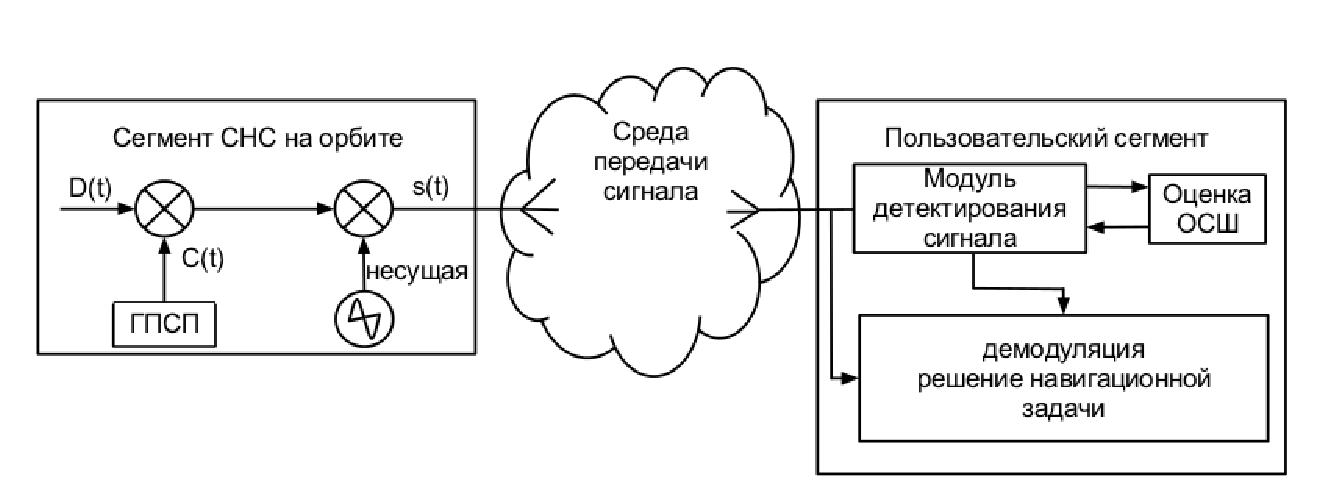
\includegraphics[width=1\linewidth]{sec1gnss_system.eps}}
\caption{структутраная схема СНС GPS}
\label{pic:sec1_gnss_system}
\end{figure}

В систему СНС GPS входят космический сегмент, наземный сегмент (на рисунке \ref{pic:sec1_gnss_system} не
отражен), а так же пользовательский сегмент. В космический сегмент входит спутниковая группировка, в 
наземный - станции управления, в пользовательский - все устройства принимающие сигнал от СНС GPS.

В данной работе рассматривается только пользовательский сегмент. В частности, модули детектирования сигнала,
а так же модули оценки ОСШ принятого сигнала. Далее рассмотрены несколько алгоритмов детектирования сигнала,
а так же алгоритмов оценки ОСШ. Но до рассмотрения алгоритмов обработки сигнала, целесообразно кратко 
отразить свойства, а так же методы модулирования сигналов применяемых в СНС GPS.

\subsection{Модель сигнала и помех СНС GPS}
В системе СНС GPS применяются широкополосные сигналы (ШПС).
ШПС - сигналы, ширина полосы, используемой для передачи сигнала, которых
намного шире минимальной, необходимой для передачи данных \cite{sklyar}. Система связи считается системой с расширенным
спектром в следующих случаях \cite{sklyar}:

\begin{enumerate}
	\item Используемая полоса значительно шире минимальной, необходимой для передачи данных.
	\item Расширение спектра производится с помощью так называемого расширяющего (кодового) сигнала,
		который не зависит от передаваемой информации.
	\item Восстановление исходных данных ("сужение спектра") осуществляется путем сопостовления полученного
		сигнала и синхронизированной копии расширяющего сигнала
\end{enumerate}
Так же подобные сигналы называют:
\textquotedblleftсложными\textquotedblright,
\textquotedblleftшумоподобными\textquotedblright,
\textquotedblleftпсевдослучайными\textquotedblright,
\textquotedblleftсложными-дискретными\textquotedblright,
\textquotedblleftдискретно-кодированными\textquotedblright,
\textquotedblleftортогональными (квазиортогональными)\textquotedblright,
\textquotedblleftоптимальными дискретными\textquotedblright
\cite{gantmaher-book}.
Каждое название ставит акцент на определенной характеристике сигнала. В данной работе я буду оперировать термином
широкополосный сигнал - ШПС. ШПС можно определить как \cite{gantmaher-book, varakin-book}:

\begin{center}
\begin{equation}
	\label{eq:ss_signal}
	1 << FT = B,
\end{equation}
\end{center}
где: ${B}$ - база сигнала, ${F}$ - эффективная ширина спектра, а ${T}$ - длительность.
Неточность этого определеная рассмотрена в \cite{gantmaher-book}, так же там даны ссылки на другие источники
разделяющие критику данного определения. Для данной работы критика, рассмотренная в приведенных источниках,
принципального значения не имеет.

\subsubsection{Модель радиосигнала}
В данной работе используется сигнал с расширенным спектром методом "прямой последовательности". Данный метод
заключается в том, что несущая сигнала модулируется высокоскоростным (широкополосным) расширяющим сигналом \cite{sklyar}.
Методы генерации таких последовательностей рассмотрены, например, в \cite{gantmaher-book, pestryakov-book}. Это отдельная большая
тема для исследований. В данной работе используется ПСП - код Гоулда. Свойства данного семейства ПСП подробно рассмотрены в
\cite{gold-ieee}, а так же краткое описание свойств без доказательства приведены в \cite{tsui, akos-book}.

Метод генерирования ПСП подробно рассмотрен во многих источниках \cite{tsui, akos-book, kaplan}
и в данной работе рассматриваться не будет.

Дискретный радиосигнал $s_k(t)$ можно представить в общем виде как \cite{pestryakov-book}:
\begin{center}
\begin{equation}
	\label{eq:model_signal}
	s_k(t) = S_i(t - \tau_{i})\cos[\omega_{si}(t - \tau_{i}) + \phi_{si}(t - \tau_{i}) - \phi_{s00}]
\end{equation}
\end{center}
где: ${\tau_i}$ - задержка, ${\phi_{soo}}$ - начальная фаза сигнала, а ${\phi_{si}}$ - закон изменения фазы сигнала.

В системе СНС GPS применяется двоичная фазовая манипуляция (ДФМ или в иностранной литературе BPSK).
В вышеприведенной системе несущее колебание ${\cos(\omega_{c}t})$ модулируется битами данных ${D_k(t)}$ и битами ПСП
${C_k{t}}$. Принимая во внимание, что потоки битов ${D_k(t)}$ и ${C_k{t}}$ могут принимать значения
${\{+1, -1\}}$. Определим входной сигнал как (для простоты, примем известное начало отсчета):

\begin{center}
\begin{equation}
	\label{eq:gps_signal}
	s_k(t) = \sqrt{2A}(C_k(t)D_k(t))\cos(\omega_{c}t)
\end{equation}
\end{center}
где: ${A}$ - мощность сигнала, ${C_k}$ - ПСП для ${k}$ - сигнала, ${D}$ - данные, а ${\omega_{c}}$ - частота несущей сигнала.

Учитывая, что поток битов может принимать 2 дискретных значения, выражение \ref{eq:gps_signal} можно представить в виде \cite{sklyar}:
\begin{center}
\begin{equation}
	\label{eq:gps_signal_phase}
	s_k(t) = \sqrt{2A}\cos(\omega_{c}t + \phi_{i}(t))
\end{equation}
\end{center}
где: ${A}$ - мощность (амплитуда) сигнала, ${\omega_{c}t}$ - частота несущей сигнала, а ${\phi_{i}(t)}$ - фаза несущей сигнала.
Амплитуда сигнала зависит от многих факторов и должна рассматриваться как случайная величина \cite{pestryakov-book}. Случайность
амплитуды может иметь разный характер. Обычно амплитуда сигнала неизвестна и может изменяться в широких пределах,
но очень медленно, в зависимости от условий функционирования системы. Большой интерес представляет определение пороговых
значений мощности (амплитуды) или энергии сигнала при заданном уровне помех, обеспечивающих при оптимальном
обнаружении требующуюся достоверность обнаружения или передачи сообщения. В этих условиях амплитуду сигнала или его энергию
полезно рассматривать как переменную величину и исследовать ее влияние на результат работы системы.

Поскольку мы имеем дело с ДФМ, фазовый член выражения \ref{eq:gps_signal_phase} может быть представлен как
${\phi_{i}(t) = \pi_{i}}$. На \ref{pic:sec1_bpsk} представлена несущяя сигнала с ДФМ.

\begin{figure}[ht]
\center\scalebox{0.7}{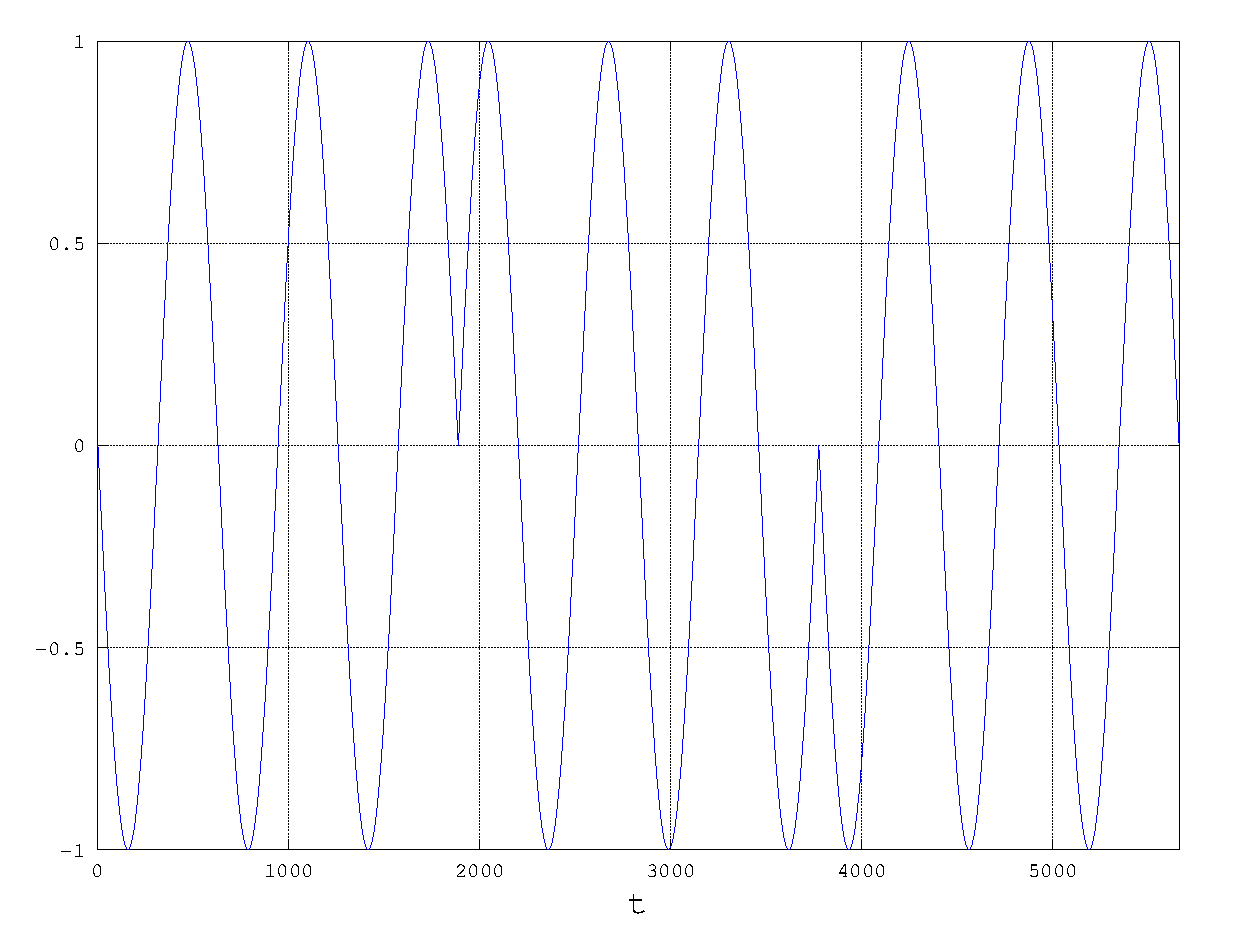
\includegraphics[width=1\linewidth]{bpsk.eps}}
\caption{Сигнал с модуляцией ДФМ}
\label{pic:sec1_bpsk}
\end{figure}
На рисунке \ref{pic:sec1_bpsk} представлена несущая, модулированная ДФМ.

Демодуляция производится повторной модуляцией принятого сигнала с синхронизированной копией ПСП ${C_k(t) - \tau}$, где
${\tau}$ - оценка фазы ПСП. При идеальной синхронизации сигнала, представленного вырежением \ref{eq:gps_signal},
c локальной копией ПСП, после демодуляции получаем:
\begin{center}
\begin{eqnarray}
	\label{eq:gps_signal_modulated}
	s_k(t) & = & \sqrt{2A}(C^2_k(t)D_k(t))\cos(\omega_{c}t) \nonumber \\
	& = &\sqrt{2A}D_k(t)\cos(\omega_{c}t)
\end{eqnarray}
\end{center}
Таким образом, на выходе демодулятора получается сигнал с суженным спектром. Следует отметить, что правильная оценка ${\tau}$
является одной из основных задач при детектировании сигнала, так как ПСП имеет пик корреляции только в пределах центрального пика
АКФ \cite{gold-ieee}  - синхронизация с точностью до одного чипа. При неверной оценке фазы ПСП в результате демодуляции спектр
ШПС не будет сужен, что приведет к ошибочным результатам на следующих этапах решения: вычислении уровня шума и принятии решения
о наличии или отсутсивии сигнала заданного спутника в анализируемых данных.

\begin{figure}[H]
\center\scalebox{0.5}{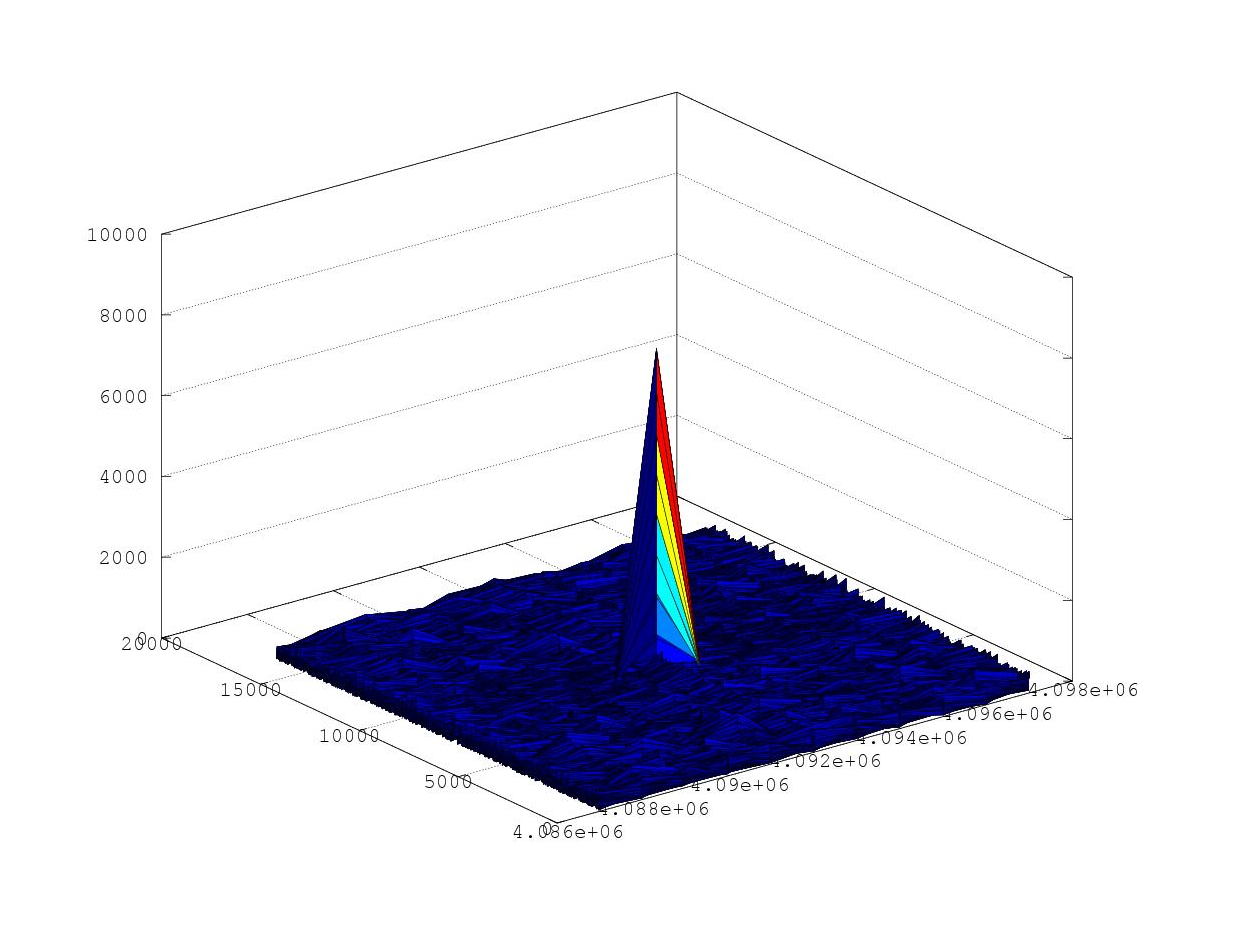
\includegraphics[width=1\linewidth]{corr_peak.eps}}
\caption{График ФН}
\label{pic:corr_peak}
\end{figure}

Задача поиска сигнала сводится к устранению неопределенности по двум параметрам: центральной частоте его спектра
и фазе ПСП. На рисунке \ref{pic:ambiguity_region} представлена область неопределенности. Можно заметить, что сечение
области неопределенности плоскостью ${f}$ представляет собой КФ сигнала. Поиск сигнала соответствует поиску и
оценке основного пика КФ.

\begin{figure}[H]
\center\scalebox{0.5}{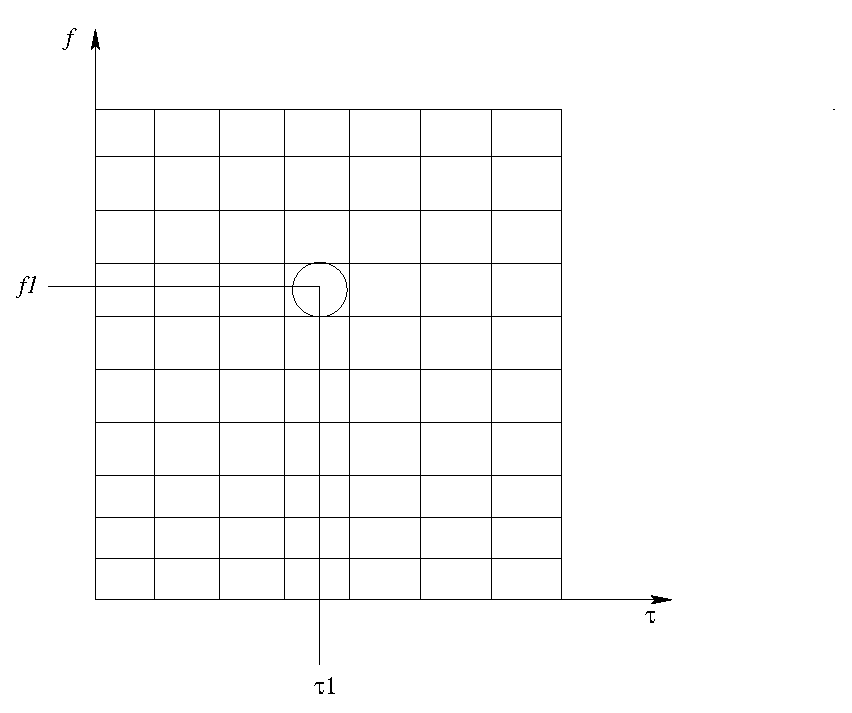
\includegraphics[width=1\linewidth]{ambiguity_region.eps}}
\caption{Область неопределенности}
\label{pic:ambiguity_region}
\end{figure}

\subsubsection{Модели помех}
\label{l:noise_model}
Обнаружение и распознавание помех всегда происходит в условиях действия помех и, решая задачу оптимизации приема,
необходимо иметь в виду определенные модели помех. Основноной помехой является флюктуационная с нормальным
распределением мнгновенных значений и широким равномерным энергетическим спектром. Такие помехи характеризуются
плотностью мощности ${N_n}$ на входе схемы оптимальной обработки \cite{pestryakov-book}.

Вторым видом помех, оказывающих
большое влияние на прием сигналов, являются помехи, связанные с рассеянным или многолучевым распространением
радиосигналов. Многолучевое распространение радиоволн, можно рассматривать или как фактор, обуславливающий
наличие дополнительных помех в виде сигналов, аналогичных тому, который рассматривается как основной, но с другой
задержкой, или как фактор изменающий статистические характеристики параметров принимаемого сигнала,
обуславливая случайность амплитуды \cite{pestryakov-book}.

Третьим видом помех, характерных для систем связи, использующих ШПС, являются помехи от шумоподобных сигналов,
принадлежащих другим адресам (каналам). Этои помехи определяются тем, что при использовании ШПС для разделения
сигналов по форме (кодовое разделение) сигналы, принадлежащие другим адресам, не являясь идеально ортогональными,
создают помехи. Сумма нескольких шумоподобных сигналов дает результирующий процесс, близкий к нормальному шуму,
поэтому помеху, создаваемую многими ШПС, во многих случаях можно рассматривать как нормальный шум с ограниченным
равномерным спектром и ограниченной мощностью \cite{pestryakov-book}.

Мощность помех подвергается значительным изменениям; это относится и к флюктуационным естественным помехам, так как
изменяются собственные шумы приемника, помехи, создаваемые атмосферой и космосом, усиление приемного устройства
и т.п. Следовательно, для основного вида помехи ее плотность мощности ${N_n}$ является случайной величиной.

В системе Navstar GPS можно выделить 6 источников помех \cite{parkinson_1996}:
\begin{itemize}
	\item {данные эфемерид - ошибки в позициях спутников;}
	\item {часы спутника - ошибки в переданных данных о времени;}
	\item {ионосфера - ошибки в коррекции псевдодальностей обусловленных ионосферными эффектами;}
	\item {тропосфера - ошибки в коррекции псевдодальностей обусловленных обусловленных тропосферными эффектами;}
	\item {Многолучевость - эффект отраженных сигналов принятых антенной;}
	\item {приемник - ошибки в измерениях обусловленные термальным шумом, точностью ПО и т.д.}
\end{itemize}

Так как данные виды помех влияют только на точность определения координат, мы можем рассматривать упрощенную модель
канала, где все данные виды помех не рассматриваются отдельно. Более углубленные модели канала можно найти в
источниках: упощенная модель канала с сигналом на промежуточной частоте \cite{lei_dong_phd}, модель многолучевого
распротранения \cite{hannah_phd}, а так же \cite{burns_model, corbell_model, crs_model, brown_model}.
 
\subsection{Классическая постановка задачи}
\label{sec1_FIXME}

Из литературы по теории атвоматических систем, например \cite{pugachev} (глава 10.1), известна классическая постановка
задачи задачи теории оптимальных систем. "На практике часто приходится решать задачу проектирования системы, когда
требуется определить характеристики системы таким образом, чтобы она имела наибольшую точность при данных условиях.
Систему обеспечивающую наибольшую возможную точность с какой-нибудь определенной точки зрения среди всех систем
заданного класса, обычно называют оптимальной" \cite{pugachev}.

В одной из постановок данной задачи \cite{pugachev} (глава 10.1), система считается полностью неизвестной
и требуется определить ее оператор так, чтобы она была оптимальной с точки зрения принятого критерия качества. Эта
задача сводится к определению с наибольшей возможной точностью некоторых параметров, от которых зависит принимаемый
сигнал. Но при этом важно учитывать не только точность, но и другие файторы, так как проектируемая система должна
удовлетворять многим, часто протеворечивым требованиям. В виду приведенных факторов, обычно представляет собой
ряд компромисных решений, удовлетворяющих всем предъявляемым к системе требованиям.

\subsection{Статистические криетрии оптимальности}
Точность автоматической системы обычно характеризуется математическим ожиданием и дисперсией ее ошибки.
Математическое ожидание представляет собой систематическую ошибку системы в данных условиях, а дисперсия
характеризует уровень случайных ошибок \cite{pugachev} (глава 10.2). Так как в различных условиях работы
системы, которые встречаются случайно систематическая ошибка тоже является случайной, за критерий качества
системы при ее проектировании обычно принимают второй начальный момент ошибки - математическое ожидание
квадрата ошибки ошибки:
\begin{center}
\begin{equation}
	\label{eq:stat_err_prob}
	\eta = M[E^2(t)]
\end{equation}
\end{center}
Положительный квадратный корень из этой величины называют средней квадратичной ошибкой системы. Таким образом,
оптимальной системой обычно считают такую систему, которая ммеет минимальную среднюю квадратичную ошибку.

Критерий минимума средней квадратичной ошибки является простейшим с математической точки зрения и обычно приводит
к наиболее простым методам определения оптимальных систем. Однако далеко не во всех задачах он может служить мерой
качества системы. Поэтому нельзя ограничиваться методами нахождения оптимальных систем по критерию минимума средней
квадратичной ошибки.

В случаях, когда необходимо проектировать следящую систему, приходится учитывать возможность срыва слежения,
который заключается в том что система перестает работать, если ее ошибка превосходит по абсолютной величине некоторый
уровень. При проектировании таких систем целосообразно принять за критерий качества вероятность срыва слежения. При
этом оптимальной считается такая система, которая обеспечивает минимум вероятности срыва слежения. Если срыв слежения
происходит в случае, когда абсолютная величинаошибки превосходит уровень $a$, то критерий минимума вероятности ошибки
слежения можно представить \cite{pugachev} (глава 10.2):
\begin{center}
\begin{equation}
	\label{eq:prob_lost_signal}
	p = P(E(t) > a) = min
\end{equation}
\end{center}

Так же применяют метод вычисления среднего риска $R$, как математического ожидания
от функции потерь $l(Y, Y_T)$ (подробнее \cite{pugachev} глава 10.2):
\begin{center}
\begin{equation}
	\label{eq:prob_lost_func}
	R = M(l(Y, Y_T))
\end{equation}
\end{center}

\subsection{Введение обозначений}
В предыдущих разделах было рассмотрено подробно структура ШПС, применяемого в системе Navstar GPS. В данном разделе
будут введены обозначения для дальнейшего использования в данной работе.

Обозначим модель входного СНС для ${K}$ - спутников как:
\begin{center}
\begin{equation}
	\label{eq:gps_model_1}
	s_k(t) = \sum_{k=1}^{K}{A_{k}C_{k}(t-\tau_k)D_{k}(t-\tau_k))\cos(\omega_{c}t + \phi_k)}
\end{equation}
\end{center}
где: ${A}$ - мощность сигнала, ${C_k}$ - ПСП для ${k}$ - сигнала, ${D}$ - данные, а ${\omega_{c}t}$ - частота несущей сигнала.

\subsection{Оптимальный приемник сигнала сигнала}

Оптимальный приемник сигнала состоит из оптимальной обработки сигнала и операции сравнения (или принятия решения). Стоит отметить,
что схема оптимальной обработки сигнала не зависит от операции принятия решения, так как как операция принятия решения зависит от
априорных сведений (например $A$, $\phi_k$ в \ref{eq:gps_model_1}). Для реализации оптимального приемника при неизвестных априорных
сведений схема оптимальной обработки сигнала останется старой, а вот правила выбора порога будут другими \cite{pestryakov-book}.

При обнаружении некоторе время производится наблюдение за смесью, в результате чего формируется реализация $s(t)$ (индекс $k$
опущен, так как для простоты изложения рассматривается один сигнал после операции умножения сигнала на ПСП источника $k$) или
выборка $s_{1}s_{2}...$ Эта реализация может принадлежать одной помехе или смеси сигнала и помехи. Для получения аналитического
выражения для оптимального алгоритма (правила) обработки смеси при принятии решений (гипотез) о наличии сигнала или его отсутствии,
нужно вероятностно описать протекание за длительное время смеси при наличии в ней сигнала и помехи или действия только помехи. Для
этого нужно выписать функции распределения смеси, содержащей только флюктуационную помеху в виде нормального гауссового шума:

\begin{center}
\begin{eqnarray}
	\label{eq:just_noise}
	w(x_{1}x_{2}.../n) & = & \frac{1}{(2\pi\sigma_{n}^{2})^{k_n/2}}\exp[-\frac{1}{2\sigma_{n}^{2}}\sum_{j=1}^{k_n}x_{j}^2] = \\
			& = & \frac{1}{(2\pi\sigma_{n}^{2})^{k_n/2}}\exp[-\frac{1}{N_n}\int_{0}^{T_n}x^2(t)] \nonumber
\end{eqnarray}
\end{center}
где $k_n=T_n/\tau_{kn}=2T_nf_{n}$ - объем выборки; ${T_n}$ - время наблюдения; ${f_{n}}$ - высшая частота в спектре помехи;
${N_n}$ - плотность мощности помехи; ${\sigma_{n}^{2}}$ - дисперсия помехи; ${t_{kn}}$ - интервао корреляции помехи.

Смесь сигнала и помехи можно записать как:
\begin{center}
\begin{equation}
	\label{eq:signal_and_noise}
	x(t) = s(t, \beta_1, \beta_2, ...) + n(t)
\end{equation}
\end{center}
Смесь также является случайным процессм. Условная многомерная функция распределения значений смеси при условии, что параметры
сигнала ${\beta_1, \beta_2, ...}$ имеют определенное значение, равна:
\begin{center}
\begin{eqnarray}
	\label{eq:signal_and_noise2}
	w(x_{1}x_{2}...x_{k}/\beta_1 \beta_2 ..., n) & = & \\
	& = & \frac{1}{(2\pi\sigma_{n}^{2})^{k_n/2}}\exp[-\frac{1}{N_n}\int_{0}^{T_n}[x(t) - s(t, \beta_1, \beta_2, ...)]^2 dt] \nonumber
\end{eqnarray}
\end{center}



Приведенное доказательство заимствовано из \cite{pugachev} (глава 13.4)

\newpage
		% базовая постановка вопроса

% detection 
\subsection{Алгоритмы детектирования сигнала}

\subsubsection{Коррелятор}

\paragraph{Последовательный коррелятор}
\label{sec1_serial}
Данный алгоритм в некоторых источниках так же называется согласованным фильтром. В \cite{sklyar} рассмотрены нюансы этих двух понятий.
В данной работе мы будем использовать понятие последовательный коррелятор. Работа коррелятора описывается математической операцией
корреляции \ref{eq:serial_corr}. Сигнал коррелируется с локальной копией и на выходе коррелятора получается значение, отражающее
степень совпадения сигналов. Не трудно представить, что сигнал с хорошими корреляционными свойствами должен обладать высоким значением
корреляции когда сигналы синхронизированы и минимальным значением в любом другом случае (фаза ПСП-кода не выровнена, отсутствие сигнала).

\begin{equation}
	\label{eq:serial_corr}
	y(n)=\sum\limits_{m=0}^{N-1}{x(m)h(n+m)}
\end{equation}
где: ${x(m)}$ - принятый сигнал, а ${h(n)}$ не импульсная характеристика системы, а локальная копия сигнала.

\paragraph{Параллельный коррелятор}
\label{sec1_fft}
Вычисление циклической свертки через дискретное преобразование Фурье (ДПФ) является достаточно популярным методом
в программных приемниках, так как позволяет существенно 
уменьшить количество элементарных операций при вычислении. Но как показано в \cite{tsui, oppenheim} можно достаточно просто
перейти от свертки к циклической корреляции. Так как этот метод является самым популярным в программных приемниках, рассмотрим его
подробнее.

Обозначим импульсный отклик системы через $h(n)$, а через ${x(n)}$ - входной сигнал. Тогда выходной сигнал в дискретном
временной домене можно записать как:

\begin{equation}
	\label{eq:fft_conv}
	y(n)=\sum\limits_{m=0}^{N-1}{x(m)h(n-m)}
\end{equation}

Стоит отметить, что в \ref{eq:fft_conv} сдвиг во времени является циклическим, поскольку дискретные операции являются циклическими.
Возьмем ДПФ от \ref{eq:fft_conv}

\begin{center}
\begin{eqnarray}
	\label{eq:fft_conv_fft}
	Y(k) & = & \sum\limits_{n=0}^{N-1}\sum\limits_{m=0}^{N-1}{x(m)h(n-m)e^{(-j2\pi{kn})/N}}=\nonumber \\
	& = & \sum\limits_{m=0}^{N-1}{x(m)}[\sum\limits_{n=0}^{N-1}h(n-m)e^{(-j2\pi{(n-m)}k)/N}]e^{(-j2\pi{m}k)/N}=\\
	& = & H(k)\sum\limits_{m=0}^{N-1}e^{(-j2\pi{m}k)/N} = X(k)H(k)\nonumber 
\end{eqnarray}
\end{center}


Из уравнения \ref{eq:fft_conv_fft} легко видеть, что это не линейная свертка. В линейной свертке для $N$ входного
сигнала и свертки результатом будет $2N-1$ точек. А в уравнении выше, результатом является всего $N$ точек.
Это является результатом циклической природы ДПФ.

Алгоритм детектирования не использует свертку, он использует корреляцию, которая отличается от свертки. Корреляция
между $x(n)$ и $h(n)$ может быть записана как:

\begin{equation}
	\label{eq:fft_corr}
	y(n) = \sum\limits_{m=0}^{N-1}{x(m)h(n+m)}
\end{equation}
Единственным отличаем между \ref{eq:fft_conv} и \ref{eq:fft_corr} является знак перед $m$ в ${h(n+m)}$.
В случае детектирования сигнала $h(n)$ является локальной копией сигнала, а не импульсной характеристикой.
Произведем ДПФ над $z(n)$:

\begin{center}
\begin{eqnarray}
	\label{eq:fft_corr_fft}
	Z(k) & = & \sum\limits_{n=0}^{N-1}\sum\limits_{m=0}^{N-1}{x(m)h(n+m)e^{(-j2\pi{kn})/N}}=\nonumber \\
	& = & \sum\limits_{m=0}^{N-1}{x(m)}[\sum\limits_{n=0}^{N-1}h(n+m)e^{(-j2\pi{(n+m)}k)/N}]e^{(j2\pi{m}k)/N}=\\
	& = & H(k)\sum\limits_{m=0}^{N-1}e^{(j2\pi{m}k)/N} = X(k)H^{-1}(k)\nonumber 
\end{eqnarray}
\end{center}
где ${X^{-1}(k)}$ - обратное ДПФ. Уравнение \ref{eq:fft_corr_fft} можно записать как:

\begin{equation}
	\label{eq:fft_corr_fft_rev}
	Y(k) = \sum\limits_{n=0}^{N-1}\sum\limits_{m=0}^{N-1}{x(n+m)h(m)e^{(-j2\pi{kn})/N}}=X^{-1}(k)H(k)
\end{equation}

Если сигнал $x(n)$ реальный, то $x(n) = x^*(n)$, где * - операция комплексного сопряжения. Используя данное соотношение,
значение $Z(k)$ может быть записано:
\begin{equation}
	\label{eq:fft_magnitude}
	|Z(k)|=|H^*(k)X(k)|=|H(k)X(k)^*|
\end{equation}
Данное соотношение может быть использовано для нахождения значения циклической корреляции между входным сигналом и 
локальной копией.

\paragraph{ФАПЧ}
Программные приемники системы Navstar GPS рассмотрены в \cite{tsui, akos-book}.
После стадии детектирования сигнала, оценка частоты для заданного источника поступает в модуль уточнения частоты.
Уточненная частота и фаза ПСП поступают в ФАПЧ.

Одним из параметров системы ФАПЧ является шумовая полоса.
Этот параметр определяет количество теплового шума попадающего в систему ФАПЧ. Широкая шумовая полоса позволяет системе ФАПЧ быстро войти в синхронизм,
но также ведет к существенному ухудшению характеристик системы ФАПЧ за счет возрастания уровня теплового шума.

Область допутимой расстройки частоты, в пределах которой обеспечивается захват, при ${\zeta>0.3}$ определяется как \cite{spilker-book}:
\begin{center}
\begin{equation}
	\label{eq:corr_pll_band}
	\Delta \omega_m = 2 \omega_n (\zeta + 0.6)
\end{equation}
\end{center}
где ${\omega_n}$ - собственная частота системы ФАПЧ, ${\zeta}$ - коэффициент демпфирования,

В \cite{tsui, spilker-book} предложено брать ${\zeta=0.707}$, тогда ${\Delta \omega_m = 2.614 \omega_n}$.
Собственная частота модуля фазовой автоподстройки частоты вычисляется по формуле:
\begin{center}
\begin{equation}
	\label{eq:corr_pll_freq}
	\omega_n = \frac{8 \zeta B_L}{4 \zeta^2 + 1} 
\end{equation}
\end{center}
где ${B_L}$ - шумовая полоса.

Традиционный подход детектирования сигнала предусматривает корреляцию входного сигнала и набора локальных копий сигнала шагом 1 кГц.
Для стационарного приемника Navstar GPS диапазон смещения частоты обусловленный допплеровским эффектом \cite{tsui} может находится в диапазоне ${\pm 5}$ кГц.
Таким образом, для получения оценки с точностью 1 кГц необходимо провести поиск в 11 ячейках. В каждой ячейке нам необходимо ${N}$-комплексных умножений.
Для наземных приемников типовое значение  ${B_L=20}$ Гц \cite{tsui, akos-book}. Область синхронизации из выражения \ref{eq:corr_pll_band} и  \ref{eq:corr_pll_freq}.
${\Delta \omega_m \approx 100}$ Гц. Таким образом необходима стадия уточнения частоты.

Схема традиционного приемника изображена на рисунке \ref{pic:corr_scheme}.
\begin{figure}[H]
	\center\scalebox{1}{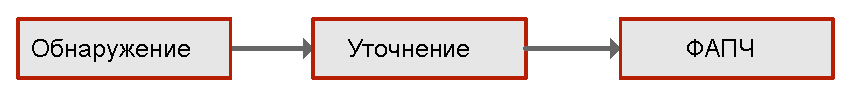
\includegraphics[width=1\linewidth]{corr_scheme.eps}}
	\caption{Схема традиционного приемника}
	\label{pic:corr_scheme}
\end{figure}

Количество комплексных умножений, требуемых для оценки частоты одного источника параллельным коррелятором: ${OP_{FFT} = 12NlogN + 11N}$

Алгоритм уточнения частоты описан в \cite{tsui}. Следует отметить, что данный алгоритм основан на усреднении фазы и требует дополнительной оперативной памяти
(ОЗУ) приемника для хранения 5 миллисекунд данных при обработке одного источника. Оперативная память потребляет значительное количество энергии,
поэтому снижение количества необходимой ОЗУ является важной задачей при разработке портативных приемников.
Так же обработка 5 мс данных повышает встретить переход бита внутри данных – это ведет к дополнительным сложностям при реализации программных приемников сигнала Navstar GPS.

Количество умножений, требуемых для уточнения частоты одного источника: ${OP_{FINE} = }$

\newpage
 		%
\subsubsection{Детектирование слабого сигнала с помощью осциллятора Дуффинга}
\label{ssec:duffing}

Теория колебаний и волн возникла примерно в 18 веке. Ее началом принято считать труды Лагранжа, опубликованные в 1788 г. Введя обобщенные
координаты и импульсы, Лагранж, отошел от традиционной механики и записал динамические уравнения, которые могут быть отнесены к системам
любой природы. Подробную историю возникновения теории колебаний и волн можно найти во введении к \cite{landa_book}. 
Введем некоторые используемые в работе термины.

\emph{Аттрактором} называется множество точек в фазовом пространстве, к которому стремятся со
временем все соседние фазовые траектории из некоторой области, называемой областью притяжения \cite{landa_book}.

\emph{Динамической системой} называют такую систему, движение которой задается набором правил. Для динамической системы можно ввести
понятие \emph{состояние}, определяемого набором величин, называемых \emph{динамическими переменными}.

\emph{Фазовое пространство} - пространство динамических переменных, полностью определяющих состояние системы.

\emph{Ляпуновский показатель} - 
характеризует степень расходимости близких фазовых траекторий, и число положительных ляпуновских показателей, характеризующее число направлений
неустойчивости. Максимальный ляпуновский показатель:
\begin{center}
\begin{equation}
	\label{eq:exp_lyapunova_1}
	\lambda = \lim_{\substack{t \to \infty\\d \to 0}}\ln \frac{d(t)}{d(0)},
\end{equation}
\end{center}
где ${d(t)}$ - расстояние между двумя близкими фазовыми траекториями. Непосредственный рассчет показателей по данной формуле является
затруднительным для систем с экспененциальной неустойчивостью траектории. В \cite{landa_book} рассмотрен более простой способ:
\begin{center}
\begin{equation}
	\label{eq:exp_lyapunova_2}
	\lambda = \frac{1}{m}\sum \limits_{i=1}^m \lambda_i = \frac{1}{m\tau}\ln\prod \limits_{i=1}^md_i,
\end{equation}
\end{center}
где локальный ляпуновский показатель ${\lambda_i}=(1/ \tau)\ln d_i$, ${d_i}$ - отношение расстояние между траекториями в конце ${i}$ - го
шага к начальному расстоянию.

Динамическая система описываемая уравнением \ref{eq:oscillator_basic} на двумерной фазовой плоскости называется - осциллятором (система
описываемая на двумерном фазовом цилиндре - ротаторе в данной работе не рассматривается)\cite{chaos_neimark_landa}.
\begin{center}
\begin{equation}
	\label{eq:oscillator_basic}
	x'' + 2\delta(x, x') + Q(x) = 0
\end{equation}
\end{center}

Частным случаем уравнения \ref{eq:oscillator_basic} является уравнение Дуффинга, которое описывает явление нелинейного резонанса:
\begin{center}
\begin{equation}
	\label{eq:oscillator_duffing}
	x'' + 2\delta{x'} + ax +bx^3 = F\cos{\nu{t}}
\end{equation}
\end{center}

Детектирование сигналов с расширенным спекторм (в частности сигналов системы Navstar GPS) с помощью осциллятора Дуффинга
достаточно новое направление в исследованиях по данной тематике. В частности
\cite{chaos_chen, chaos_cambridge, chaos_huang, chaos_song}. Так же является интересной более ранняя статья не рассматривающая GPS
\cite{chaos_wang}.

Осциллятор Дуффинга с периодическим внешним воздействием может быть описан уравнением \ref{eq:duffing}:
\begin{center}
\begin{equation}
	\label{eq:duffing}
	mx'' + cx' + k_{1}x + k_{2}x^3 = F_{0}\cos(\omega{t})
\end{equation}
\end{center}

где
$m$- масса,
$c$ - коэффициент диссипации,
$x$ - состояние осциллятора,
$k_1$ и $k_2$ - линейный и нелинейный коэффициенты соответственно.
$F_{0}\cos(\omega{t})$ - внешнее воздействие.

Подробно уравнение \ref{eq:duffing} рассмотрено в \cite{chaos_neimark_landa} (Глава 9 параграф 3). Но
для использования осциллятора Дуффинга для детектирования сигналов системы GPS былa предложена
усовершенствованная форма данного осциллятора \cite{chaos_song, chaos_chen}:

\begin{center}
\begin{equation}
	\label{eq:duffing_gps}
	x'' +cx' - x^3 + x^5 = \gamma\cos(\omega{t}) + (\gamma_{x}\cos(\omega_{x}) + n(t))
\end{equation}
\end{center}

Перепишем динамическую систему \ref{eq:duffing_gps} в виде:
\begin{center}
\begin{eqnarray}
	\label{eq:duffing_gps_2}
	y(t) & = & x'(t) \\
	y'(t) & = & -cx' + x^3 - x^5 + \gamma\cos(\omega{t}) + (\gamma_{x}\cos(\omega_{x}) + n(t))
\end{eqnarray}
\end{center}

Пример фазового портрета при ${\omega=\omega_{x}}$ изображен на рисунке \ref{pic:duffing_sync},
фазовый портрет хаоса расположен на рисунках \ref{pic:duffing_chaos1}, \ref{pic:duffing_chaos2}
\begin{figure}[H]
	\center\scalebox{0.5}{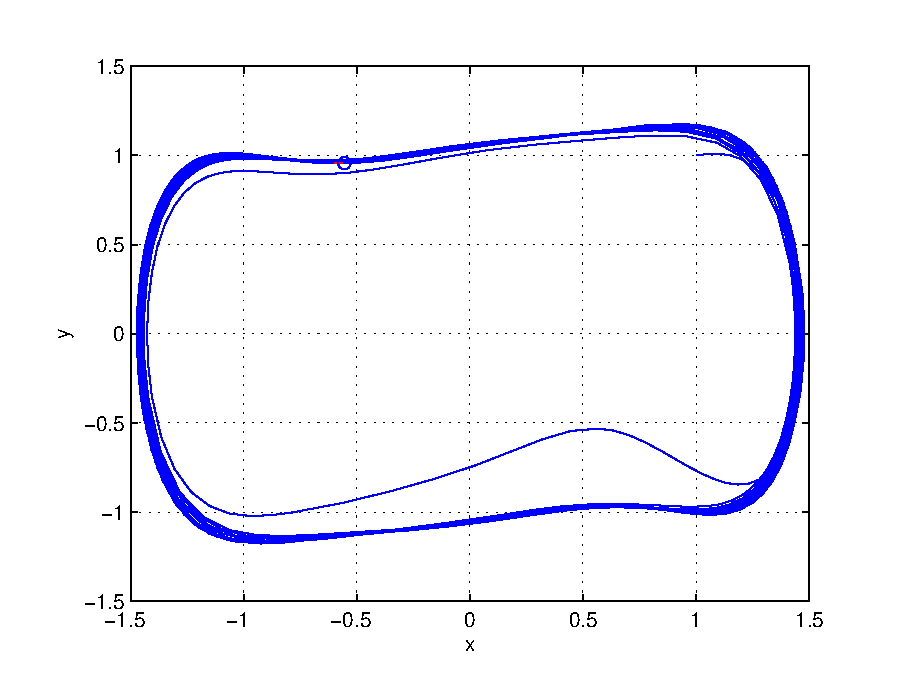
\includegraphics[width=1\linewidth]{duffing_sync.eps}}
	\caption{Фазовый портрет при ${\omega =\omega_{x}}$}
	\label{pic:duffing_sync}
\end{figure}

\begin{figure}[H]
	\center\scalebox{0.5}{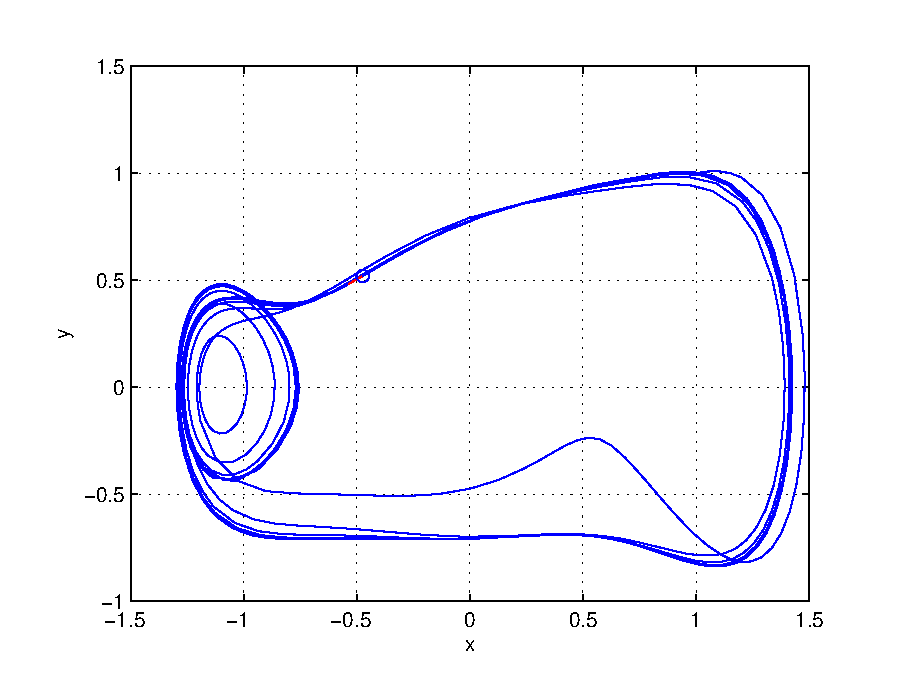
\includegraphics[width=1\linewidth]{duffing_chaos1.eps}}
	\caption{Фазовый портрет при ${\omega < \omega_{x}}$}
	\label{pic:duffing_chaos1}
\end{figure}

\begin{figure}[H]
	\center\scalebox{0.5}{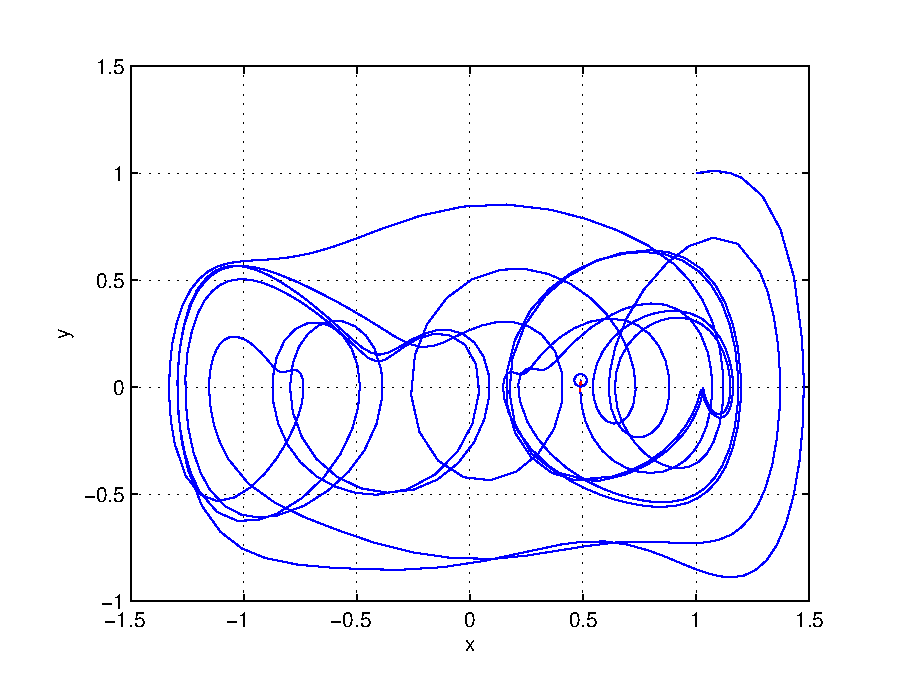
\includegraphics[width=1\linewidth]{duffing_chaos2.eps}}
	\caption{Фазовый портрет при ${\omega > \omega_{x}}$}
	\label{pic:duffing_chaos2}
\end{figure}

В качестве параметров уравнения применялись $c = 0.5$, $\gamma=\gamma_{x}=0.36$, ${\omega=1}$

Часто для вычисления характеристик хаотической динамики применяется показатель Ляпунова.
Он показывает в каком состоянии находится система. Если система находится
в стабильном состоянии линии фазовой траектории будут близко прилегать одна к другой, в противном
случае система находится в состоянии хаоса. Детектор с применением показателя ляпунова
представлен на рисунке \ref{pic:chaos_lyapunov}.

\begin{figure}[H]
	\center\scalebox{0.7}{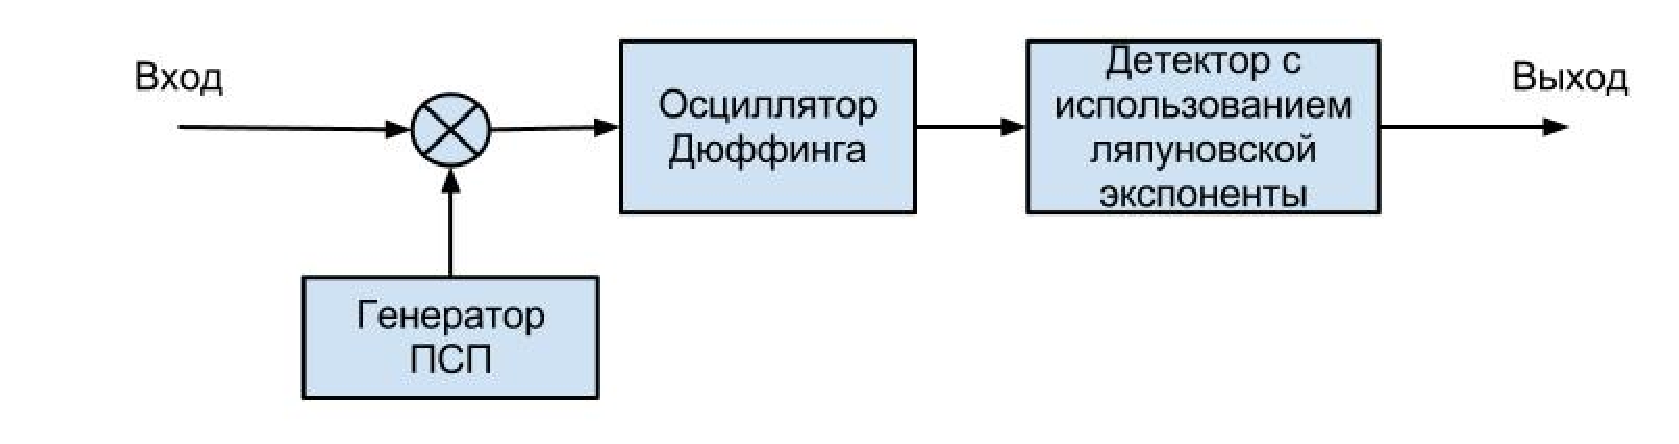
\includegraphics[width=1\linewidth]{Chaos_detector_Lyapunov.eps}}
	\caption{Схема детектора основанного на показателе ляпунова для осциллятора Дуффинга}
	\label{pic:chaos_lyapunov}
\end{figure}

В статье \cite{chaos_chen} предложен усовершенствованный метод, базирующийся на вычислении дисперсии
фазовой траектории. Действительно, на рисунках \ref{pic:duffing_sync}, \ref{pic:duffing_chaos1},
\ref{pic:duffing_chaos2} видно - когда система находится в хаотическом состоянии значение
дисперсии по координате ${x}$, чем соответствующее значение в состоянии $\omega = \omega_{x}$.
На основе этого была предложена усовершенствованная схема детектора сигнала
\ref{pic:chaos_energy_detector}

\begin{figure}[H]
	\center\scalebox{0.7}{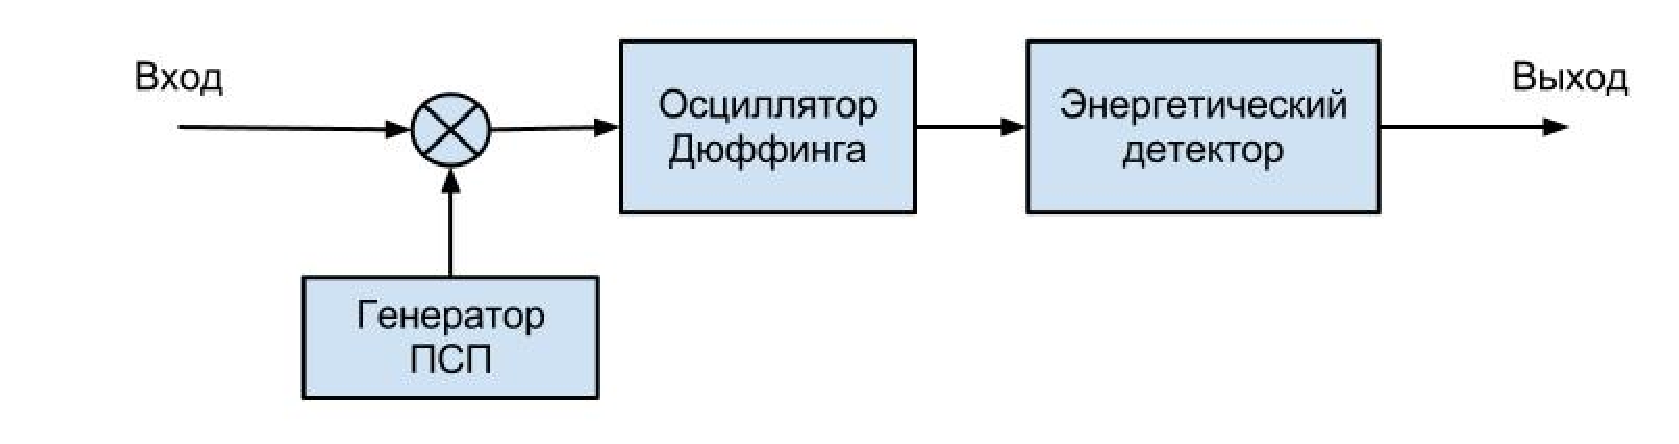
\includegraphics[width=1\linewidth]{chaos_detector.eps}}
	\caption{Схема энергетического детектора для осциллятора Дуффинга}
	\label{pic:chaos_energy_detector}
\end{figure}

\newpage
		%
\subsubsection{Алгоритм детектирования с применением статистик высоких порядков}
\label{sbs:sec1_hos}

Математический аппарат статистик высоких порядков (СВП или HOS - Higher-order statistics)
для исследования не причинных, причинных и нестабильных
(систем с не минимальной фазой) и не-Гауссовых сигналов впервые был предложен в \cite{hos_petropulu} в 1993 году.
Этот метод позволяет не только подавлять цветной Гауссов шум, но так же в некоторых случаях подавлять
цветной не-Гауссов шум.

В работе \cite{hos_zhao} был предложен метод детектирования ШПС с использованием СВП.

\newpage
		% Higher-order statistics

%optimization
\subsection{Методы оптимизации алгоритмов}
\subsubsection{Коррелятор}

\paragraph{Параллельный коррелятор}
\label{sec1_fft}
Вычисление циклической свертки через дискретное преобразование Фурье (ДПФ) является достаточно популярным методом
в программных приемниках, так как позволяет существенно 
уменьшить количество элементарных операций при вычислении. Но как показано в \cite{tsui, oppenheim} можно достаточно просто
перейти от свертки к циклической корреляции. Так как этот метод является самым популярным в программных приемниках, рассмотрим его
подробнее.

Обозначим импульсный отклик системы через $h(n)$, а через ${x(n)}$ - входной сигнал. Тогда выходной сигнал в дискретном
временной домене можно записать как:

\begin{equation}
	\label{eq:fft_conv}
	y(n)=\sum\limits_{m=0}^{N-1}{x(m)h(n-m)}
\end{equation}

Стоит отметить, что в \ref{eq:fft_conv} сдвиг во времени является циклическим, поскольку дискретные операции являются циклическими.
Возьмем ДПФ от \ref{eq:fft_conv}

\begin{center}
\begin{eqnarray}
	\label{eq:fft_conv_fft}
	Y(k) & = & \sum\limits_{n=0}^{N-1}\sum\limits_{m=0}^{N-1}{x(m)h(n-m)e^{(-j2\pi{kn})/N}}=\nonumber \\
	& = & \sum\limits_{m=0}^{N-1}{x(m)}[\sum\limits_{n=0}^{N-1}h(n-m)e^{(-j2\pi{(n-m)}k)/N}]e^{(-j2\pi{m}k)/N}=\\
	& = & H(k)\sum\limits_{m=0}^{N-1}e^{(-j2\pi{m}k)/N} = X(k)H(k)\nonumber 
\end{eqnarray}
\end{center}


Из уравнения \ref{eq:fft_conv_fft} легко видеть, что это не линейная свертка. В линейной свертке для $N$ входного
сигнала и свертки результатом будет $2N-1$ точек. А в уравнении выше, результатом является всего $N$ точек.
Это является результатом циклической природы ДПФ.

Алгоритм детектирования не использует свертку, он использует корреляцию, которая отличается от свертки. Корреляция
между $x(n)$ и $h(n)$ может быть записана как:

\begin{equation}
	\label{eq:fft_corr}
	y(n) = \sum\limits_{m=0}^{N-1}{x(m)h(n+m)}
\end{equation}
Единственным отличаем между \ref{eq:fft_conv} и \ref{eq:fft_corr} является знак перед $m$ в ${h(n+m)}$.
В случае детектирования сигнала $h(n)$ является локальной копией сигнала, а не импульсной характеристикой.
Произведем ДПФ над $z(n)$:

\begin{center}
\begin{eqnarray}
	\label{eq:fft_corr_fft}
	Z(k) & = & \sum\limits_{n=0}^{N-1}\sum\limits_{m=0}^{N-1}{x(m)h(n+m)e^{(-j2\pi{kn})/N}}=\nonumber \\
	& = & \sum\limits_{m=0}^{N-1}{x(m)}[\sum\limits_{n=0}^{N-1}h(n+m)e^{(-j2\pi{(n+m)}k)/N}]e^{(j2\pi{m}k)/N}=\\
	& = & H(k)\sum\limits_{m=0}^{N-1}e^{(j2\pi{m}k)/N} = X(k)H^{-1}(k)\nonumber 
\end{eqnarray}
\end{center}
где ${X^{-1}(k)}$ - обратное ДПФ. Уравнение \ref{eq:fft_corr_fft} можно записать как:

\begin{equation}
	\label{eq:fft_corr_fft_rev}
	Y(k) = \sum\limits_{n=0}^{N-1}\sum\limits_{m=0}^{N-1}{x(n+m)h(m)e^{(-j2\pi{kn})/N}}=X^{-1}(k)H(k)
\end{equation}

Если сигнал $x(n)$ реальный, то $x(n) = x^*(n)$, где * - операция комплексного сопряжения. Используя данное соотнешение,
значение $Z(k)$ может быть записано:
\begin{equation}
	\label{eq:fft_magnitude}
	|Z(k)|=|H^*(k)X(k)|=|H(k)X(k)^*|
\end{equation}
Данное соотношение может быть использовано для нахождения значения циклической корреляции между входным сигналом и 
локальной копией.

\newpage
	%
\section{Алгоритм delay and multiply approach}

Алгоритм был предаставлен в книге и статье американского ученого Дж.
Цуя \cite{lin_dma, tsui}

Пусть входной комплексный сигнал описывается формулой:

\begin{center}
\begin{equation}
	s(t)=A(t)e^{j2{\pi}f_{0}t}\label{eq:dma_lo_signal}
\end{equation}
\end{center}

где $A(t)$ - амплитуда, а$f_{0}$- частота сигнала.

Если входящий комплексный сигнал имеет задержку $\tau$, то данный
сигнал будет описываться формулой: 

\begin{center}
\begin{equation}
	\label{eq:dma_signal}
	s(t-\tau)=A(t-\tau)e^{j2{\pi}f_{0}(t-\tau)}
\end{equation}
\end{center}

Получим новый сигнал путем умножения \ref{eq:dma_lo_signal} и \ref{eq:dma_signal}:

\begin{center}
\begin{eqnarray}
s_{n}(t) & = & s(t)s(t-\tau)^{*}=\nonumber \\
 & = & A(t)A(t-\tau)e^{j2\pi f_{0}t}e^{j2\pi f(t-\tau)}=\label{eq:dma}\\
 & = & A(t)A(t-\tau)e^{j2\pi f_{0}\tau}\nonumber 
\end{eqnarray}

\par\end{center}

Из формулы \ref{eq:dma} видно, что полученный сигнал не зависит от
задержки $\tau$. Остается найти фазу C/A кода. Референсный сигнал
$A(t)A(t-\tau)$ используется для корреляции с новым кодом, который
получен по формуле (3) - умножением принятого сигнала и его задержанной
копии. Когда фаза C/A кода найдена, поиск сводится к одномерному поиску
частоты. Данный метод позволяет уменьшить количество вычислений, путем
сведения задачи поиска в двух измерения: по фазе кода и частоте; к
задаче поиска только по частоте. Этот метод позволяет существенно
сэкономить вычислительные ресурсы при обнаружении сигнала заданного
спутника, но, вместе с тем, операция умножения повышает шум в процессе.

Анализ шума алгоритма DMA 

\begin{center}
\begin{eqnarray}
	s_{n}(t) & = & (s(t)+n_{1}(t))(s(t-\tau)+n_{2}(t))^{*}=\nonumber \\
	 & = & A(t)A(t-\tau)e^{j2{\pi}f_{0}{\tau}}+\nonumber \\
	 & + & A(t)e^{j2{\pi}f_{0}t}n_{2}(t)+\label{eq:dma_noise}\\
	 & + & A(t-\tau)e^{j2{\pi}f_{0}(t-\tau)}n_{1}(t)+\nonumber \\
	 & + & n(t)^{2}\nonumber 
\end{eqnarray}
\end{center}

где $A(t)A(t-\tau)e^{j2{\pi}f_{0}{\tau}}$ - новый C/A код, а $n(t)^{2}+A(t)e^{j2{\pi}f_{0}t}n_{2}(t)+A(t-\tau)e^{j2{\pi}f_{0}(t-\tau)}n_{1}(t)$-
шумовая компонента.

Поскольку корреляция производится с \textquotedbl{}новым\textquotedbl{}
кодом $A(t)A(t-\tau)$, компонента $A(t)e^{j2{\pi}f_{0}t}n_{2}(t)+A(t-\tau)e^{j2{\pi}f_{0}(t-\tau)}n_{1}(t)$
будет являеться шумом,$n(t)^{2}$ - квадрат АБГШ.

\newpage
		%
\subsection{Алгоритм нахождения пика AКФ}

Данный алгоритм представлен в работах \cite{2max_ieee, 2max_article}. Его оригинальное название
\textquotedblleft{Peak-finding algorithm}\textquotedblright,
в данной работе введем перевод -
\textquotedblleft{Алгоритм нахождения пика}\textquotedblright (АНП). 

Алгоритм был разработан для улучшения рабочих характеристик традиционных алгоритмов рассмотренных в
\ref{sec1_serial} и \ref{sec1_fft}. Предложенный алгоритм можно разбить на несколько шагов:
\begin{itemize}
\item[Шаг 1] Подсчитать АКФ, используя метод предложенный в \ref{sec1_fft}.
\item[Шаг 2] Найти главный пик АКФ, найти второй пик АКФ, найти среднее значение АКФ.
\item[Шаг 3] Нормализовать полученные значения относительно главного пика АКФ.
\item[Шаг 4] Если (максимум АКФ - среднее) > ${V_{th1}}$ и (максимум АКФ - 
	второй максимум АКФ) > ${V_{th2}}$, тогда полученный главный пик АКФ соответсвует
	искомой фазе кода и частоте.
\end{itemize}

В статье авторов \cite{2max_ieee} предложенны следующие значения для порогов:
${V_{th1}} = 0.3$(Дб) и  ${V_{th2}} = 0.15$(Дб). Так же авторы предлагают итерационную процедуру для нахождения
фазы ПСП и частоты смещения допплера:
\begin{itemize}
\item[Шаг 1] Начать вычисление с 1мс.
\item[Шаг 2] Получить результаты АНП.
\item[Шаг 3] Если фаза ПСП и частота не могут быть найдены, увеличить время интегрироавния сигнала.
	Использовать следующие значения для интегрирования: 1мс -> 10мс -> 50мс -> 100мс -> 200мс ->
	500мс -> 1000мс
\end{itemize}

%\begin{center}
%\begin{equation}
%	\label{eq:dma_signal}
%	SNR(dB) = 10\log{\frac{max[d(n)] - mean[d(n)]}{std[d(n)]}}
%\end{equation}
%\end{center}

\newpage
		%

% noise
\subsection{Постановка задачи оценки шума}
\label{sssec:sec1_noise_est}

Задача оценки отношения сигнал-шума (ОСШ) является одной из ключевых при детектировании сигналов.
ОСШ используется в задаче определения порога детектирования рисунок \ref{pic:sec1_gnss_system}.
При превышении порога спутник считается задетектированным, если же порог
не превышен, считается, что сигнал данного спутника в данных не присутствует.

Пусть для данной задачи входной сигнал описывается соотношением \cite{presti_ieee}:
\begin{center}
\begin{equation}
	\label{eq:noise_est_signal}
	s_C[t]=\sqrt{P_d}D[n] + \sqrt{P_n}\eta[n]
\end{equation}
\end{center}
где $D[n]$ - биты навигационного сообщения, $\eta[n]=\eta_{Re} + j\eta_{Im}$ - комплексный шум,
$P_d$ - мощность сигнала, а $P_n$ - мощность шума (обе величины берутся на выходе коррелятора).
Стоит отметить, что $D[n]=a_{n}e^{j\theta_n}$, где $a_n=\pm{1}$ для сигналов с двоичной модуляцией, а
$\theta_n$ - остаточная фазовая ошибка от контура ФАПЧ слежения за частотой.
Тогда ОСШ для $s_C[t]$ можно представить как:
\begin{center}
\begin{equation}
	\label{eq:noise_est_snr}
	\lambda_C=\frac{P_d}{P_n}
\end{equation}
\end{center}
От выражения \ref{eq:noise_est_snr} можно перейти к соотношению количества шума на герц $C/N_0$:
\begin{center}
\begin{equation}
	\label{eq:noise_est_cn}
	\lambda_C=\frac{C}{N_{0}B_{eqn}}\Rightarrow\frac{C}{N_0}=\lambda_{C}B_{eqn}
\end{equation}
\end{center}
В \cite{presti_ieee} показано, что $B_{eqn}$ можно выразить:
\begin{center}
\begin{equation}
	\label{eq:noise_est_beqn}
	B_{eqn}=\frac{1}{T_{int}}
\end{equation}
\end{center}
где ${T_{int}}$ - время интегрирования.

%%%%%%%%%%%%%%%%%%%%%%%%%%%%%%%%%%%%%%%%%%%%%%%%%%%%%%
\subsubsection{Алгоритм оценки ОСШ
\textquotedblleftдействительный сигнал - комплексный шум\textquotedblright}
\label{sssec:rscn}

В иностранной литературе он называется "Real Signal - Complex Noise (RSCN)". Введем перевод
"Действительный сигнал - комлексный шум (ДСКШ)".
Данный алгоритм рассмотрен в статьях \cite{badke_rscn, presti_insidegnss, presti_ieee}.

Если рассматривать идеально синхронизированный сигнал, тогда в синфазном контуре будет
находится сигнал и АБГШ, в то время как в квадратурном плече будет находится только шум,
независимый и одинаково распределенный с шумом в синфазном контуре. Данный факт может
быть использован для оценки ОСШ в программном приемнике:
\begin{center}
\begin{equation}
	\label{eq:rscn_noise_power}
	\hat{P_n} = \frac{2}{N}\sum^N_{v=1}|r_{C,Im}[v]|^2
\end{equation}
\end{center}

\begin{center}
\begin{equation}
	\label{eq:rscn_total_power}
	\hat{P}_{tot} = \frac{1}{N}\sum^N_{v=1}|r_{C}[v]|^2
\end{equation}
\end{center}

\begin{center}
\begin{equation}
	\label{eq:rscn_data_power}
	\hat{P_d} = \hat{P}_{tot} - \hat{P_n}
\end{equation}
\end{center}

\begin{center}
\begin{equation}
	\label{eq:rscn_snr}
	\hat{\lambda_C} = \frac{\hat{P_d}}{\hat{P_n}} = \frac{\hat{P}_{tot} - \hat{P_n}}{\hat{P_n}} 
\end{equation}
\end{center}

Очевидно, что данный метод является чувствительным к сдвигу фазы, который приводит к переходу энергии
в квадратурный контур. Любой остаточный сдвиг фазы ведет к возрастанию энергии шума в квадратурном
контуре (это видно из \ref{eq:rscn_noise_power}).

%%%%%%%%%%%%%%%%%%%%%%%%%%%%%%%%%%%%%%%%%%%%%%%%%%%%%%
\subsubsection{Алгоритм Signal-to-Noise Variance}
\label{sssec:snv}

Данный алгоритм был представлен в \cite{snr_pauluzzi, snr_li}. Квадратичный ОСШ оценщик, основан на 1
и 2 моменте семплов сигнала:

\begin{center}
\begin{equation}
	%\label{eq:rscn_data_power}
	\hat{P_{d}} = (\frac{1}{N} \sum \limits_{v=1}^N \left| r_{C,Re}[v] \right|)^2
\end{equation}
\end{center}

\begin{center}
\begin{equation}
	%\label{eq:rscn_data_power}
	\hat P_{tot} = \frac{1}{N} \sum \limits_{v=1}^{N} \left|r_C[v] \right| ^2
\end{equation}
\end{center}

\begin{center}
\begin{equation}
	%\label{eq:rscn_snr}
	\hat{\lambda_C} = \frac{\hat P_d}{\hat P_{tot} - \hat P_d}
\end{equation}
\end{center}

%%%%%%%%%%%%%%%%%%%%%%%%%%%%%%%%%%%%%%%%%%%%%%%%%%%%%%
\subsubsection{Алгоритм Beaulieu}
\label{sssec:beaulieu}

Данный алгоритм был представлен в статье \cite{snr_beaulieu}.

\begin{center}
\begin{equation}
	%\label{eq:rscn_data_power}
	\hat{P_{n,v}} = (\left| r_{C,Re}[v] \right| - \left| r_{C,Re}[v-1] \right|)^2
\end{equation}
\end{center}

\begin{center}
\begin{equation}
	%\label{eq:rscn_data_power}
	\hat{P_{d,v}} = \frac{1}{2}(r_{C,Re}[v]^2 + r_{C,Re}[v-1]^2)
\end{equation}
\end{center}

\begin{center}
\begin{equation}
	%\label{eq:rscn_snr}
	\hat{\lambda_C} = [ \frac{1}{N} \sum \limits_{v=1}^{N} \frac{\hat P_{n,v}}{\hat P_{d,v}} ]^-1
\end{equation}
\end{center}

%%%%%%%%%%%%%%%%%%%%%%%%%%%%%%%%%%%%%%%%%%%%%%%%%%%%%%
\subsubsection{Алгоритм основанный на методе моментов}
\label{sssec:mm}
Данный алгоритм был представлен в \cite{snr_pauluzzi}. Он использует 2 и 4 статистические моменты для раздельной оценки
мощности сигнала и шума.
\begin{center}
\begin{equation}
	%\label{eq:rscn_data_power}
	\hat M_2 = \frac{1}{N} \sum \limits_{v=1}^{N} \left|r_C[v] \right| ^2
\end{equation}
\end{center}

\begin{center}
\begin{equation}
	%\label{eq:rscn_data_power}
	\hat M_2 = \frac{1}{N} \sum \limits_{v=1}^{N} \left|r_C[v] \right| ^4
\end{equation}
\end{center}

\begin{center}
\begin{equation}
	%\label{eq:rscn_data_power}
	\hat P_d = \sqrt{2 \hat M^2_2 - \hat M_4} 
\end{equation}
\end{center}

\begin{center}
\begin{equation}
	%\label{eq:rscn_data_power}
	\hat P_n = \hat M_2 - \hat P_d
\end{equation}
\end{center}

\begin{center}
\begin{equation}
	%\label{eq:rscn_snr}
	\hat{\lambda_C} = \frac{\hat P_d}{\hat P_n}
\end{equation}
\end{center}

%%%%%%%%%%%%%%%%%%%%%%%%%%%%%%%%%%%%%%%%%%%%%%%%%%%%%%
\subsubsection{Алгоритм Narrowband-Wideband Power Ratio}
\label{sssec:nwpr}

Данный алгоритм был представлен в \cite{parkinson_1996}, а так же в нескольких других книгах по СНРС GPS. Особенностью данного алгоритма
является то, что это единственный алгоритм производящий оценку ${C/N_0}$, а не ОСШ, который может быть преобразован ${C/N_0}$.

\begin{center}
\begin{equation}
	%\label{eq:rscn_data_power}
	WBP_k = \sum \limits_{m=1}^{M} \left|r_C[kM+m] \right| ^2, k=0,1,...(\frac{N}{M}-1)
\end{equation}
\end{center}

\begin{center}
\begin{equation}
	%\label{eq:rscn_data_power}
	NBP_k = (\sum \limits_{m=1}^{M} \left|r_{C,Re}[kM+m] \right| )^2 + (\sum \limits_{m=1}^{M} \left|r_{C,Im}[kM+m] \right| )^2
\end{equation}
\end{center}

\begin{center}
\begin{equation}
	%\label{eq:rscn_data_power}
	\hat \mu_{NP} = \frac{M}{N} \sum \limits_{k=0}^{N/M-1} \frac{NBP_k}{WBP_k}
\end{equation}
\end{center}

\begin{center}
\begin{equation}
	%\label{eq:rscn_data_power}
	\gamma = \frac{C}{N_0} = \frac{1}{T_{int}} \frac{\hat \mu_{NP} - 1}{M - \hat \mu_{NP}}
\end{equation}
\end{center}

%%%%%%%%%%%%%%%%%%%%%%%%%%%%%%%%%%%%%%%%%%%%%%%%%%%%%%
\subsubsection{Выводы}
Алгоритмы, приведенные в разделах \ref{sssec:rscn}, \ref{sssec:snv}, \ref{sssec:beaulieu}, \ref{sssec:mm}, \ref{sssec:nwpr}
подробно рассмотрены в \cite{presti_ieee}. Получены их оценки по количеству операций, а так же
исследованы свойства аппроксимации данных функций.

Следует отметить, что данные алгоритмы работают только с синхронизированным сигналом.

\newpage
		% постановка вопроса оценки шума
% так зверски сделаны кавычки
\subsection{Алгоритм оценки ОСШ
\textquotedblleftдействительный сигнал - комплексный шум\textquotedblright}

В иностранной литературе он называется "Real Signal - Complex Noise (RSCN)". Введем перевод
"Действительный сигнал - комлексный шум (ДСКШ)".
Данный алгоритм рассмотрен в статьях \cite{badke_rscn, presti_insidegnss, presti_ieee}.

Если рассматривать идеально синхронизированный сигнал, тогда в синфазном контуре будет
находится сигнал и АБГШ, в то время как в квадратурном плече будет находится только шум,
независимый и одинаково распределенный с шумом в синфазном контуре. Данный факт может
быть использован для оценки ОСШ в программном приемнике:
\begin{center}
\begin{equation}
	\label{eq:rscn_noise_power}
	\hat{P_n} = \frac{2}{N}\sum^N_{v=1}|r_{C,Im}[v]|^2
\end{equation}
\end{center}

\begin{center}
\begin{equation}
	\label{eq:rscn_total_power}
	\hat{P}_{tot} = \frac{1}{N}\sum^N_{v=1}|r_{C}[v]|^2
\end{equation}
\end{center}

\begin{center}
\begin{equation}
	\label{eq:rscn_data_power}
	\hat{P_d} = \hat{P}_{tot} - \hat{P_n}
\end{equation}
\end{center}

\begin{center}
\begin{equation}
	\label{eq:rscn_snr}
	\hat{\lambda_C} = \frac{\hat{P_d}}{\hat{P_n}} = \frac{\hat{P}_{tot} - \hat{P_n}}{\hat{P_n}} 
\end{equation}
\end{center}

Очевидно, что данный метод является чувствительным к сдвигу фазы, который приводит к переходу энергии
в квадратурный контур. Любой остаточный сдвиг фазы ведет к возрастанию энергии шума в квадратурном
контуре (это видно из \ref{eq:rscn_noise_power}).

\newpage
		% rscn - алгоритм

\section{Глава 2}
\section{Использование осциллятора Дуффинга для детектирования сигнала}
Теория колебаний и волн возникла примерно в 18 веке. Ее началом принято считать труды Лагранжа, опубликованные в 1788 г. Введя обобщенные
координаты и импульсы, Лагранж, отошел от традиционной механики и записал динамические уравнения, которые могут быть отнесены к системам
любой природы. Подробную историю возникновения теории колебаний и волн можно найти во введении к \cite{landa_book}. 
Введем некоторые используемые в работе термины.

\emph{Аттрактором} называется множество точек в фазовом пространстве, к которому стремятся со
временем все соседние фазовые траектории из некоторой области, называемой областью притяжения \cite{landa_book}.

\emph{Ляпуновский показатель} - 
характеризует степень расходимости близких фазовых траекторий, и число положительных ляпуновских показателей, характеризующее число направлений
неустойчивости. Максимальный ляпуновский показатель:
\begin{center}
\begin{equation}
	\label{eq:exp_lyapunova_1}
	\lambda = \lim \limits_{t \to \infty, d \to 0} = \ln \frac{d(t)}{d(0)},
\end{equation}
\end{center}
где ${d(t)}$ - расстояние между двумя близкими фазовыми траекториями. Непосредственный рассчет показателей по данной формуле является
затруднительным для систем с экспененциальной неустойчивостью траектории. В \cite{landa_book} рассмотрен более простой способ:
\begin{center}
\begin{equation}
	\label{eq:exp_lyapunova_2}
	\lambda = \frac{1}{m}\sum \limits_{i=1}^m \lambda_i = \frac{1}{m\tau}\ln\prod \limits_{i=1}^md_i,
\end{equation}
\end{center}
где локальный ляпуновский показатель ${\lambda_i}=(1/ \tau)\ln d_i$, ${d_i}$ - отношение расстояние между траекториями в конце ${i}$ - го
шага к начальному расстоянию.

Динамическая система описываемая уравнением \ref{eq:oscillator_basic} на двумерной фазовой плоскости называется - осциллятором (система
описываемая на двумерном фазовом цилиндре - ротаторе в данной работе не рассматривается)\cite{chaos_neimark_landa}.
\begin{center}
\begin{equation}
	\label{eq:oscillator_basic}
	x'' + 2\delta(x, x') + Q(x) = 0
\end{equation}
\end{center}

Частным случаем уравнения \ref{eq:oscillator_basic} является уравнение Дуффинга, которое описывает явление нелинейного резонанса:
\begin{center}
\begin{equation}
	\label{eq:oscillator_duffing}
	x'' + 2\delta{x'} + ax +bx^3 = F\cos{\nu{t}}
\end{equation}
\end{center}

\newpage

\subsection{Спектральный анализ}
Спектральный анализ - это один из методов обработки сигналов, который позволяет охарактеризовать частотный состав измеряемого сигнала.
Методы статистики играют важную роль в спектральном анализе, поскольку сигналы, как правило, имеют шумовой или случайный характер. Если бы
основные статистические характеристики сигнала были известны точно или же их можно было бы без ошибк определить на конечном интервале этого
сигнала, то спектральный анализ представлял бы собой отрасль точной науки. В действительноти по одному-единственному отрезку сигнала можно
получить только некоторую оценку его спектра. Практика спектрального анализа после 1880-х гг. постепенно стала превращаеться в некое ремесло
достаточно субъективного характера, которое на ряду с использованием научного подхода требовало также определенного уровня эмпирического
искусства \cite{marpl_book}.

Математические основы современных методов спектрального оценивания берут свое начало в XVII веке в работах И. Ньютона, который установил, что
солнечный свет, прошедший через стеклянную призму, разлагается на многоцветную полосу. В которой каждому цвету соответствует своя длинна волны.

\subsubsection{Применение нормального уравнения Юла-Уолкера}
В 1927 г. Дж. Юл предложил существенно новый метод спектрального анализа. Для отыскаяния одной-двух переодичностей в исследуемых данных Юл
прибег к моделированию временного ряда, основанному на линейном регрессионном анализе. Юла интересовала главным образом более высокая точность
определения основной периодичности в ряде чисел солнечных пятен и отыскания в нем дополнительных периодичностей \cite{marpl_book}.
Используя простое тригонометрическое тождество:
\begin{center}
\begin{equation}
	\label{eq:yule_trigonometric}
	\sin(kx)=2\cos(x)\sin([k-1]x)-sin([k-2]x)
\end{equation}
\end{center}
Используя подстановки и обобщая формулу (весь ход обобщения описан в \cite{marpl_book}) можно получить:
\begin{center}
\begin{equation}
	\label{eq:yule_raznost}
	u(k) = b(1)u(k-1) + b(2)u(k-2) + \epsilon (k)
\end{equation}
\end{center}
Здесь ${u(k) = \sin (2\pi fkT)}$ - гармоническая составляющая, ${T}$ - интервал отсчетов, ${f}$ - частота гармоник, а
${b(1)}$ и ${b(2)}$ принимают произвольные значения. Как легко увидеть, уравнение \ref{eq:yule_raznost} представляет собой АР уравнение, и это был
первый случай когда АР по методу наименьших квадратор применялась для целей спектроанализа. Решением уравнения \ref{eq:yule_raznost}
является затухающая синусойда.

АР модель предсказания отсчета может быть описана как взвешенная сумма ${P}$ предыдущих отсчетов сигнала:
\begin{center}
\begin{equation}
	\label{eq:lpc_forecast}
	\hat{x(m)} = \sum \limits_{i=1}^P a_k x(m-k),
\end{equation}
\end{center}
Где ${\hat{x(m)}}$ - оценка ${x(m)}$ в момент времени ${m}$, а ${a_k}$ - коэффициенты АР модели.

Оценка ошибки ${e(m)}$ может быть представлена как:
\begin{center}
\begin{equation}
	\label{eq:lpc_error}
	e(m) = x(m) - \hat{x(m)} = x(m) - \sum \limits_{i=1}^P a_k x(m-k),
\end{equation}
\end{center}

Из уравнения \ref{eq:lpc_error} смоделированный сигнал может быть представлен следующим рекурсивным соотношением:
\begin{center}
\begin{equation}
	\label{eq:lpc_signal}
	x(m) = \sum \limits_{i=1}^P a_k x(m-k) + e(m)
\end{equation}
\end{center}

Уравнения \ref{eq:lpc_error} представляет собой цифровой фильтр.
После ${z}$ - преобразования уравнение \ref{eq:lpc_signal} может быть записана как \cite{saeed_book}:
\begin{center}
\begin{eqnarray}
	\label{eq:lpc_z}
		H(z)	& = & \frac{X(z)}{U(z)} = \frac{G}{1 - \sum \limits_{k=1}^P a_kz^{-k}} =  \nonumber \\
			& = & G\frac{1}{\prod \limits_{k=1}^N (1-r_kz^{-1})} \frac{1}{\prod \limits_{k=1}^M (1-2r_k \cos \phi_k z^{-1} + r_k^2z^{-2})}
\end{eqnarray}
\end{center}

В уравнении \ref{eq:lpc_z} ${M}$ - пары комплексных полюсов, ${N}$ - действиьедбные полюсы с ${P=N+2M}$,
${r_k}$ и ${\phi_k}$ - радиус и угол ${k}$ - го полюса соответственно. Частотный ответ такой системы 
может быть представлен \cite{saeed_book}:
\begin{center}
\begin{eqnarray}
	\label{eq:lpc_freq_resp}
		H(f)	& = & = \frac{G}{1 - \sum \limits_{k=1}^P a_k e^{-j2 \pi kf}} =  \nonumber \\
			& = & G\frac{1}{\prod \limits_{k=1}^N (1-r_k e^{-j2 \pi f)}} \frac{1}{\prod \limits_{k=1}^M (1-2r_k \cos \phi_k e^{-j2 \pi f} + r_k^2 e^{-j4 \pi f})}
\end{eqnarray}
\end{center}

\paragraph{Вычисление коэффициентов АР модели}
Наилучшие оценки коэффициентов ${a_k}$ могут быть получены минимизацией среднеквадратичной ошибки уравнения\cite{saeed_book}
\ref{eq:lpc_error}:
\begin{center}
\begin{eqnarray}
	\label{eq:lpc_rms}
		E[e^2(m)]	& = & E[(x(m) - \sum \limits_{i=1}^P a_k x(m-k))^2] =\nonumber \\
				& = & E[x^2(m)] - \nonumber \\
				& &  - 2\sum \limits_{i=1}^P a_k E[x(m-k)x(m)] + \nonumber \\
				& &  + \sum \limits_{i=1}^P a_k \sum \limits_{j=1}^P a_j E[x(m-k)x(m-j)] = \nonumber \\
				& = & r_{xx}(0) - 2{\bf r}^T_{xx}{bf a} + {\bf a}^T {\bf R_{xx}a}
\end{eqnarray}
\end{center}
Где ${{\bf R_{xx}} = E[{\bf xx}^T]}$ - это автокорреляционная матрица входного вектора ${{\bf x}^T=[x(m-1),x(m-2),...,x(m-P)]}$,
${{\bf r}_{xx}=E[x(m){\bf x}]}$ - автокорреляционный вектор, а ${a^T=[a_1,a_2,...,a_P]}$ -  вектор коэффициентов предсказателя.
Минимизация среднеквадратичной ошибки из уравнения \ref{eq:lpc_rms} может быть записана как:
\begin{center}
\begin{equation}
	\label{eq:lpc_rms2}
	{\bf a=R^{-1}_{xx}r_{xx}}
\end{equation}
\end{center}

Можно использовать альтернативную запись.
Для сигнала длинной в ${N}$ семплов можно записать ${N}$ - уравнений:
\begin{center}
\begin{equation}
	\label{eq:lpc_rms3}
	{\bf e=x-Xa}
\end{equation}
\end{center}
Уравнение \ref{eq:lpc_rms3} можно переписать в виде:
\begin{center}
\begin{equation}
	\label{eq:lpc_rms4}
	{\bf eу^T = xx^T - 2x^T Xa + a^T X^T Xa}
\end{equation}
\end{center}

Взяв производную по вектору ${{\bf a}}$, можно получить параметры предсказателя:
\begin{center}
\begin{equation}
	\label{eq:lpc_rms5}
	\frac{\partial {\bf e^T e}}{\partial {\bf a}} = {\bf - 2x^T X + a^T X^T X} = 0
\end{equation}
\end{center}
Из \ref{eq:lpc_rms6}, коэффициенты для минимальной среднеквадратичной ошибки равны:
\begin{center}
\begin{equation}
	\label{eq:lpc_rms6}
	{\bf a= (X^T X)^{-1} (X^T x)}
\end{equation}
\end{center}

Из сравнения уравнений \ref{eq:lpc_rms2} и \ref{eq:lpc_rms6} видно, что в \ref{eq:lpc_rms2}
автокорреляционная матрица и вектор заменеы оценками:
\begin{center}
\begin{equation}
	\label{eq:lpc_rms7}
	\hat{r_{xx}}(m) = \frac{1}{N} \sum \limits_{k=0}^{N-1} x(k)x(k-m)
\end{equation}
\end{center}

Уравнения \ref{eq:lpc_rms2} и \ref{eq:lpc_rms7} могут быть эффиктивно решены с помощью регулярных
Тёплицевых структур корреляционной матрицы ${{\bf R_{xx}}}$. Эффективным алгоритмам над Тёплицевыми
матрицами посвещена книга \cite{bleyhut_book} (а это нужно????) Эффективным методом решения
данных соотношений является алгоритм Левинсона-Дарби.

АР метод оценивания СПМ часто используется для того, чтобы выявить в данных наличие синусоидальных
компонент. Мощность, соответствующую  таким компонентам в АР оценке СПМ, можно вычислить, интегрируя
площадь под кривой этой оценки. Однако это связано с большими вычислительными затратами, поэтому
гораздо более эффективным является использования в качестве показателя мощности синусоидальных
компонент высоты соответствующих им спектральных пиков \cite{marpl_book}.  

\newpage


\section{Глава 3}
\subsection{АР-модель случайного процесса. Оценка параметров АР-модели}

Модель линейного предсказателя может быть описана как взвешенная сумма ${P}$ предыдущих отсчетов сигнала:
\begin{center}
\begin{equation}
	\label{eq:lpc_forecast}
	\hat{x}(m) = \sum \limits_{k=1}^P a_k x(m-k),
\end{equation}
\end{center}
Где ${\hat{x}(m)}$ - оценка ${x(m)}$ в момент времени ${m}$, а ${a_k}$ - коэффициенты линейного предсказателя.

Ошибка предсказания ${e(m)}$ может быть представлена как разность между принятым семплом и его
предсказанным значением:
\begin{center}
\begin{equation}
	\label{eq:lpc_error}
	e(m) = x(m) - \hat{x}(m) = x(m) - \sum \limits_{k=1}^P a_k x(m-k),
\end{equation}
\end{center}

Из уравнения \ref{eq:lpc_error} смоделированный сигнал может быть представлен следующим рекурсивным соотношением:
\begin{center}
\begin{equation}
	\label{eq:lpc_signal}
	x(m) = \sum \limits_{k=1}^P a_k x(m-k) + e(m)
\end{equation}
\end{center}

Выражение \ref{eq:lpc_error} соответствует структуре выражения АР-модели при замене ошибки предсказания ${e(m)}$ на АБГШ.
Так же следует учесть, что входом линейного предсказателя является последовательность ${x(m)}$, а выходом ${e(m)}$.
В АР-модели выхдом является последовательность ${x(m)}$. Коэффициенты ${a_k}$ идентичны.
В виду этого существует тесная связь между фильтром линейного предсказания и АР-моделью \cite{marpl_book}.

Уравнение \ref{eq:lpc_error} представляет собой цифровой фильтр.
После ${z}$ - преобразования уравнение \ref{eq:lpc_signal} может быть записано как \cite{saeed_book}:
\begin{center}
\begin{eqnarray}
	\label{eq:lpc_z}
		H(z)	& = & \frac{X(z)}{U(z)} = \frac{G}{1 - \sum \limits_{k=1}^P a_kz^{-k}} =  \nonumber \\
			& = & G\frac{1}{\prod \limits_{k=1}^N (1-r_kz^{-1})} \frac{1}{\prod \limits_{k=1}^M (1-2r_k \cos \phi_k z^{-1} + r_k^2z^{-2})}
\end{eqnarray}
\end{center}

В уравнении \ref{eq:lpc_z} ${M}$ - пар комплексных полюсов, ${N}$ - действительные полюсы с ${P=N+2M}$,
${r_k}$ и ${\phi_k}$ - радиус и угол ${k}$ - го полюса соответственно. Частотный отклик такой системы 
может быть представлен \cite{saeed_book}:
\begin{center}
\begin{eqnarray}
	\label{eq:lpc_freq_resp}
		H(f)	& = & = \frac{G}{1 - \sum \limits_{k=1}^P a_k e^{-j2 \pi kf}} =  \nonumber \\
			& = & G\frac{1}{\prod \limits_{k=1}^N (1-r_k e^{-j2 \pi f)}} \frac{1}{\prod \limits_{k=1}^M (1-2r_k \cos \phi_k e^{-j2 \pi f} + r_k^2 e^{-j4 \pi f})}
\end{eqnarray}
\end{center}

На рисунке \ref{pic:lpc_poles} изображено отношение между полюсами и АЧХ рекурсивного фильтра. На частотах, соответствующих полюсам,
на графике АЧХ приаргумент комплексного полюса сутствуют частотные пики. Пары комплексных корней могут быть представлены через радиус ${r_k}$ и угол ${\phi_k}$
полюса:

\begin{center}
\begin{equation}
	\label{eq:lpc_poles}
	z_k = r_k e^{\pm j \phi_k}
\end{equation}
\end{center}

Резонансные частоты выражаются через комплексные полюса как:
\begin{center}
\begin{equation}
	\label{eq:lpc_poles_freq}
	F(\phi_k)=\frac{F_s}{2 \pi} \phi_k
\end{equation}
\end{center}
где ${F_s}$ - частота оцифровки, ${\phi_k}$ - аргумент комплексного полюса ${z_k}$ передаточной функции \ref{eq:lpc_z}.

\begin{figure}[H]
	\center\scalebox{1}{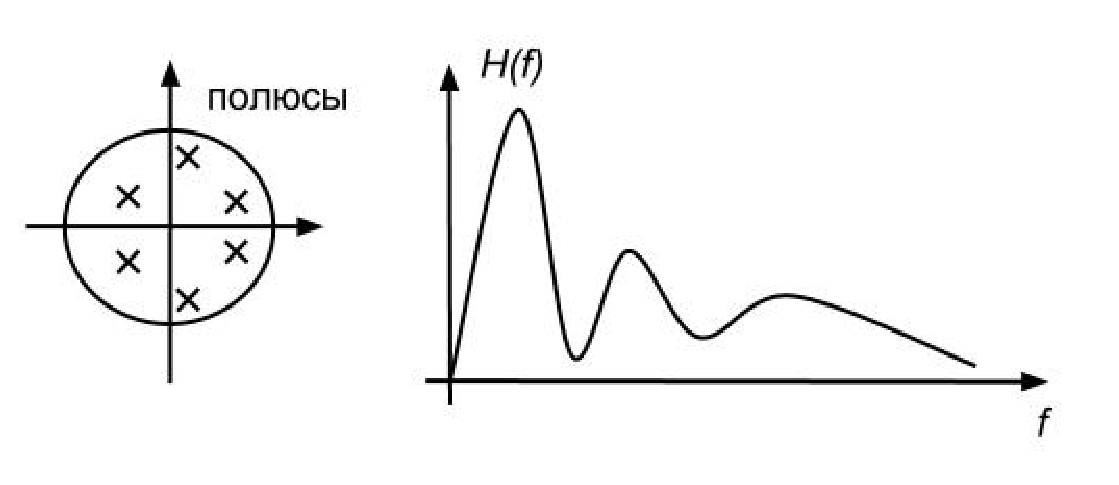
\includegraphics[width=1\linewidth]{lpc_poles.eps}}
	\caption{Полюса и АЧХ линейного предсказателя}
	\label{pic:lpc_poles}
\end{figure}

\paragraph{Вычисление коэффициентов АР модели}
Наилучшие оценки коэффициентов ${a_k}$ могут быть получены минимизацией среднеквадратичной ошибки уравнения\cite{saeed_book}
\ref{eq:lpc_error}:
\begin{center}
\begin{eqnarray}
	\label{eq:lpc_rms}
		E[e^2(m)]	& = & E[(x(m) - \sum \limits_{k=1}^P a_k x(m-k))^2] =\nonumber \\
				& = & E[x^2(m)] - \nonumber \\
				& &  - 2\sum \limits_{k=1}^P a_k E[x(m-k)x(m)] + \nonumber \\
				& &  + \sum \limits_{k=1}^P a_k \sum \limits_{j=1}^P a_j E[x(m-k)x(m-j)] = \nonumber \\
				& = & r_{xx}(0) - 2{\bf r}^T_{xx}{bf a} + {\bf a}^T {\bf R_{xx}a}
\end{eqnarray}
\end{center}
Где ${{\bf R_{xx}} = E[{\bf xx}^T]}$ - это автокорреляционная матрица входного вектора ${{\bf x}^T=[x(m-1),x(m-2),...,x(m-P)]}$,
${{\bf r}_{xx}=E[x(m){\bf x}]}$ - автокорреляционный вектор, а ${a^T=[a_1,a_2,...,a_P]}$ -  вектор коэффициентов предсказателя.
Минимизация среднеквадратичной ошибки из уравнения \ref{eq:lpc_rms} может быть записано как:
\begin{center}
\begin{equation}
	\label{eq:lpc_rms2}
	{\bf a=R^{-1}_{xx}r_{xx}}
\end{equation}
\end{center}

Можно использовать альтернативную запись.
Для сигнала длинной в ${N}$ семплов можно записать ${N}$ - уравнений:
\begin{center}
\begin{equation}
	\label{eq:lpc_rms3}
	{\bf e=x-Xa}
\end{equation}
\end{center}
Уравнение \ref{eq:lpc_rms3} можно переписать в виде:
\begin{center}
\begin{equation}
	\label{eq:lpc_rms4}
	{\bf eу^T = xx^T - 2x^T Xa + a^T X^T Xa}
\end{equation}
\end{center}

Взяв производную по вектору ${{\bf a}}$, можно получить параметры предсказателя:
\begin{center}
\begin{equation}
	\label{eq:lpc_rms5}
	\frac{\partial {\bf e^T e}}{\partial {\bf a}} = {\bf - 2x^T X + a^T X^T X} = 0
\end{equation}
\end{center}
Из \ref{eq:lpc_rms6}, коэффициенты для минимальной среднеквадратичной ошибки равны:
\begin{center}
\begin{equation}
	\label{eq:lpc_rms6}
	{\bf a= (X^T X)^{-1} (X^T x)}
\end{equation}
\end{center}

Из сравнения уравнений \ref{eq:lpc_rms2} и \ref{eq:lpc_rms6} видно, что в \ref{eq:lpc_rms2}
автокорреляционная матрица и вектор заменены оценками:
\begin{center}
\begin{equation}
	\label{eq:lpc_rms7}
	\hat{r}_{xx}(m) = \frac{1}{N} \sum \limits_{k=0}^{N-1} x(k)x(k-m)
\end{equation}
\end{center}

Уравнения \ref{eq:lpc_rms2} и \ref{eq:lpc_rms7} могут быть эффиктивно решены с помощью регулярных
Тёплицевых структур корреляционной матрицы ${{\bf R_{xx}}}$. Эффективным алгоритмам над Тёплицевыми
матрицами посвещена книга \cite{bleyhut_book} \textcolor{red}{<== А ЭТО НУЖНО????} Эффективным методом решения
данных соотношений является алгоритм Левинсона-Дарби.

АР метод оценивания СПМ часто используется для того, чтобы выявить в данных наличие синусоидальных
компонент. Мощность, соответствующую  таким компонентам в АР оценке СПМ, можно вычислить, интегрируя
площадь под кривой этой оценки. Однако это связано с большими вычислительными затратами, поэтому
гораздо более эффективным является использования в качестве показателя мощности синусоидальных
компонент высоты соответствующих им спектральных пиков \cite{marpl_book}.  

%%%%%%%%%%%%%%%%%%%%%%%%%%%%%%%%%%%%%%%%%%%%%%%%%%%%%%%%%%%%%%
\subsection{АР модель второго порядка. Оценка частоты основного тона на основе АР-модели}
АР-модель второого порядка применяется для определения частоты основого тона. Для поиска единственного
тона необходимо найти 2 полюса. Тогда выражение \ref{eq:lpc_rms2} может быть записано как:

\begin{center}
\begin{equation}
	\label{eq:lpc_gps_1}
	\left[ \begin{array}{c}
		\hat{a}_1 \\
		\hat{a}_2
	\end{array} \right]
	=
		\left[ \begin{array}{cc}
			r_{xx}(0) & r_{xx}(1) \\
			r_{xx}(1) & r_{xx}(0)
		\end{array} \right]^{-1}
		\left[ \begin{array}{c}
			r_{xx}(1) \\
			r_{xx}(2)
		\end{array} \right]
	= R_x^{-1}r_{xx1}
\end{equation}
\end{center}

Здесь ${\hat{a}_1, \hat{a}_2}$, - МНК оценки коэффициентов модели, ${r_{xx}(m)}$ - АКФ принимаемого сигнала.
Для оценки АКФ  можно использовать выражение:

\begin{center}
\begin{equation}
	\label{eq:lpc_rxx_estimation}
	\hat{r}_{xx}(m) = \frac{1}{N-1} \sum \limits_{k=0}^{N-1} x(k)x(k-m)
\end{equation}
\end{center}

Передаточная функция АР-модели второго порядка ${H(z)}$:
\begin{center}
\begin{equation}
	\label{eq:lpc_spectral_func}
	H(z) = \frac{1}{1 - a_1 z^{-1} - a_2 z^{-2}}
\end{equation}
\end{center}

Для определения резонансной частоты ${H(z)}$ можно воспользоваться формулой \ref{eq:lpc_poles_freq}.
Для принятия решения о наличии гармонического сигнала анализируют значение квадрата модуля частотной
характеристики АР-модели в точке резонанса:

\begin{center}
\begin{equation}
	\label{eq:lpc_power_cos}
	\left| H(z) \right|^2 = \frac{1}{\left| 1 - a_1 e^{-j \omega_0} - a_2 e^{-2 \omega_0} \right|^2}
\end{equation}
\end{center}

Если это значение превышает некоторый заранее выбранный порог, то принимается решение о наличии гармонического
сигнала с частотой  . 

%%%%%%%%%%%%%%%%%%%%%%%%%%%%%%%%%%%%%%%%%%%%%%%%%%%%%%%%%%%%%%
\subsection{Использование АР-модели для детектирования ШПС}

При работе с ПСП следует учитывать, что после демодуляции входного сигнала выровненной ПСП в сигнале восстанавливается 1 гармоническая
компонента, что дает возможность использовать АР-модель второго порядка.
Повторная модуляция сигнала с ПСП по любой фазе отличной от искомой не будет восстанавливать гармонический сигнал.
Спектр гармонического сигнала повторно модулированного ПСП с невыровненной фазой будет такой же, как у исходного сигнала – отображен
на рисунке \ref{pic:lpc_psd_1} штриховой пунктирной линией. И только повторная модуляция с выровненной фазой ПСП даст спектр
изображенный красной линией на рисунке \ref{pic:lpc_psd_1}.

На \ref{pic:lpc_basic1} входной сигнал повторно модулируется ПСП с известной фазой.

\begin{figure}[H]
	\center\scalebox{0.8}{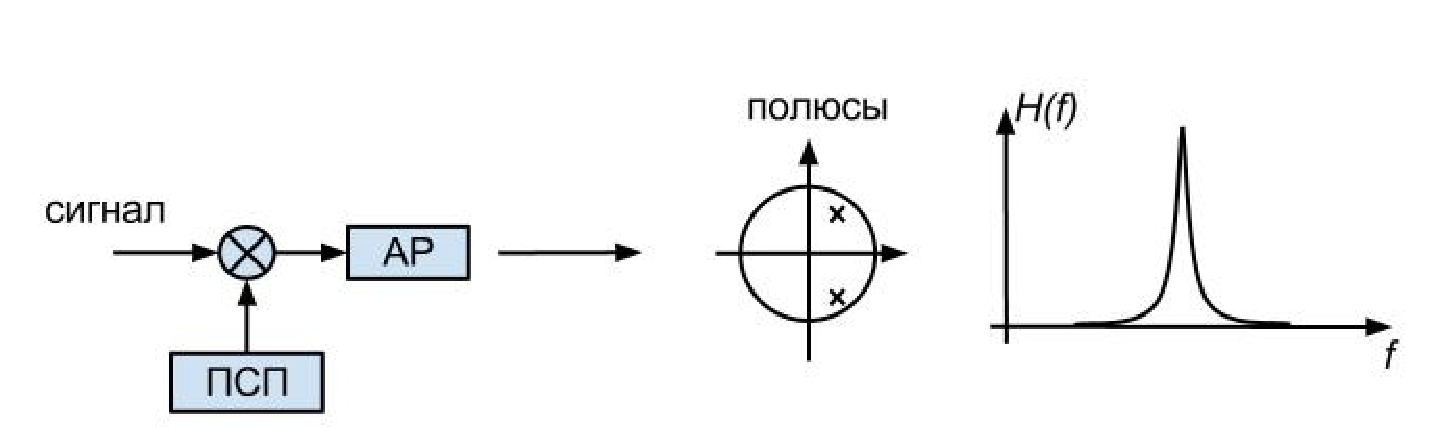
\includegraphics[width=1\linewidth]{lpc_basic.eps}}
	\caption{Общая схема применения АР-модели для детектирования ШПС сигнала}
	\label{pic:lpc_basic1}
\end{figure}

Выходом алгоритма будет СПМ, а пик будет соответствовать энергии на определенной частоте. На рисунке
\ref{pic:lpc_poles_gps} красным изображена энергия гармонического колебания с большой мощностью, а
зеленым изображен цветной шум.
\begin{figure}[H]
	\center\scalebox{1}{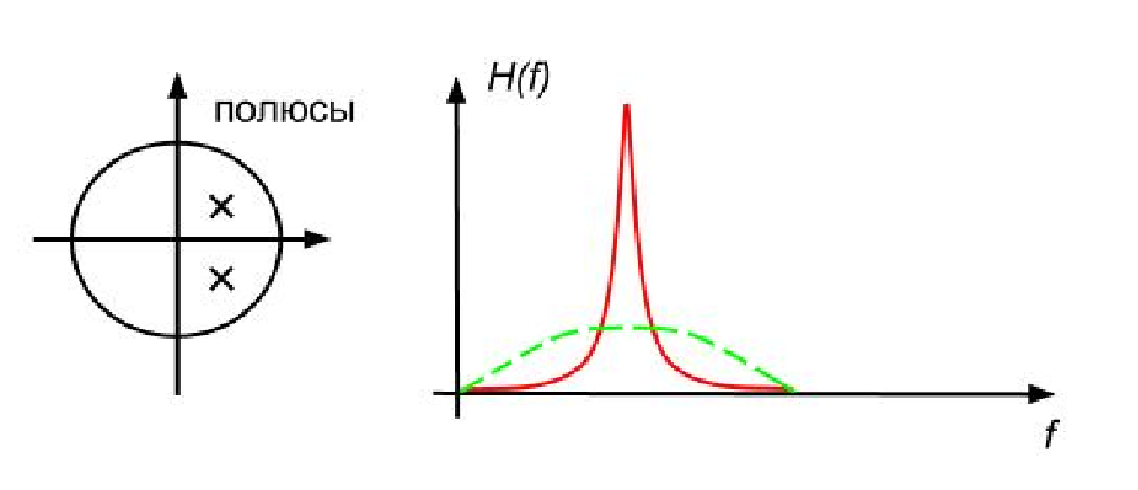
\includegraphics[width=1\linewidth]{lpc_poles_gps.eps}}
	\caption{Полюс и АЧХ линейного предсказателя}
	\label{pic:lpc_poles_gps}
\end{figure}

%%%%%%%%%%%%%%%%%%%%%%%%%%%%%%%%%%%%%%%%%%%%%%%%%%%%%%%%%%%%%%
\subsubsection{Детектирование ШПС от одного источника}
Пусть входной сигнал после снятия кода может быть представлен в виде:

\begin{center}
\begin{equation}
	\label{eq:lpc_signal_model}
	x(k)=A \cos{(\omega k)} + n(k)
\end{equation}
\end{center}

где ${n(k)}$ - АБГШ помеха. Тогда оценка АКФ сигнала ${x(k)}$:

Для уравнения \ref{eq:lpc_gps_1}, необходимо вычислить ковариации для 3 точек
${r_{xx}(0)}$, ${r_{xx}(1)}$, ${r_{xx}(2)}$, используя выражение \ref{eq:lpc_rxx_estimation}.

Можно построить график оценки СПМ для смещения,
содержащего максимальный спектральный пик - гармоническую компоненту
с наивысшей энергией - рисунок \ref{pic:lpc_psd_1} и график состоящий из максимальных спектральных пиков для каждой фазы
ПСП - рисунок \ref{pic:lpc_1sat_energy}.

\begin{figure}[H]
	\center\scalebox{0.9}{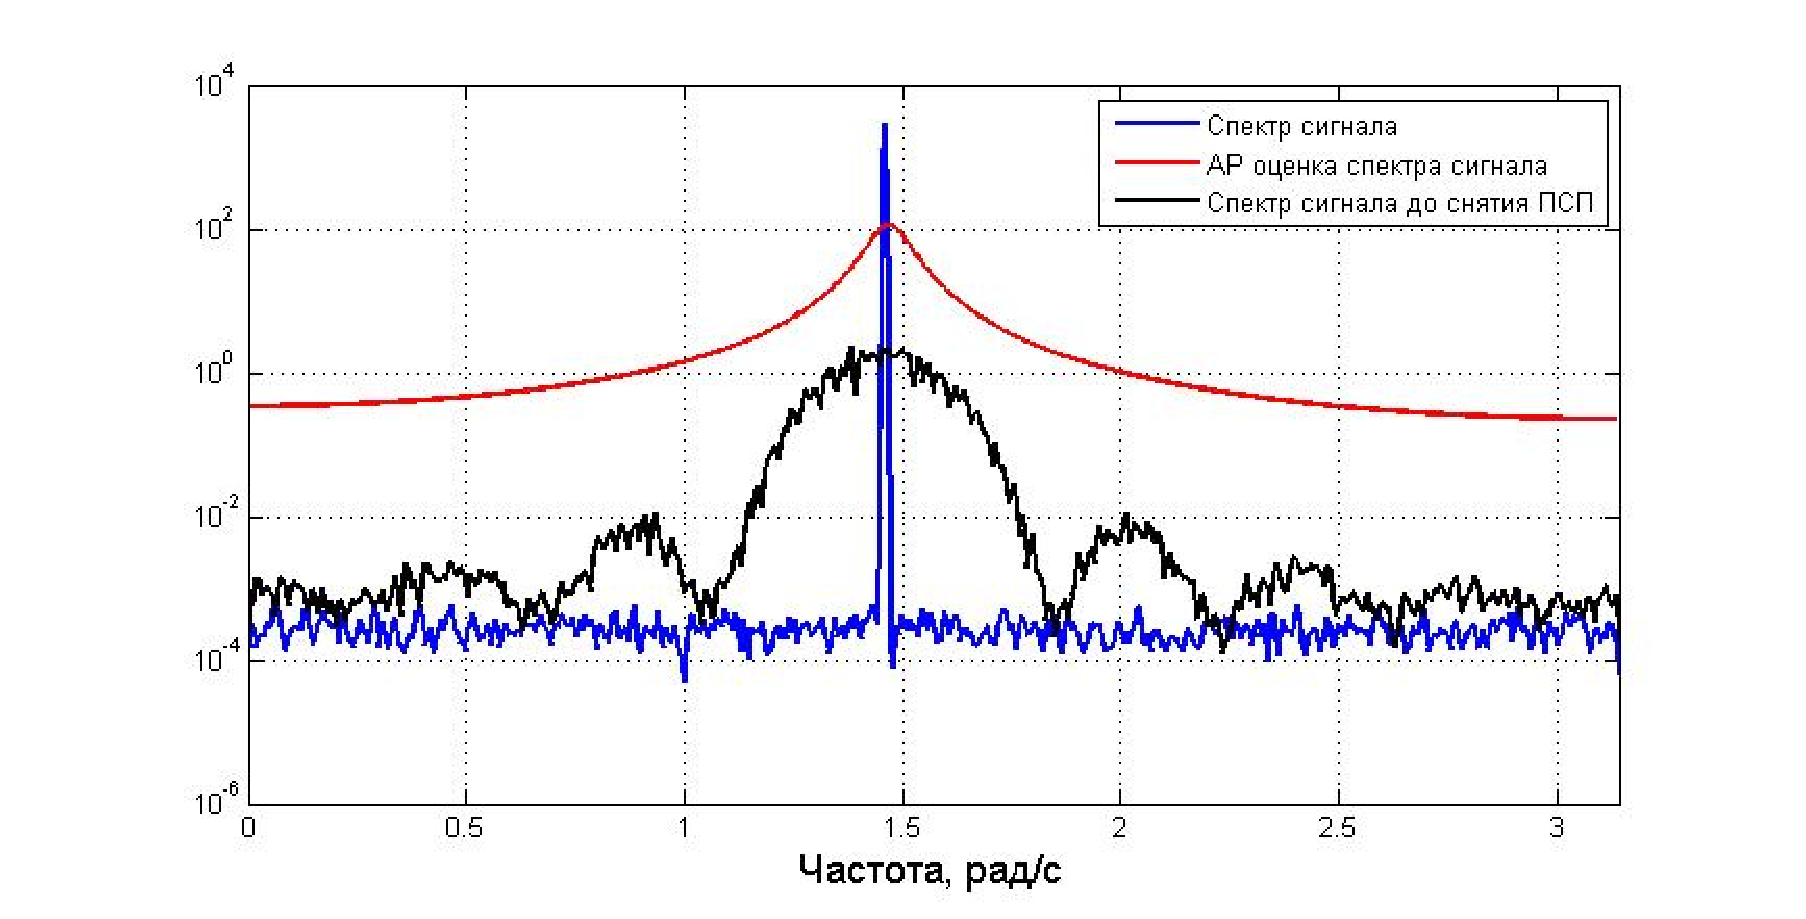
\includegraphics[width=1\linewidth]{lpc_1sat.eps}}
	\caption{Оценка СПМ сигнала модулированного ПСП}
	\label{pic:lpc_psd_1}
\end{figure}
\begin{figure}[H]
	\center\scalebox{0.9}{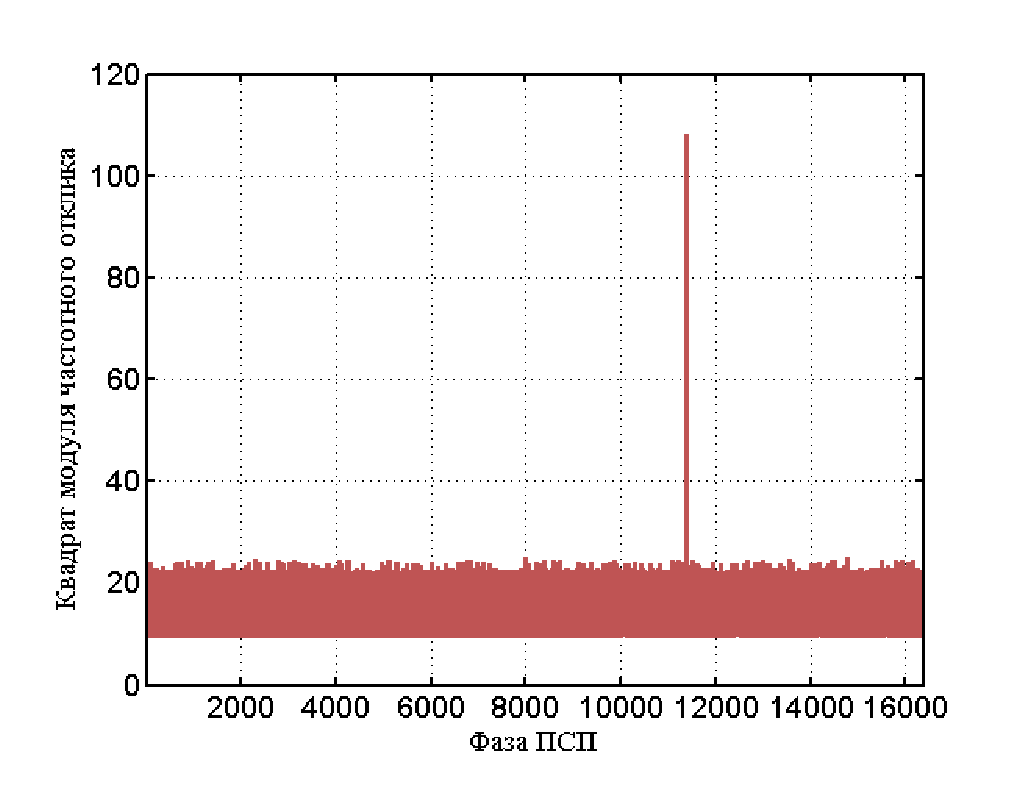
\includegraphics[width=1\linewidth]{lpc_1sat_energy.eps}}
	\caption{Максимальные пики для каждой фазы ПСП}
	\label{pic:lpc_1sat_energy}
\end{figure}

%%%%%%%%%%%%%%%%%%%%%%%%%%%%%%%%%%%%%%%%%%%%%%%%%%%%%%%%%%%%%%
\subsubsection{Влияние теплового шума на точность детектирования с помощью АР модели}

%%%%%%%%%%%%%%%%%%%%%%%%%%%%%%%%%%%%%%%%%%%%%%%%%%%%%%%%%%%%%%
\subsubsection{Влияние интерференции на точность детектирования с помощью АР модели}

Шум, отличный АБГШ будет смещать оценку частоты. На рисунке \ref{pic:lpc_2sat_psd} показано
смещение для интерференционной помехи от еще одного источника сигнала, модулированной ПСП того же семейства.
Данная помеха не является белой и оценка АР-методом по предложенному алгоритму не даст надежной оценки частоты сигнала.

\begin{figure}[H]
	\center\scalebox{0.9}{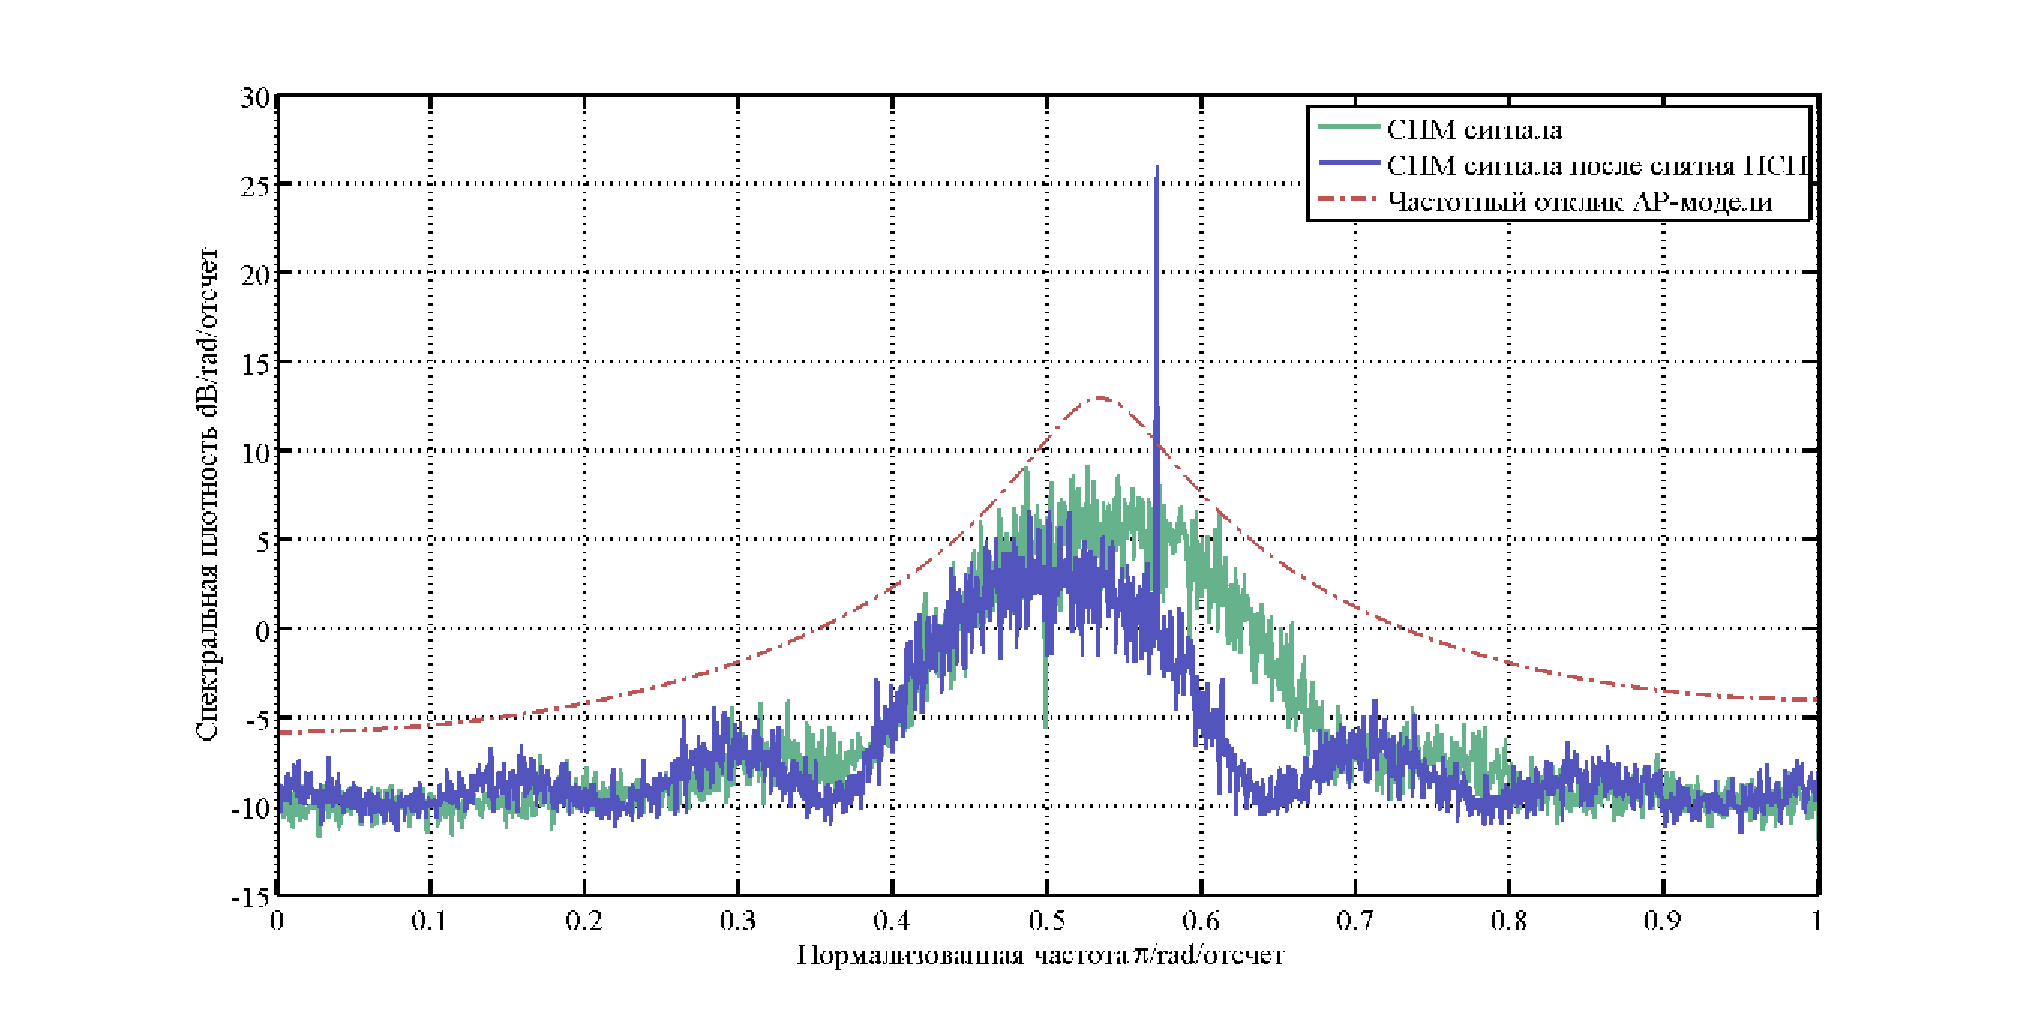
\includegraphics[width=1\linewidth]{lpc_2sat_psd.eps}}
	\caption{СПМ для сигнала с интерференционной помехой}
	\label{pic:lpc_2sat_psd}
\end{figure}

\subsection*{Выводы}

%%%%%%%%%%%%%%%%%%5
% OLD
%%%%%%%%%%%%%%%%%%5

\subsection*{\textcolor{red}{Старый текст для переноса!!!!!!!!!}}

\subsubsection{Влияние теплового шума на точность детектирования с помощью АР модели}
%Для применения АР метода является очень существенным знать модель шумовой компоненты из ${n(t)}$ из выражения
%		r_{xx}(2)
%\ref{eq:lpc_signal}. Зная АКФ ${n(t)}$, можно получить несмещенную оценки ${\omega_c}$.

\subsubsection{Детектирование ШПС от одного источника}


Но любой шум, отличный АБГШ будет смещать оценку частоты. На рисунке \ref{pic:lpc_1sat_interference}
представлен график смещения оценки в зависимости от мощности второго луча сигнала, модулированного
той же ПСП.

\begin{figure}[H]
	\center\scalebox{1}{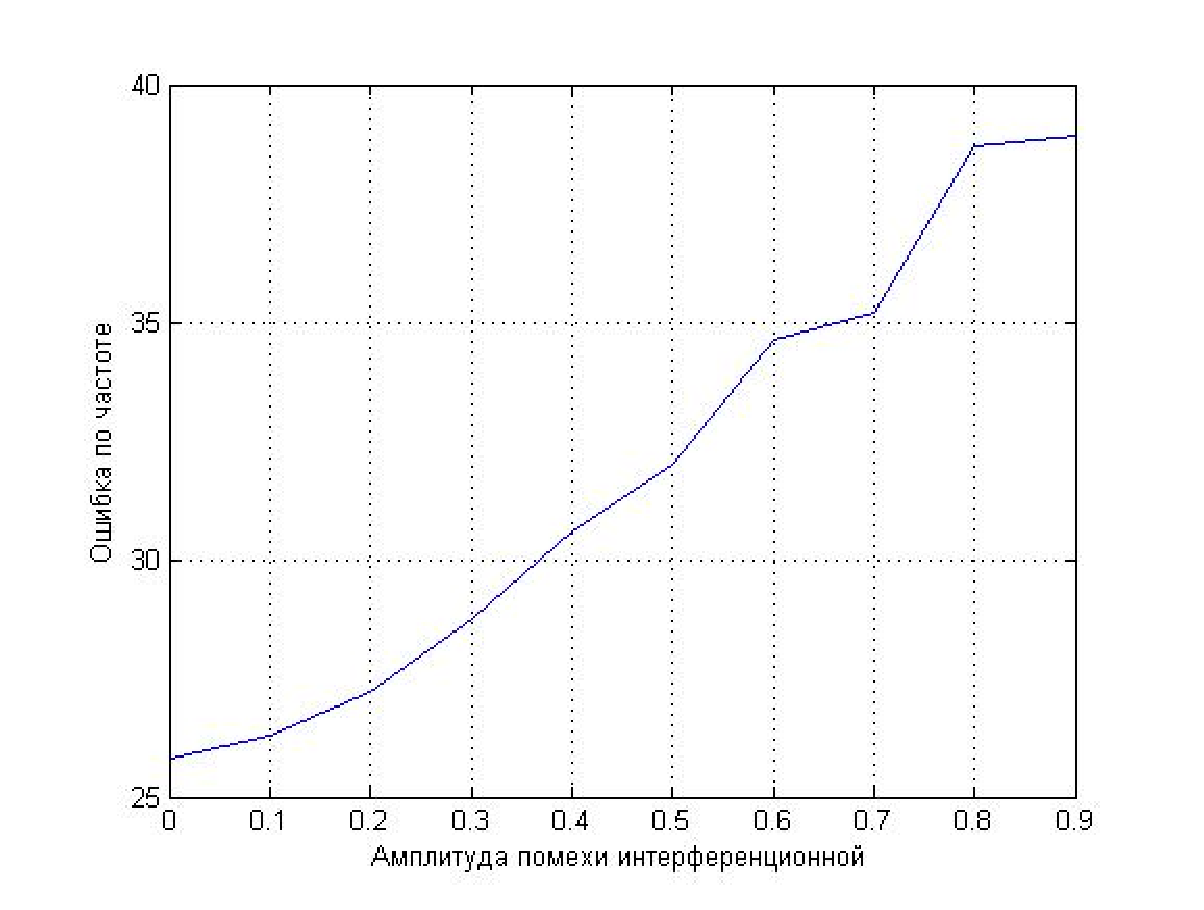
\includegraphics[width=1\linewidth]{lpc_interference.eps}}
	\caption{Зависимость ошибки оценки пика от энергии интерференционной помехи}
	\label{pic:lpc_1sat_interference}
\end{figure}

%%%%%%%%%%%%%%%%%%%%%%%%%%%%%%%%%%%%%%%%%%%%%%%
\subsubsection{Детектирование ШПС с коррекцией шума}

Для детектирования слабых сигналов, необходимо знать природу шума. Тепловой шум является одинаковым для всех источников,
таким образом его можно получить от других приемников или рассчитать в процессе детектирования. 

Для некоторых существующих систем на основе сигналов, модулированных ПСП, можно использовать приемники находящиеся рядом,
ввиду, что приемников данного сигнала достаточно большое количество. В качестве примера можно взять сигнал Navstar GPS
для приемников. Достаточно большое количество приемников GPS, захвативших сигнал, находится вблизи приемника, который
только начинает процедуру детектирования сигнала. По такой схеме работает система AGPS (Assistance GPS). Так же по данной
схеме работает система, разработанная в процессе исследований. Эта система отражена в заявке на изобретение
\cite{patent_my}.

\begin{center}
\begin{equation}
	\label{eq:lpc_a_estimation}
	\left[ \begin{array}{c}
		\hat{a}_1 \\
		\hat{a}_2
	\end{array} \right]
		=
		\left(
			\left[ \begin{array}{cc}
				r_{xx}(0) & r_{xx}(1) \\
				r_{xx}(1) & r_{xx}(0)
			\end{array} \right] -
			\left[ \begin{array}{cc}
				n_{xx}(0) & n_{xx}(1) \\
				n_{xx}(1) & n_{xx}(0)
			\end{array} \right] 
		\right)
		\left[ \begin{array}{c}
			r_{xx}(1) \\
			r_{xx}(2)
		\end{array} \right]
		=
		R_x^{-1}r_{xx1}
\end{equation}
\end{center}

%%%%%%%%%%%%%%%%%%%%%%%%%%%%%%%%%%%%%%%%%%%%%%%
\subsubsection{Детектирование ШПС с коррекцией шума}
Точность АР метода напрямую зависит от точности оценки АКФ гармонического сигнала. Основным способом повышения точности оценки
АКФ является увеличение размера выборки, что в случае модулированного сигнала может быть затруднительным. В данной работе
предлагается алгоритм оценки АКФ гармонического сигнала, не требующий увеличения длины или накопления сигнала.
Повышение точности достигается за счет того, что АКФ гармонического сигнала представляет собой гармонический сигнал той же частоты.
Пусть входной сигнал после снятия кода может быть представлен в виде:

\begin{center}
\begin{equation}
	%\label{eq:lpc_gps_1}
	x(k)=A \cos{(\omega_k)} + n(k)
\end{equation}
\end{center}

где ${n(k)}$ - АБГШ помеха. Тогда оценка АКФ сигнала ${x(k)}$:


\begin{center}
\begin{equation}
	%\label{eq:lpc_gps_1}
	r_1 = F^{-1}[Fx \cdot Fx]
\end{equation}
\end{center}

где ${F}$ - матрица преобразования Фурье, ${F^{-1}}$ - обратная матрица преобразования Фурье, ${x}$ - вектор входного сигнала,
демодулированного ПСП, а (${\cdot{}}$) - знак означает поэлементное перемножение векторов.

\begin{center}
\begin{equation}
	%\label{eq:lpc_gps_1}
	r_1 = F^{-1} \left[ F\left[F^{-1}\left[Fx \cdot Fx\right]\right] \cdot F\left[F^{-1}\left[Fx \cdot Fx\right]\right] \right]
\end{equation}
\end{center}

Специфичной для детектирования ШПС является необходимость определения точной фазы ПСП
для работы с сигналом. Так же при обработке ШПС от нескольких источников с разными ПСП необходимо учитывать,
что оценка спектра будет смещенной и требуется его корректировка. Следует учитывать, что после демодуляции
с синхронизированной копией ПСП получается гармоничнская компонента и шум. Подробнее компоненты шума были
рассмотрены в \ref{l:noise_model}. Преобразуем выражение \ref{eq:gps_signal_modulated}: амплитуду гармонического
сигнала возьмем ${\sqrt{2A} = 1}$, ${D_k(t)}$ примем за 1, учитывая, что мы детектируем сигнал в пределах одного
чипа:
\begin{center}
\begin{equation}
	\label{eq:lpc_signal}
	s(t) = \cos(\omega_{c}t) + n(t)
\end{equation}
\end{center}

Специфичной для детектирования ШПС является необходимость определения точной фазы ПСП
для работы с сигналом. Так же при обработке ШПС от нескольких источников с разными ПСП необходимо учитывать,
что оценка спектра будет смещенной и требуется его корректировка. Следует учитывать, что после демодуляции
с синхронизированной копией ПСП получается гармоничнская компонента и шум. Подробнее компоненты шума были
рассмотрены в \ref{l:noise_model}. Преобразуем выражение \ref{eq:gps_signal_modulated}: амплитуду гармонического
сигнала возьмем ${\sqrt{2A} = 1}$, ${D_k(t)}$ примем за 1, учитывая, что мы детектируем сигнал в пределах одного
чипа:
\begin{center}
\begin{equation}
	\label{eq:lpc_signal}
	s(t) = \cos(\omega_{c}t) + n(t)
\end{equation}
\end{center}

\newpage


%Литература
\clearpage
\phantomsection
\addcontentsline{toc}{chapter}{\bibname}	% Добавляем список литературы в оглавление
\bibliography{bibtex_db}
 %
\end{document}
